\begin{figure}\vspace{1cm}\hspace{0.5cm}
  % GNUPLOT: LaTeX picture with Postscript
\begingroup
  \makeatletter
  \providecommand\color[2][]{%
    \GenericError{(gnuplot) \space\space\space\@spaces}{%
      Package color not loaded in conjunction with
      terminal option `colourtext'%
    }{See the gnuplot documentation for explanation.%
    }{Either use 'blacktext' in gnuplot or load the package
      color.sty in LaTeX.}%
    \renewcommand\color[2][]{}%
  }%
  \providecommand\includegraphics[2][]{%
    \GenericError{(gnuplot) \space\space\space\@spaces}{%
      Package graphicx or graphics not loaded%
    }{See the gnuplot documentation for explanation.%
    }{The gnuplot epslatex terminal needs graphicx.sty or graphics.sty.}%
    \renewcommand\includegraphics[2][]{}%
  }%
  \providecommand\rotatebox[2]{#2}%
  \@ifundefined{ifGPcolor}{%
    \newif\ifGPcolor
    \GPcolorfalse
  }{}%
  \@ifundefined{ifGPblacktext}{%
    \newif\ifGPblacktext
    \GPblacktexttrue
  }{}%
  % define a \g@addto@macro without @ in the name:
  \let\gplgaddtomacro\g@addto@macro
  % define empty templates for all commands taking text:
  \gdef\gplbacktext{}%
  \gdef\gplfronttext{}%
  \makeatother
  \ifGPblacktext
    % no textcolor at all
    \def\colorrgb#1{}%
    \def\colorgray#1{}%
  \else
    % gray or color?
    \ifGPcolor
      \def\colorrgb#1{\color[rgb]{#1}}%
      \def\colorgray#1{\color[gray]{#1}}%
      \expandafter\def\csname LTw\endcsname{\color{white}}%
      \expandafter\def\csname LTb\endcsname{\color{black}}%
      \expandafter\def\csname LTa\endcsname{\color{black}}%
      \expandafter\def\csname LT0\endcsname{\color[rgb]{1,0,0}}%
      \expandafter\def\csname LT1\endcsname{\color[rgb]{0,1,0}}%
      \expandafter\def\csname LT2\endcsname{\color[rgb]{0,0,1}}%
      \expandafter\def\csname LT3\endcsname{\color[rgb]{1,0,1}}%
      \expandafter\def\csname LT4\endcsname{\color[rgb]{0,1,1}}%
      \expandafter\def\csname LT5\endcsname{\color[rgb]{1,1,0}}%
      \expandafter\def\csname LT6\endcsname{\color[rgb]{0,0,0}}%
      \expandafter\def\csname LT7\endcsname{\color[rgb]{1,0.3,0}}%
      \expandafter\def\csname LT8\endcsname{\color[rgb]{0.5,0.5,0.5}}%
    \else
      % gray
      \def\colorrgb#1{\color{black}}%
      \def\colorgray#1{\color[gray]{#1}}%
      \expandafter\def\csname LTw\endcsname{\color{white}}%
      \expandafter\def\csname LTb\endcsname{\color{black}}%
      \expandafter\def\csname LTa\endcsname{\color{black}}%
      \expandafter\def\csname LT0\endcsname{\color{black}}%
      \expandafter\def\csname LT1\endcsname{\color{black}}%
      \expandafter\def\csname LT2\endcsname{\color{black}}%
      \expandafter\def\csname LT3\endcsname{\color{black}}%
      \expandafter\def\csname LT4\endcsname{\color{black}}%
      \expandafter\def\csname LT5\endcsname{\color{black}}%
      \expandafter\def\csname LT6\endcsname{\color{black}}%
      \expandafter\def\csname LT7\endcsname{\color{black}}%
      \expandafter\def\csname LT8\endcsname{\color{black}}%
    \fi
  \fi
  \setlength{\unitlength}{0.0500bp}%
  \begin{picture}(8000.00,8000.00)%
     \gplgaddtomacro\gplfronttext{%
      \colorrgb{0.00,0.00,0.00}%
      \put(716,8200){\makebox(0,0){\strut{}\small $\sigma_R = 0.01$}}%
      \colorrgb{0.00,0.00,0.00}%
      \put(2029,8200){\makebox(0,0){\strut{}\small $\sigma_R = 0.03$}}%
      \colorrgb{0.00,0.00,0.00}%
      \put(3343,8200){\makebox(0,0){\strut{}\small $\sigma_R = 0.05$}}%
      \colorrgb{0.00,0.00,0.00}%
      \put(4656,8200){\makebox(0,0){\strut{}\small $\sigma_R = 0.10$}}%
      \colorrgb{0.00,0.00,0.00}%
      \put(5969,8200){\makebox(0,0){\strut{}\small $\sigma_R = 0.20$ [m]}}%
    }%
    \gplgaddtomacro\gplfronttext{%
      \colorrgb{0.00,0.00,0.00}%
      \put(-200,7333.33){\rotatebox{90}{\makebox(0,0){\strut{}\small PLICP}}}%
    }%
    \gplgaddtomacro\gplfronttext{%
      \colorrgb{0.00,0.00,0.00}%
      \put(-200,6000){\rotatebox{90}{\makebox(0,0){\strut{}\small NDT}}}%
    }%
    \gplgaddtomacro\gplfronttext{%
      \colorrgb{0.00,0.00,0.00}%
      \put(-200,4666.66){\rotatebox{90}{\makebox(0,0){\strut{}\small FastGICP}}}%
    }%
    \gplgaddtomacro\gplfronttext{%
      \colorrgb{0.00,0.00,0.00}%
      \put(-200,3333.33){\rotatebox{90}{\makebox(0,0){\strut{}\small FastVGICP}}}%
    }%
    \gplgaddtomacro\gplfronttext{%
      \colorrgb{0.00,0.00,0.00}%
      \put(-200,2000){\rotatebox{90}{\makebox(0,0){\strut{}\small NDT-PSO}}}%
    }%
    \gplgaddtomacro\gplfronttext{%
      \colorrgb{0.00,0.00,0.00}%
      \put(-200,666.66){\rotatebox{90}{\makebox(0,0){\strut{}\small \texttt{fsm}}}}%
    }%
    \gplgaddtomacro\gplfronttext{%
      \colorrgb{0.00,0.00,0.00}%
      \put(7800,515.5){\makebox(0,0)[l]{\strut{}$<0.001$}}%
      \colorrgb{0.00,0.00,0.00}%
      \put(7800,1386.5){\makebox(0,0)[l]{\strut{}$<0.01$}}%
      \colorrgb{0.00,0.0.00,0.00}%
      \put(7800,2257.5){\makebox(0,0)[l]{\strut{}$<0.05$}}%
      \colorrgb{0.00,0.0.00,0.00}%
      \put(7800,3128.5){\makebox(0,0)[l]{\strut{}$<0.1$}}%
      \colorrgb{0.00,0.0.00,0.00}%
      \put(7800,3999.5){\makebox(0,0)[l]{\strut{}$<0.15$}}%
      \colorrgb{0.00,0.0.00,0.00}%
      \put(7800,4870.5){\makebox(0,0)[l]{\strut{}$<0.2$}}%
      \colorrgb{0.00,0.0.00,0.00}%
      \put(7800,5741.5){\makebox(0,0)[l]{\strut{}$<0.25$}}%
      \colorrgb{0.00,0.0.00,0.00}%
      \put(7800,6612.5){\makebox(0,0)[l]{\strut{}$<0.5$}}%
      \colorrgb{0.00,0.00,0.00}%
      \put(7800,7483.5){\makebox(0,0)[l]{\strut{}$<77.609$}}%
    }%
    \put(0,0){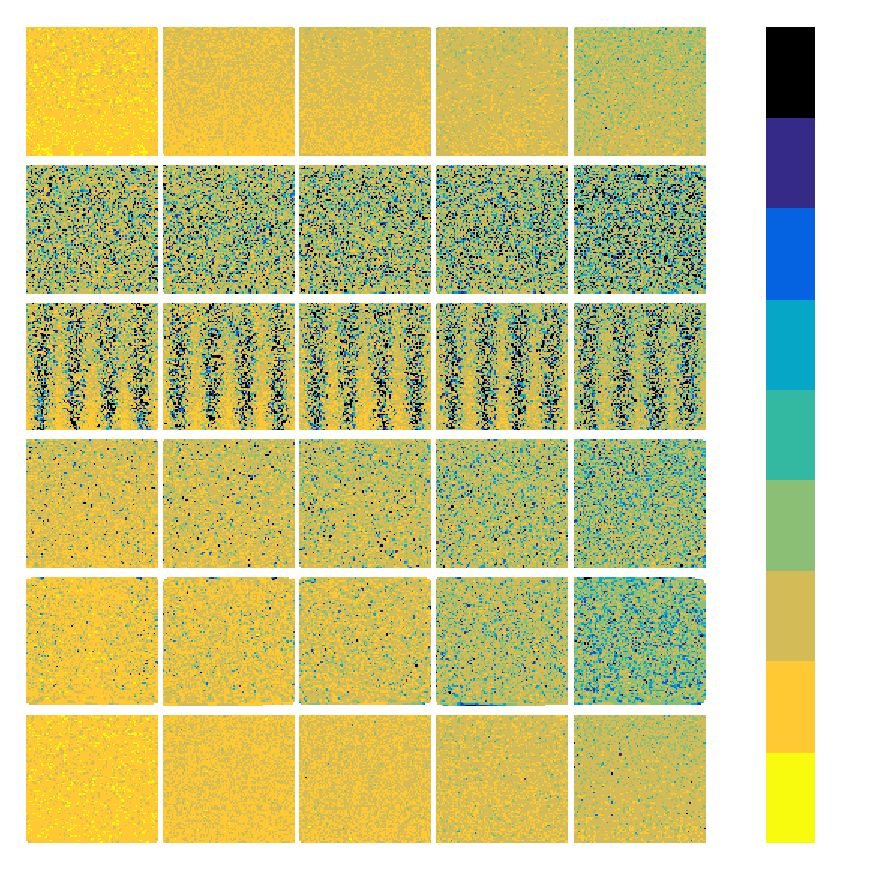
\includegraphics{./figures/parts/appendix/chapters/05/sections/04/caer_style_position_errors_binned_dxyt1}}%
    \gplfronttext
  \end{picture}%
\endgroup

  \vspace{1cm}
  \caption{\small Χάρτες θερμότητας των μέτρων των τελικών σφαλμάτων εκτίμησης
           θέσης συναρτήσει των αρχικών σφαλμάτων εκτίμησης προσανατολισμού
           $\Delta\hat{\theta} \in
           [-\overline{\delta}_{\theta},+\overline{\delta}_{\theta}]$ (στον
           οριζόντιο άξονα) και των μέτρων των αρχικών σφαλμάτων εκτίμησης
           θέσης $\|\Delta \hat{\bm{l}}\|_2 \in [0, \sqrt{2}\cdot
           \overline{\delta}_{xy}]$ (στον κάθετο άξονα) για όλα τα
           διενεργηθέντα πειράματα, ανά αλγόριθμο και ανά τυπική απόκλιση
           διαταραχών του φυσικού αισθητήρα, για τη διάταξη με
           $(\overline{\delta}_{xy}, \overline{\delta}_{\theta}) = (0.05,
           0.035)$ [m,rad]}
  \label{fig:appendix_05_01:01}
\end{figure}
\begin{figure}\vspace{1cm}\hspace{0.5cm}
  % GNUPLOT: LaTeX picture with Postscript
\begingroup
  \makeatletter
  \providecommand\color[2][]{%
    \GenericError{(gnuplot) \space\space\space\@spaces}{%
      Package color not loaded in conjunction with
      terminal option `colourtext'%
    }{See the gnuplot documentation for explanation.%
    }{Either use 'blacktext' in gnuplot or load the package
      color.sty in LaTeX.}%
    \renewcommand\color[2][]{}%
  }%
  \providecommand\includegraphics[2][]{%
    \GenericError{(gnuplot) \space\space\space\@spaces}{%
      Package graphicx or graphics not loaded%
    }{See the gnuplot documentation for explanation.%
    }{The gnuplot epslatex terminal needs graphicx.sty or graphics.sty.}%
    \renewcommand\includegraphics[2][]{}%
  }%
  \providecommand\rotatebox[2]{#2}%
  \@ifundefined{ifGPcolor}{%
    \newif\ifGPcolor
    \GPcolorfalse
  }{}%
  \@ifundefined{ifGPblacktext}{%
    \newif\ifGPblacktext
    \GPblacktexttrue
  }{}%
  % define a \g@addto@macro without @ in the name:
  \let\gplgaddtomacro\g@addto@macro
  % define empty templates for all commands taking text:
  \gdef\gplbacktext{}%
  \gdef\gplfronttext{}%
  \makeatother
  \ifGPblacktext
    % no textcolor at all
    \def\colorrgb#1{}%
    \def\colorgray#1{}%
  \else
    % gray or color?
    \ifGPcolor
      \def\colorrgb#1{\color[rgb]{#1}}%
      \def\colorgray#1{\color[gray]{#1}}%
      \expandafter\def\csname LTw\endcsname{\color{white}}%
      \expandafter\def\csname LTb\endcsname{\color{black}}%
      \expandafter\def\csname LTa\endcsname{\color{black}}%
      \expandafter\def\csname LT0\endcsname{\color[rgb]{1,0,0}}%
      \expandafter\def\csname LT1\endcsname{\color[rgb]{0,1,0}}%
      \expandafter\def\csname LT2\endcsname{\color[rgb]{0,0,1}}%
      \expandafter\def\csname LT3\endcsname{\color[rgb]{1,0,1}}%
      \expandafter\def\csname LT4\endcsname{\color[rgb]{0,1,1}}%
      \expandafter\def\csname LT5\endcsname{\color[rgb]{1,1,0}}%
      \expandafter\def\csname LT6\endcsname{\color[rgb]{0,0,0}}%
      \expandafter\def\csname LT7\endcsname{\color[rgb]{1,0.3,0}}%
      \expandafter\def\csname LT8\endcsname{\color[rgb]{0.5,0.5,0.5}}%
    \else
      % gray
      \def\colorrgb#1{\color{black}}%
      \def\colorgray#1{\color[gray]{#1}}%
      \expandafter\def\csname LTw\endcsname{\color{white}}%
      \expandafter\def\csname LTb\endcsname{\color{black}}%
      \expandafter\def\csname LTa\endcsname{\color{black}}%
      \expandafter\def\csname LT0\endcsname{\color{black}}%
      \expandafter\def\csname LT1\endcsname{\color{black}}%
      \expandafter\def\csname LT2\endcsname{\color{black}}%
      \expandafter\def\csname LT3\endcsname{\color{black}}%
      \expandafter\def\csname LT4\endcsname{\color{black}}%
      \expandafter\def\csname LT5\endcsname{\color{black}}%
      \expandafter\def\csname LT6\endcsname{\color{black}}%
      \expandafter\def\csname LT7\endcsname{\color{black}}%
      \expandafter\def\csname LT8\endcsname{\color{black}}%
    \fi
  \fi
  \setlength{\unitlength}{0.0500bp}%
  \begin{picture}(8000.00,8000.00)%
     \gplgaddtomacro\gplfronttext{%
      \colorrgb{0.00,0.00,0.00}%
      \put(716,8200){\makebox(0,0){\strut{}\small $\sigma_R = 0.01$}}%
      \colorrgb{0.00,0.00,0.00}%
      \put(2029,8200){\makebox(0,0){\strut{}\small $\sigma_R = 0.03$}}%
      \colorrgb{0.00,0.00,0.00}%
      \put(3343,8200){\makebox(0,0){\strut{}\small $\sigma_R = 0.05$}}%
      \colorrgb{0.00,0.00,0.00}%
      \put(4656,8200){\makebox(0,0){\strut{}\small $\sigma_R = 0.10$}}%
      \colorrgb{0.00,0.00,0.00}%
      \put(5969,8200){\makebox(0,0){\strut{}\small $\sigma_R = 0.20$ [m]}}%
      \put(3333.33,8700){\makebox(0,0){\strut{}$(\overline{\delta}_{xy}, \overline{\delta}_\theta) = (0.10 \ \text{m}, 0.07 \ \text{rad})$}}
      \put(4000,9200){\makebox(0,0){\strut{}Τελικά σφάλματα εκτίμησης θέσης ως προς αρχικές συνθήκες μετατόπισης [m]}}
    }%
    \gplgaddtomacro\gplfronttext{%
      \colorrgb{0.00,0.00,0.00}%
      \put(-200,7333.33){\rotatebox{90}{\makebox(0,0){\strut{}\small PLICP}}}%
    }%
    \gplgaddtomacro\gplfronttext{%
      \colorrgb{0.00,0.00,0.00}%
      \put(-200,6000){\rotatebox{90}{\makebox(0,0){\strut{}\small NDT}}}%
    }%
    \gplgaddtomacro\gplfronttext{%
      \colorrgb{0.00,0.00,0.00}%
      \put(-200,4666.66){\rotatebox{90}{\makebox(0,0){\strut{}\small FastGICP}}}%
    }%
    \gplgaddtomacro\gplfronttext{%
      \colorrgb{0.00,0.00,0.00}%
      \put(-200,3333.33){\rotatebox{90}{\makebox(0,0){\strut{}\small FastVGICP}}}%
    }%
    \gplgaddtomacro\gplfronttext{%
      \colorrgb{0.00,0.00,0.00}%
      \put(-200,2000){\rotatebox{90}{\makebox(0,0){\strut{}\small NDT-PSO}}}%
    }%
    \gplgaddtomacro\gplfronttext{%
      \colorrgb{0.00,0.00,0.00}%
      \put(-200,666.66){\rotatebox{90}{\makebox(0,0){\strut{}\small \texttt{fsm}}}}%
    }%
    \gplgaddtomacro\gplfronttext{%
      \colorrgb{0.00,0.00,0.00}%
      \colorrgb{0.00,0.00,0.00}%
      \put(7800,515.5){\makebox(0,0)[l]{\strut{}$<0.001$}}%
      \colorrgb{0.00,0.00,0.00}%
      \put(7800,1386.5){\makebox(0,0)[l]{\strut{}$<0.01$}}%
      \colorrgb{0.00,0.0.00,0.00}%
      \put(7800,2257.5){\makebox(0,0)[l]{\strut{}$<0.05$}}%
      \colorrgb{0.00,0.0.00,0.00}%
      \put(7800,3128.5){\makebox(0,0)[l]{\strut{}$<0.1$}}%
      \colorrgb{0.00,0.0.00,0.00}%
      \put(7800,3999.5){\makebox(0,0)[l]{\strut{}$<0.15$}}%
      \colorrgb{0.00,0.0.00,0.00}%
      \put(7800,4870.5){\makebox(0,0)[l]{\strut{}$<0.2$}}%
      \colorrgb{0.00,0.0.00,0.00}%
      \put(7800,5741.5){\makebox(0,0)[l]{\strut{}$<0.25$}}%
      \colorrgb{0.00,0.0.00,0.00}%
      \put(7800,6612.5){\makebox(0,0)[l]{\strut{}$<0.5$}}%
      \colorrgb{0.00,0.00,0.00}%
      \put(7800,7483.5){\makebox(0,0)[l]{\strut{}$<e^{\overline{\delta}_{xy}, \overline{\delta}_\theta}_{xy,\max} = 64.4$}}%
    }%
    \put(0,0){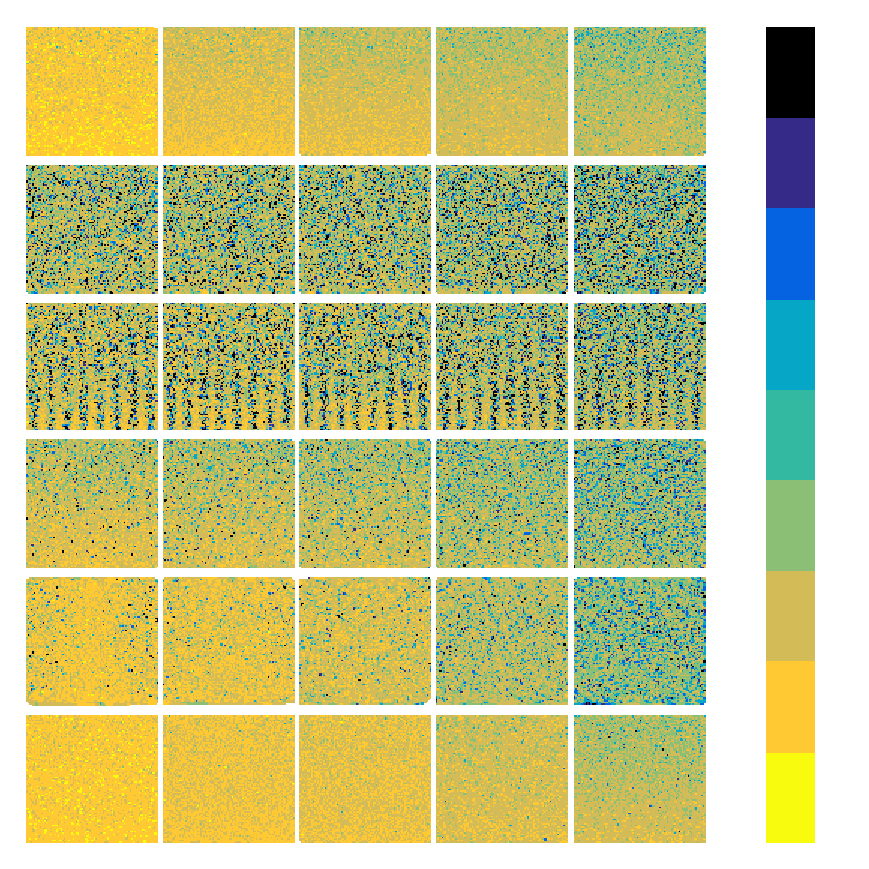
\includegraphics{./figures/parts/appendix/chapters/05/sections/04/caer_style_position_errors_binned_dxyt2}}%
    \gplfronttext
  \end{picture}%
\endgroup

  \vspace{1cm}
  \caption{\small Χάρτες θερμότητας των μέτρων των τελικών σφαλμάτων εκτίμησης
           θέσης συναρτήσει των αρχικών σφαλμάτων εκτίμησης προσανατολισμού
           $\Delta\hat{\theta} \in
           [-\overline{\delta}_{\theta},+\overline{\delta}_{\theta}]$ (στον
           οριζόντιο άξονα) και των μέτρων των αρχικών σφαλμάτων εκτίμησης
           θέσης $\|\Delta \hat{\bm{l}}\|_2 \in [0, \sqrt{2}\cdot
           \overline{\delta}_{xy}]$ (στον κάθετο άξονα) για όλα τα
           διενεργηθέντα πειράματα, ανά αλγόριθμο και ανά τυπική απόκλιση
           διαταραχών του φυσικού αισθητήρα, για τη διάταξη με
           $(\overline{\delta}_{xy}, \overline{\delta}_{\theta}) = (0.10,
           0.070)$ [m,rad]}
  \label{fig:appendix_05_01:02}
\end{figure}
\begin{figure}\vspace{1cm}\hspace{0.5cm}
  % GNUPLOT: LaTeX picture with Postscript
\begingroup
  \makeatletter
  \providecommand\color[2][]{%
    \GenericError{(gnuplot) \space\space\space\@spaces}{%
      Package color not loaded in conjunction with
      terminal option `colourtext'%
    }{See the gnuplot documentation for explanation.%
    }{Either use 'blacktext' in gnuplot or load the package
      color.sty in LaTeX.}%
    \renewcommand\color[2][]{}%
  }%
  \providecommand\includegraphics[2][]{%
    \GenericError{(gnuplot) \space\space\space\@spaces}{%
      Package graphicx or graphics not loaded%
    }{See the gnuplot documentation for explanation.%
    }{The gnuplot epslatex terminal needs graphicx.sty or graphics.sty.}%
    \renewcommand\includegraphics[2][]{}%
  }%
  \providecommand\rotatebox[2]{#2}%
  \@ifundefined{ifGPcolor}{%
    \newif\ifGPcolor
    \GPcolorfalse
  }{}%
  \@ifundefined{ifGPblacktext}{%
    \newif\ifGPblacktext
    \GPblacktexttrue
  }{}%
  % define a \g@addto@macro without @ in the name:
  \let\gplgaddtomacro\g@addto@macro
  % define empty templates for all commands taking text:
  \gdef\gplbacktext{}%
  \gdef\gplfronttext{}%
  \makeatother
  \ifGPblacktext
    % no textcolor at all
    \def\colorrgb#1{}%
    \def\colorgray#1{}%
  \else
    % gray or color?
    \ifGPcolor
      \def\colorrgb#1{\color[rgb]{#1}}%
      \def\colorgray#1{\color[gray]{#1}}%
      \expandafter\def\csname LTw\endcsname{\color{white}}%
      \expandafter\def\csname LTb\endcsname{\color{black}}%
      \expandafter\def\csname LTa\endcsname{\color{black}}%
      \expandafter\def\csname LT0\endcsname{\color[rgb]{1,0,0}}%
      \expandafter\def\csname LT1\endcsname{\color[rgb]{0,1,0}}%
      \expandafter\def\csname LT2\endcsname{\color[rgb]{0,0,1}}%
      \expandafter\def\csname LT3\endcsname{\color[rgb]{1,0,1}}%
      \expandafter\def\csname LT4\endcsname{\color[rgb]{0,1,1}}%
      \expandafter\def\csname LT5\endcsname{\color[rgb]{1,1,0}}%
      \expandafter\def\csname LT6\endcsname{\color[rgb]{0,0,0}}%
      \expandafter\def\csname LT7\endcsname{\color[rgb]{1,0.3,0}}%
      \expandafter\def\csname LT8\endcsname{\color[rgb]{0.5,0.5,0.5}}%
    \else
      % gray
      \def\colorrgb#1{\color{black}}%
      \def\colorgray#1{\color[gray]{#1}}%
      \expandafter\def\csname LTw\endcsname{\color{white}}%
      \expandafter\def\csname LTb\endcsname{\color{black}}%
      \expandafter\def\csname LTa\endcsname{\color{black}}%
      \expandafter\def\csname LT0\endcsname{\color{black}}%
      \expandafter\def\csname LT1\endcsname{\color{black}}%
      \expandafter\def\csname LT2\endcsname{\color{black}}%
      \expandafter\def\csname LT3\endcsname{\color{black}}%
      \expandafter\def\csname LT4\endcsname{\color{black}}%
      \expandafter\def\csname LT5\endcsname{\color{black}}%
      \expandafter\def\csname LT6\endcsname{\color{black}}%
      \expandafter\def\csname LT7\endcsname{\color{black}}%
      \expandafter\def\csname LT8\endcsname{\color{black}}%
    \fi
  \fi
  \setlength{\unitlength}{0.0500bp}%
  \begin{picture}(8000.00,8000.00)%
     \gplgaddtomacro\gplfronttext{%
      \colorrgb{0.00,0.00,0.00}%
      \put(716,8200){\makebox(0,0){\strut{}\small $\sigma_R = 0.01$}}%
      \colorrgb{0.00,0.00,0.00}%
      \put(2029,8200){\makebox(0,0){\strut{}\small $\sigma_R = 0.03$}}%
      \colorrgb{0.00,0.00,0.00}%
      \put(3343,8200){\makebox(0,0){\strut{}\small $\sigma_R = 0.05$}}%
      \colorrgb{0.00,0.00,0.00}%
      \put(4656,8200){\makebox(0,0){\strut{}\small $\sigma_R = 0.10$}}%
      \colorrgb{0.00,0.00,0.00}%
      \put(5969,8200){\makebox(0,0){\strut{}\small $\sigma_R = 0.20$ [m]}}%
      \put(3333.33,8700){\makebox(0,0){\strut{}$(\overline{\delta}_{xy}, \overline{\delta}_\theta) = (0.15 \ \text{m}, 0.15 \ \text{rad})$}}
      \put(4000,9200){\makebox(0,0){\strut{}Τελικά σφάλματα εκτίμησης θέσης ως προς αρχικές συνθήκες μετατόπισης [m]}}
    }%
    \gplgaddtomacro\gplfronttext{%
      \colorrgb{0.00,0.00,0.00}%
      \put(-200,7333.33){\rotatebox{90}{\makebox(0,0){\strut{}\small PLICP}}}%
    }%
    \gplgaddtomacro\gplfronttext{%
      \colorrgb{0.00,0.00,0.00}%
      \put(-200,6000){\rotatebox{90}{\makebox(0,0){\strut{}\small NDT}}}%
    }%
    \gplgaddtomacro\gplfronttext{%
      \colorrgb{0.00,0.00,0.00}%
      \put(-200,4666.66){\rotatebox{90}{\makebox(0,0){\strut{}\small FastGICP}}}%
    }%
    \gplgaddtomacro\gplfronttext{%
      \colorrgb{0.00,0.00,0.00}%
      \put(-200,3333.33){\rotatebox{90}{\makebox(0,0){\strut{}\small FastVGICP}}}%
    }%
    \gplgaddtomacro\gplfronttext{%
      \colorrgb{0.00,0.00,0.00}%
      \put(-200,2000){\rotatebox{90}{\makebox(0,0){\strut{}\small NDT-PSO}}}%
    }%
    \gplgaddtomacro\gplfronttext{%
      \colorrgb{0.00,0.00,0.00}%
      \put(-200,666.66){\rotatebox{90}{\makebox(0,0){\strut{}\small \texttt{fsm}}}}%
    }%
    \gplgaddtomacro\gplfronttext{%
      \colorrgb{0.00,0.00,0.00}%
      \put(7800,515.5){\makebox(0,0)[l]{\strut{}$<0.001$}}%
      \colorrgb{0.00,0.00,0.00}%
      \put(7800,1386.5){\makebox(0,0)[l]{\strut{}$<0.01$}}%
      \colorrgb{0.00,0.0.00,0.00}%
      \put(7800,2257.5){\makebox(0,0)[l]{\strut{}$<0.05$}}%
      \colorrgb{0.00,0.0.00,0.00}%
      \put(7800,3128.5){\makebox(0,0)[l]{\strut{}$<0.1$}}%
      \colorrgb{0.00,0.0.00,0.00}%
      \put(7800,3999.5){\makebox(0,0)[l]{\strut{}$<0.15$}}%
      \colorrgb{0.00,0.0.00,0.00}%
      \put(7800,4870.5){\makebox(0,0)[l]{\strut{}$<0.2$}}%
      \colorrgb{0.00,0.0.00,0.00}%
      \put(7800,5741.5){\makebox(0,0)[l]{\strut{}$<0.25$}}%
      \colorrgb{0.00,0.0.00,0.00}%
      \put(7800,6612.5){\makebox(0,0)[l]{\strut{}$<0.5$}}%
      \colorrgb{0.00,0.00,0.00}%
      \put(7800,7483.5){\makebox(0,0)[l]{\strut{}$<e^{\overline{\delta}_{xy}, \overline{\delta}_\theta}_{xy,\max} = 199.6$}}%
    }%
    \put(0,0){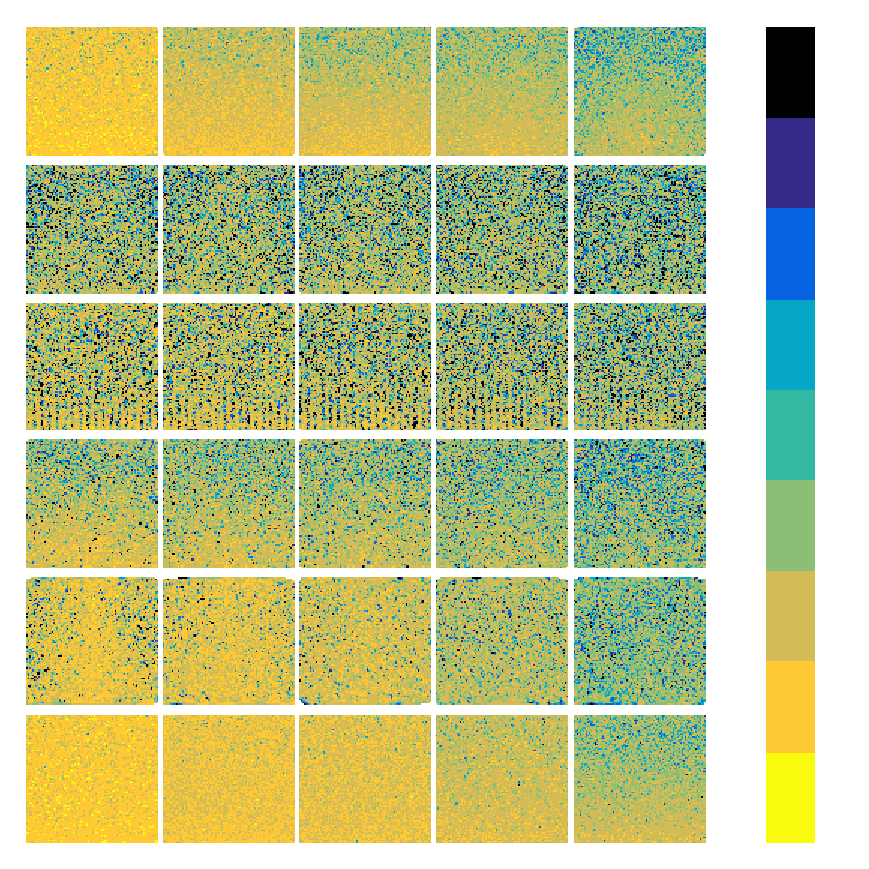
\includegraphics{./figures/parts/appendix/chapters/05/sections/04/caer_style_position_errors_binned_dxyt3}}%
    \gplfronttext
  \end{picture}%
\endgroup

  \vspace{1cm}
  \caption{\small Χάρτες θερμότητας των μέτρων των τελικών σφαλμάτων εκτίμησης
           θέσης συναρτήσει των αρχικών σφαλμάτων εκτίμησης προσανατολισμού
           $\Delta\hat{\theta} \in
           [-\overline{\delta}_{\theta},+\overline{\delta}_{\theta}]$ (στον
           οριζόντιο άξονα) και των μέτρων των αρχικών σφαλμάτων εκτίμησης
           θέσης $\|\Delta \hat{\bm{l}}\|_2 \in [0, \sqrt{2}\cdot
           \overline{\delta}_{xy}]$ (στον κάθετο άξονα) για όλα τα
           διενεργηθέντα πειράματα, ανά αλγόριθμο και ανά τυπική απόκλιση
           διαταραχών του φυσικού αισθητήρα, για τη διάταξη με
           $(\overline{\delta}_{xy}, \overline{\delta}_{\theta}) = (0.15,
           0.150)$ [m,rad]}
  \label{fig:appendix_05_01:03}
\end{figure}
\begin{figure}\vspace{1cm}\hspace{0.5cm}
  % GNUPLOT: LaTeX picture with Postscript
\begingroup
  \makeatletter
  \providecommand\color[2][]{%
    \GenericError{(gnuplot) \space\space\space\@spaces}{%
      Package color not loaded in conjunction with
      terminal option `colourtext'%
    }{See the gnuplot documentation for explanation.%
    }{Either use 'blacktext' in gnuplot or load the package
      color.sty in LaTeX.}%
    \renewcommand\color[2][]{}%
  }%
  \providecommand\includegraphics[2][]{%
    \GenericError{(gnuplot) \space\space\space\@spaces}{%
      Package graphicx or graphics not loaded%
    }{See the gnuplot documentation for explanation.%
    }{The gnuplot epslatex terminal needs graphicx.sty or graphics.sty.}%
    \renewcommand\includegraphics[2][]{}%
  }%
  \providecommand\rotatebox[2]{#2}%
  \@ifundefined{ifGPcolor}{%
    \newif\ifGPcolor
    \GPcolorfalse
  }{}%
  \@ifundefined{ifGPblacktext}{%
    \newif\ifGPblacktext
    \GPblacktexttrue
  }{}%
  % define a \g@addto@macro without @ in the name:
  \let\gplgaddtomacro\g@addto@macro
  % define empty templates for all commands taking text:
  \gdef\gplbacktext{}%
  \gdef\gplfronttext{}%
  \makeatother
  \ifGPblacktext
    % no textcolor at all
    \def\colorrgb#1{}%
    \def\colorgray#1{}%
  \else
    % gray or color?
    \ifGPcolor
      \def\colorrgb#1{\color[rgb]{#1}}%
      \def\colorgray#1{\color[gray]{#1}}%
      \expandafter\def\csname LTw\endcsname{\color{white}}%
      \expandafter\def\csname LTb\endcsname{\color{black}}%
      \expandafter\def\csname LTa\endcsname{\color{black}}%
      \expandafter\def\csname LT0\endcsname{\color[rgb]{1,0,0}}%
      \expandafter\def\csname LT1\endcsname{\color[rgb]{0,1,0}}%
      \expandafter\def\csname LT2\endcsname{\color[rgb]{0,0,1}}%
      \expandafter\def\csname LT3\endcsname{\color[rgb]{1,0,1}}%
      \expandafter\def\csname LT4\endcsname{\color[rgb]{0,1,1}}%
      \expandafter\def\csname LT5\endcsname{\color[rgb]{1,1,0}}%
      \expandafter\def\csname LT6\endcsname{\color[rgb]{0,0,0}}%
      \expandafter\def\csname LT7\endcsname{\color[rgb]{1,0.3,0}}%
      \expandafter\def\csname LT8\endcsname{\color[rgb]{0.5,0.5,0.5}}%
    \else
      % gray
      \def\colorrgb#1{\color{black}}%
      \def\colorgray#1{\color[gray]{#1}}%
      \expandafter\def\csname LTw\endcsname{\color{white}}%
      \expandafter\def\csname LTb\endcsname{\color{black}}%
      \expandafter\def\csname LTa\endcsname{\color{black}}%
      \expandafter\def\csname LT0\endcsname{\color{black}}%
      \expandafter\def\csname LT1\endcsname{\color{black}}%
      \expandafter\def\csname LT2\endcsname{\color{black}}%
      \expandafter\def\csname LT3\endcsname{\color{black}}%
      \expandafter\def\csname LT4\endcsname{\color{black}}%
      \expandafter\def\csname LT5\endcsname{\color{black}}%
      \expandafter\def\csname LT6\endcsname{\color{black}}%
      \expandafter\def\csname LT7\endcsname{\color{black}}%
      \expandafter\def\csname LT8\endcsname{\color{black}}%
    \fi
  \fi
  \setlength{\unitlength}{0.0500bp}%
  \begin{picture}(8000.00,8000.00)%
     \gplgaddtomacro\gplfronttext{%
      \colorrgb{0.00,0.00,0.00}%
      \put(716,8200){\makebox(0,0){\strut{}\small $\sigma_R = 0.01$}}%
      \colorrgb{0.00,0.00,0.00}%
      \put(2029,8200){\makebox(0,0){\strut{}\small $\sigma_R = 0.03$}}%
      \colorrgb{0.00,0.00,0.00}%
      \put(3343,8200){\makebox(0,0){\strut{}\small $\sigma_R = 0.05$}}%
      \colorrgb{0.00,0.00,0.00}%
      \put(4656,8200){\makebox(0,0){\strut{}\small $\sigma_R = 0.10$}}%
      \colorrgb{0.00,0.00,0.00}%
      \put(5969,8200){\makebox(0,0){\strut{}\small $\sigma_R = 0.20$ [m]}}%
      \put(3333.33,8700){\makebox(0,0){\strut{}$(\overline{\delta}_{xy}, \overline{\delta}_\theta) = (0.20 \ \text{m}, 0.30 \ \text{rad})$}}
      \put(4000,9200){\makebox(0,0){\strut{}Τελικά σφάλματα εκτίμησης θέσης ως προς αρχικές συνθήκες μετατόπισης [m]}}
    }%
    \gplgaddtomacro\gplfronttext{%
      \colorrgb{0.00,0.00,0.00}%
      \put(-200,7333.33){\rotatebox{90}{\makebox(0,0){\strut{}\small PLICP}}}%
    }%
    \gplgaddtomacro\gplfronttext{%
      \colorrgb{0.00,0.00,0.00}%
      \put(-200,6000){\rotatebox{90}{\makebox(0,0){\strut{}\small NDT}}}%
    }%
    \gplgaddtomacro\gplfronttext{%
      \colorrgb{0.00,0.00,0.00}%
      \put(-200,4666.66){\rotatebox{90}{\makebox(0,0){\strut{}\small FastGICP}}}%
    }%
    \gplgaddtomacro\gplfronttext{%
      \colorrgb{0.00,0.00,0.00}%
      \put(-200,3333.33){\rotatebox{90}{\makebox(0,0){\strut{}\small FastVGICP}}}%
    }%
    \gplgaddtomacro\gplfronttext{%
      \colorrgb{0.00,0.00,0.00}%
      \put(-200,2000){\rotatebox{90}{\makebox(0,0){\strut{}\small NDT-PSO}}}%
    }%
    \gplgaddtomacro\gplfronttext{%
      \colorrgb{0.00,0.00,0.00}%
      \put(-200,666.66){\rotatebox{90}{\makebox(0,0){\strut{}\small \texttt{fsm}}}}%
    }%
    \gplgaddtomacro\gplfronttext{%
      \colorrgb{0.00,0.00,0.00}%
      \put(7800,515.5){\makebox(0,0)[l]{\strut{}$<0.001$}}%
      \colorrgb{0.00,0.00,0.00}%
      \put(7800,1386.5){\makebox(0,0)[l]{\strut{}$<0.01$}}%
      \colorrgb{0.00,0.0.00,0.00}%
      \put(7800,2257.5){\makebox(0,0)[l]{\strut{}$<0.05$}}%
      \colorrgb{0.00,0.0.00,0.00}%
      \put(7800,3128.5){\makebox(0,0)[l]{\strut{}$<0.1$}}%
      \colorrgb{0.00,0.0.00,0.00}%
      \put(7800,3999.5){\makebox(0,0)[l]{\strut{}$<0.15$}}%
      \colorrgb{0.00,0.0.00,0.00}%
      \put(7800,4870.5){\makebox(0,0)[l]{\strut{}$<0.2$}}%
      \colorrgb{0.00,0.0.00,0.00}%
      \put(7800,5741.5){\makebox(0,0)[l]{\strut{}$<0.25$}}%
      \colorrgb{0.00,0.0.00,0.00}%
      \put(7800,6612.5){\makebox(0,0)[l]{\strut{}$<0.5$}}%
      \colorrgb{0.00,0.00,0.00}%
      \put(7800,7483.5){\makebox(0,0)[l]{\strut{}$<e^{\overline{\delta}_{xy}, \overline{\delta}_\theta}_{xy,\max} = 166.7$}}%
    }%
    \put(0,0){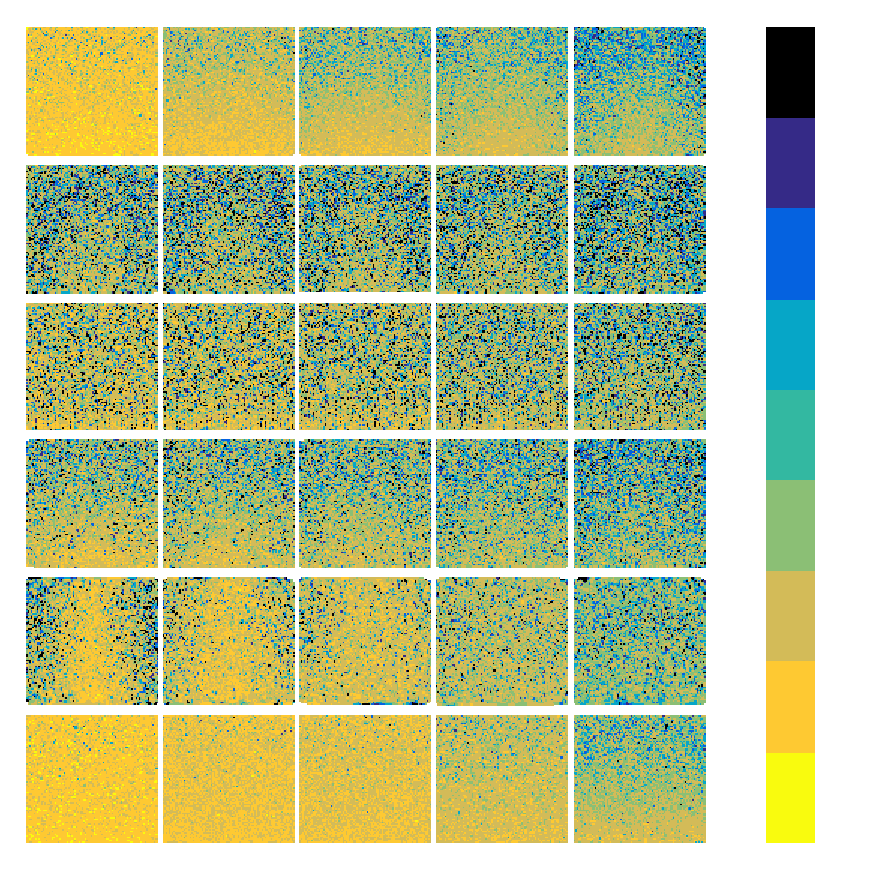
\includegraphics{./figures/parts/appendix/chapters/05/sections/04/caer_style_position_errors_binned_dxyt4}}%
    \gplfronttext
  \end{picture}%
\endgroup

  \vspace{1cm}
  \caption{\small Χάρτες θερμότητας των μέτρων των τελικών σφαλμάτων εκτίμησης
           θέσης συναρτήσει των αρχικών σφαλμάτων εκτίμησης προσανατολισμού
           $\Delta\hat{\theta} \in
           [-\overline{\delta}_{\theta},+\overline{\delta}_{\theta}]$ (στον
           οριζόντιο άξονα) και των μέτρων των αρχικών σφαλμάτων εκτίμησης
           θέσης $\|\Delta \hat{\bm{l}}\|_2 \in [0, \sqrt{2}\cdot
           \overline{\delta}_{xy}]$ (στον κάθετο άξονα) για όλα τα
           διενεργηθέντα πειράματα, ανά αλγόριθμο και ανά τυπική απόκλιση
           διαταραχών του φυσικού αισθητήρα, για τη διάταξη με
           $(\overline{\delta}_{xy}, \overline{\delta}_{\theta}) = (0.20,
           0.30)$ [m,rad]}
  \label{fig:appendix_05_01:04}
\end{figure}
\begin{figure}\vspace{1cm}\hspace{0.5cm}
  % GNUPLOT: LaTeX picture with Postscript
\begingroup
  \makeatletter
  \providecommand\color[2][]{%
    \GenericError{(gnuplot) \space\space\space\@spaces}{%
      Package color not loaded in conjunction with
      terminal option `colourtext'%
    }{See the gnuplot documentation for explanation.%
    }{Either use 'blacktext' in gnuplot or load the package
      color.sty in LaTeX.}%
    \renewcommand\color[2][]{}%
  }%
  \providecommand\includegraphics[2][]{%
    \GenericError{(gnuplot) \space\space\space\@spaces}{%
      Package graphicx or graphics not loaded%
    }{See the gnuplot documentation for explanation.%
    }{The gnuplot epslatex terminal needs graphicx.sty or graphics.sty.}%
    \renewcommand\includegraphics[2][]{}%
  }%
  \providecommand\rotatebox[2]{#2}%
  \@ifundefined{ifGPcolor}{%
    \newif\ifGPcolor
    \GPcolorfalse
  }{}%
  \@ifundefined{ifGPblacktext}{%
    \newif\ifGPblacktext
    \GPblacktexttrue
  }{}%
  % define a \g@addto@macro without @ in the name:
  \let\gplgaddtomacro\g@addto@macro
  % define empty templates for all commands taking text:
  \gdef\gplbacktext{}%
  \gdef\gplfronttext{}%
  \makeatother
  \ifGPblacktext
    % no textcolor at all
    \def\colorrgb#1{}%
    \def\colorgray#1{}%
  \else
    % gray or color?
    \ifGPcolor
      \def\colorrgb#1{\color[rgb]{#1}}%
      \def\colorgray#1{\color[gray]{#1}}%
      \expandafter\def\csname LTw\endcsname{\color{white}}%
      \expandafter\def\csname LTb\endcsname{\color{black}}%
      \expandafter\def\csname LTa\endcsname{\color{black}}%
      \expandafter\def\csname LT0\endcsname{\color[rgb]{1,0,0}}%
      \expandafter\def\csname LT1\endcsname{\color[rgb]{0,1,0}}%
      \expandafter\def\csname LT2\endcsname{\color[rgb]{0,0,1}}%
      \expandafter\def\csname LT3\endcsname{\color[rgb]{1,0,1}}%
      \expandafter\def\csname LT4\endcsname{\color[rgb]{0,1,1}}%
      \expandafter\def\csname LT5\endcsname{\color[rgb]{1,1,0}}%
      \expandafter\def\csname LT6\endcsname{\color[rgb]{0,0,0}}%
      \expandafter\def\csname LT7\endcsname{\color[rgb]{1,0.3,0}}%
      \expandafter\def\csname LT8\endcsname{\color[rgb]{0.5,0.5,0.5}}%
    \else
      % gray
      \def\colorrgb#1{\color{black}}%
      \def\colorgray#1{\color[gray]{#1}}%
      \expandafter\def\csname LTw\endcsname{\color{white}}%
      \expandafter\def\csname LTb\endcsname{\color{black}}%
      \expandafter\def\csname LTa\endcsname{\color{black}}%
      \expandafter\def\csname LT0\endcsname{\color{black}}%
      \expandafter\def\csname LT1\endcsname{\color{black}}%
      \expandafter\def\csname LT2\endcsname{\color{black}}%
      \expandafter\def\csname LT3\endcsname{\color{black}}%
      \expandafter\def\csname LT4\endcsname{\color{black}}%
      \expandafter\def\csname LT5\endcsname{\color{black}}%
      \expandafter\def\csname LT6\endcsname{\color{black}}%
      \expandafter\def\csname LT7\endcsname{\color{black}}%
      \expandafter\def\csname LT8\endcsname{\color{black}}%
    \fi
  \fi
  \setlength{\unitlength}{0.0500bp}%
  \begin{picture}(8000.00,8000.00)%
     \gplgaddtomacro\gplfronttext{%
      \colorrgb{0.00,0.00,0.00}%
      \put(716,8200){\makebox(0,0){\strut{}\small $\sigma_R = 0.01$}}%
      \colorrgb{0.00,0.00,0.00}%
      \put(2029,8200){\makebox(0,0){\strut{}\small $\sigma_R = 0.03$}}%
      \colorrgb{0.00,0.00,0.00}%
      \put(3343,8200){\makebox(0,0){\strut{}\small $\sigma_R = 0.05$}}%
      \colorrgb{0.00,0.00,0.00}%
      \put(4656,8200){\makebox(0,0){\strut{}\small $\sigma_R = 0.10$}}%
      \colorrgb{0.00,0.00,0.00}%
      \put(5969,8200){\makebox(0,0){\strut{}\small $\sigma_R = 0.20$ [m]}}%
      \put(3333.33,8700){\makebox(0,0){\strut{}$(\overline{\delta}_{xy}, \overline{\delta}_\theta) = (0.20 \ \text{m}, 0.56 \ \text{rad})$}}
      \put(4000,9200){\makebox(0,0){\strut{}Τελικά σφάλματα εκτίμησης θέσης ως προς αρχικές συνθήκες μετατόπισης [m]}}
    }%
    \gplgaddtomacro\gplfronttext{%
      \colorrgb{0.00,0.00,0.00}%
      \put(-200,7333.33){\rotatebox{90}{\makebox(0,0){\strut{}\small PLICP}}}%
    }%
    \gplgaddtomacro\gplfronttext{%
      \colorrgb{0.00,0.00,0.00}%
      \put(-200,6000){\rotatebox{90}{\makebox(0,0){\strut{}\small NDT}}}%
    }%
    \gplgaddtomacro\gplfronttext{%
      \colorrgb{0.00,0.00,0.00}%
      \put(-200,4666.66){\rotatebox{90}{\makebox(0,0){\strut{}\small FastGICP}}}%
    }%
    \gplgaddtomacro\gplfronttext{%
      \colorrgb{0.00,0.00,0.00}%
      \put(-200,3333.33){\rotatebox{90}{\makebox(0,0){\strut{}\small FastVGICP}}}%
    }%
    \gplgaddtomacro\gplfronttext{%
      \colorrgb{0.00,0.00,0.00}%
      \put(-200,2000){\rotatebox{90}{\makebox(0,0){\strut{}\small NDT-PSO}}}%
    }%
    \gplgaddtomacro\gplfronttext{%
      \colorrgb{0.00,0.00,0.00}%
      \put(-200,666.66){\rotatebox{90}{\makebox(0,0){\strut{}\small \texttt{fsm}}}}%
    }%
    \gplgaddtomacro\gplfronttext{%
      \colorrgb{0.00,0.00,0.00}%
      \put(7800,515.5){\makebox(0,0)[l]{\strut{}$<0.001$}}%
      \colorrgb{0.00,0.00,0.00}%
      \put(7800,1386.5){\makebox(0,0)[l]{\strut{}$<0.01$}}%
      \colorrgb{0.00,0.0.00,0.00}%
      \put(7800,2257.5){\makebox(0,0)[l]{\strut{}$<0.05$}}%
      \colorrgb{0.00,0.0.00,0.00}%
      \put(7800,3128.5){\makebox(0,0)[l]{\strut{}$<0.1$}}%
      \colorrgb{0.00,0.0.00,0.00}%
      \put(7800,3999.5){\makebox(0,0)[l]{\strut{}$<0.15$}}%
      \colorrgb{0.00,0.0.00,0.00}%
      \put(7800,4870.5){\makebox(0,0)[l]{\strut{}$<0.2$}}%
      \colorrgb{0.00,0.0.00,0.00}%
      \put(7800,5741.5){\makebox(0,0)[l]{\strut{}$<0.25$}}%
      \colorrgb{0.00,0.0.00,0.00}%
      \put(7800,6612.5){\makebox(0,0)[l]{\strut{}$<0.5$}}%
      \colorrgb{0.00,0.00,0.00}%
      \put(7800,7483.5){\makebox(0,0)[l]{\strut{}$<e^{\overline{\delta}_{xy}, \overline{\delta}_\theta}_{xy,\max} = 168.3$}}%
    }%
    \put(0,0){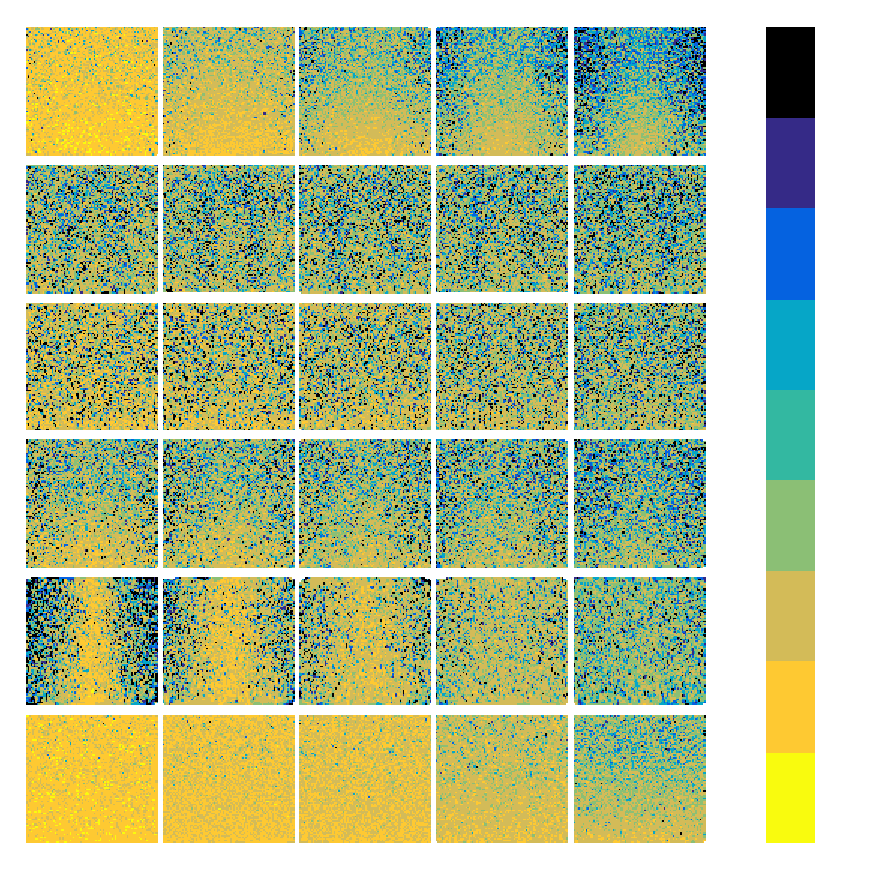
\includegraphics{./figures/parts/appendix/chapters/05/sections/03/caer_style_position_errors_binned_dxyt5}}%
    \gplfronttext
  \end{picture}%
\endgroup

  \vspace{1cm}
  \caption{\small Χάρτες θερμότητας των μέτρων των τελικών σφαλμάτων εκτίμησης
           θέσης συναρτήσει των αρχικών σφαλμάτων εκτίμησης προσανατολισμού
           $\Delta\hat{\theta} \in
           [-\overline{\delta}_{\theta},+\overline{\delta}_{\theta}]$ (στον
           οριζόντιο άξονα) και των μέτρων των αρχικών σφαλμάτων εκτίμησης
           θέσης $\|\Delta \hat{\bm{l}}\|_2 \in [0, \sqrt{2}\cdot
           \overline{\delta}_{xy}]$ (στον κάθετο άξονα) για όλα τα
           διενεργηθέντα πειράματα, ανά αλγόριθμο και ανά τυπική απόκλιση
           διαταραχών του φυσικού αισθητήρα, για τη διάταξη με
           $(\overline{\delta}_{xy}, \overline{\delta}_{\theta}) = (0.20,
           0.56)$ [m,rad]}
  \label{fig:appendix_05_01:05}
\end{figure}
\begin{figure}\vspace{1cm}\hspace{0.5cm}
  % GNUPLOT: LaTeX picture with Postscript
\begingroup
  \makeatletter
  \providecommand\color[2][]{%
    \GenericError{(gnuplot) \space\space\space\@spaces}{%
      Package color not loaded in conjunction with
      terminal option `colourtext'%
    }{See the gnuplot documentation for explanation.%
    }{Either use 'blacktext' in gnuplot or load the package
      color.sty in LaTeX.}%
    \renewcommand\color[2][]{}%
  }%
  \providecommand\includegraphics[2][]{%
    \GenericError{(gnuplot) \space\space\space\@spaces}{%
      Package graphicx or graphics not loaded%
    }{See the gnuplot documentation for explanation.%
    }{The gnuplot epslatex terminal needs graphicx.sty or graphics.sty.}%
    \renewcommand\includegraphics[2][]{}%
  }%
  \providecommand\rotatebox[2]{#2}%
  \@ifundefined{ifGPcolor}{%
    \newif\ifGPcolor
    \GPcolorfalse
  }{}%
  \@ifundefined{ifGPblacktext}{%
    \newif\ifGPblacktext
    \GPblacktexttrue
  }{}%
  % define a \g@addto@macro without @ in the name:
  \let\gplgaddtomacro\g@addto@macro
  % define empty templates for all commands taking text:
  \gdef\gplbacktext{}%
  \gdef\gplfronttext{}%
  \makeatother
  \ifGPblacktext
    % no textcolor at all
    \def\colorrgb#1{}%
    \def\colorgray#1{}%
  \else
    % gray or color?
    \ifGPcolor
      \def\colorrgb#1{\color[rgb]{#1}}%
      \def\colorgray#1{\color[gray]{#1}}%
      \expandafter\def\csname LTw\endcsname{\color{white}}%
      \expandafter\def\csname LTb\endcsname{\color{black}}%
      \expandafter\def\csname LTa\endcsname{\color{black}}%
      \expandafter\def\csname LT0\endcsname{\color[rgb]{1,0,0}}%
      \expandafter\def\csname LT1\endcsname{\color[rgb]{0,1,0}}%
      \expandafter\def\csname LT2\endcsname{\color[rgb]{0,0,1}}%
      \expandafter\def\csname LT3\endcsname{\color[rgb]{1,0,1}}%
      \expandafter\def\csname LT4\endcsname{\color[rgb]{0,1,1}}%
      \expandafter\def\csname LT5\endcsname{\color[rgb]{1,1,0}}%
      \expandafter\def\csname LT6\endcsname{\color[rgb]{0,0,0}}%
      \expandafter\def\csname LT7\endcsname{\color[rgb]{1,0.3,0}}%
      \expandafter\def\csname LT8\endcsname{\color[rgb]{0.5,0.5,0.5}}%
    \else
      % gray
      \def\colorrgb#1{\color{black}}%
      \def\colorgray#1{\color[gray]{#1}}%
      \expandafter\def\csname LTw\endcsname{\color{white}}%
      \expandafter\def\csname LTb\endcsname{\color{black}}%
      \expandafter\def\csname LTa\endcsname{\color{black}}%
      \expandafter\def\csname LT0\endcsname{\color{black}}%
      \expandafter\def\csname LT1\endcsname{\color{black}}%
      \expandafter\def\csname LT2\endcsname{\color{black}}%
      \expandafter\def\csname LT3\endcsname{\color{black}}%
      \expandafter\def\csname LT4\endcsname{\color{black}}%
      \expandafter\def\csname LT5\endcsname{\color{black}}%
      \expandafter\def\csname LT6\endcsname{\color{black}}%
      \expandafter\def\csname LT7\endcsname{\color{black}}%
      \expandafter\def\csname LT8\endcsname{\color{black}}%
    \fi
  \fi
  \setlength{\unitlength}{0.0500bp}%
  \begin{picture}(8000.00,8000.00)%
     \gplgaddtomacro\gplfronttext{%
      \colorrgb{0.00,0.00,0.00}%
      \put(716,8200){\makebox(0,0){\strut{}\small $\sigma_R = 0.01$}}%
      \colorrgb{0.00,0.00,0.00}%
      \put(2029,8200){\makebox(0,0){\strut{}\small $\sigma_R = 0.03$}}%
      \colorrgb{0.00,0.00,0.00}%
      \put(3343,8200){\makebox(0,0){\strut{}\small $\sigma_R = 0.05$}}%
      \colorrgb{0.00,0.00,0.00}%
      \put(4656,8200){\makebox(0,0){\strut{}\small $\sigma_R = 0.10$}}%
      \colorrgb{0.00,0.00,0.00}%
      \put(5969,8200){\makebox(0,0){\strut{}\small $\sigma_R = 0.20$ [m]}}%
      \put(3333.33,8700){\makebox(0,0){\strut{}$(\overline{\delta}_{xy}, \overline{\delta}_\theta) = (0.20 \ \text{m}, \pi/4 \ \text{rad})$}}
      \put(4000,9200){\makebox(0,0){\strut{}Τελικά σφάλματα εκτίμησης θέσης ως προς αρχικές συνθήκες μετατόπισης [m]}}
    }%
    \gplgaddtomacro\gplfronttext{%
      \colorrgb{0.00,0.00,0.00}%
      \put(-200,7333.33){\rotatebox{90}{\makebox(0,0){\strut{}\small PLICP}}}%
    }%
    \gplgaddtomacro\gplfronttext{%
      \colorrgb{0.00,0.00,0.00}%
      \put(-200,6000){\rotatebox{90}{\makebox(0,0){\strut{}\small NDT}}}%
    }%
    \gplgaddtomacro\gplfronttext{%
      \colorrgb{0.00,0.00,0.00}%
      \put(-200,4666.66){\rotatebox{90}{\makebox(0,0){\strut{}\small FastGICP}}}%
    }%
    \gplgaddtomacro\gplfronttext{%
      \colorrgb{0.00,0.00,0.00}%
      \put(-200,3333.33){\rotatebox{90}{\makebox(0,0){\strut{}\small FastVGICP}}}%
    }%
    \gplgaddtomacro\gplfronttext{%
      \colorrgb{0.00,0.00,0.00}%
      \put(-200,2000){\rotatebox{90}{\makebox(0,0){\strut{}\small NDT-PSO}}}%
    }%
    \gplgaddtomacro\gplfronttext{%
      \colorrgb{0.00,0.00,0.00}%
      \put(-200,666.66){\rotatebox{90}{\makebox(0,0){\strut{}\small \texttt{fsm}}}}%
    }%
    \gplgaddtomacro\gplfronttext{%
      \colorrgb{0.00,0.00,0.00}%
      \put(7800,515.5){\makebox(0,0)[l]{\strut{}$<0.001$}}%
      \colorrgb{0.00,0.00,0.00}%
      \put(7800,1386.5){\makebox(0,0)[l]{\strut{}$<0.01$}}%
      \colorrgb{0.00,0.0.00,0.00}%
      \put(7800,2257.5){\makebox(0,0)[l]{\strut{}$<0.05$}}%
      \colorrgb{0.00,0.0.00,0.00}%
      \put(7800,3128.5){\makebox(0,0)[l]{\strut{}$<0.1$}}%
      \colorrgb{0.00,0.0.00,0.00}%
      \put(7800,3999.5){\makebox(0,0)[l]{\strut{}$<0.15$}}%
      \colorrgb{0.00,0.0.00,0.00}%
      \put(7800,4870.5){\makebox(0,0)[l]{\strut{}$<0.2$}}%
      \colorrgb{0.00,0.0.00,0.00}%
      \put(7800,5741.5){\makebox(0,0)[l]{\strut{}$<0.25$}}%
      \colorrgb{0.00,0.0.00,0.00}%
      \put(7800,6612.5){\makebox(0,0)[l]{\strut{}$<0.5$}}%
      \colorrgb{0.00,0.00,0.00}%
      \put(7800,7483.5){\makebox(0,0)[l]{\strut{}$<e^{\overline{\delta}_{xy}, \overline{\delta}_\theta}_{xy,\max} = 159.3$}}%
    }%
    \put(0,0){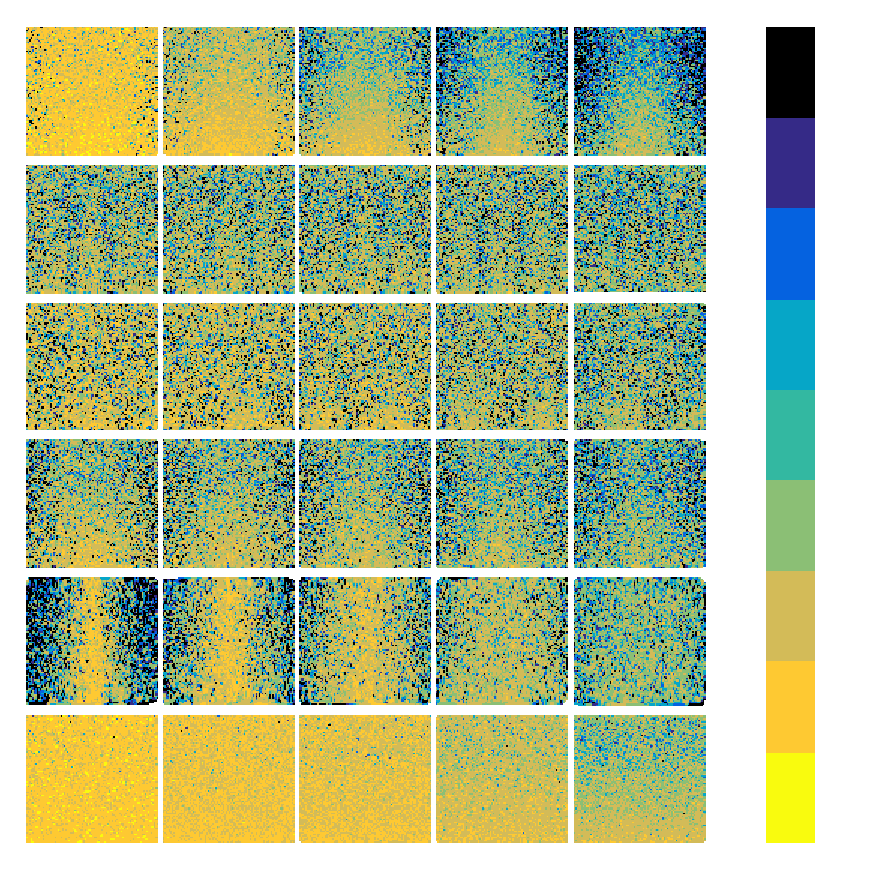
\includegraphics{./figures/parts/02/chapters/05/sections/04/caer_style_position_errors_binned_dxyt6}}%
    \gplfronttext
  \end{picture}%
\endgroup

  \vspace{1cm}
  \caption{\small Χάρτες θερμότητας των μέτρων των τελικών σφαλμάτων εκτίμησης
           θέσης συναρτήσει των αρχικών σφαλμάτων εκτίμησης προσανατολισμού
           $\Delta\hat{\theta} \in
           [-\overline{\delta}_{\theta},+\overline{\delta}_{\theta}]$ (στον
           οριζόντιο άξονα) και των μέτρων των αρχικών σφαλμάτων εκτίμησης
           θέσης $\|\Delta \hat{\bm{l}}\|_2 \in [0, \sqrt{2}\cdot
           \overline{\delta}_{xy}]$ (στον κάθετο άξονα) για όλα τα
           διενεργηθέντα πειράματα, ανά αλγόριθμο και ανά τυπική απόκλιση
           διαταραχών του φυσικού αισθητήρα, για τη διάταξη με
           $(\overline{\delta}_{xy}, \overline{\delta}_{\theta}) = (0.20,
           \pi/4)$ [m,rad]}
  \label{fig:appendix_05_01:06}
\end{figure}


\begin{figure}\vspace{1cm}\hspace{0.5cm}
  % GNUPLOT: LaTeX picture with Postscript
\begingroup
  \makeatletter
  \providecommand\color[2][]{%
    \GenericError{(gnuplot) \space\space\space\@spaces}{%
      Package color not loaded in conjunction with
      terminal option `colourtext'%
    }{See the gnuplot documentation for explanation.%
    }{Either use 'blacktext' in gnuplot or load the package
      color.sty in LaTeX.}%
    \renewcommand\color[2][]{}%
  }%
  \providecommand\includegraphics[2][]{%
    \GenericError{(gnuplot) \space\space\space\@spaces}{%
      Package graphicx or graphics not loaded%
    }{See the gnuplot documentation for explanation.%
    }{The gnuplot epslatex terminal needs graphicx.sty or graphics.sty.}%
    \renewcommand\includegraphics[2][]{}%
  }%
  \providecommand\rotatebox[2]{#2}%
  \@ifundefined{ifGPcolor}{%
    \newif\ifGPcolor
    \GPcolorfalse
  }{}%
  \@ifundefined{ifGPblacktext}{%
    \newif\ifGPblacktext
    \GPblacktexttrue
  }{}%
  % define a \g@addto@macro without @ in the name:
  \let\gplgaddtomacro\g@addto@macro
  % define empty templates for all commands taking text:
  \gdef\gplbacktext{}%
  \gdef\gplfronttext{}%
  \makeatother
  \ifGPblacktext
    % no textcolor at all
    \def\colorrgb#1{}%
    \def\colorgray#1{}%
  \else
    % gray or color?
    \ifGPcolor
      \def\colorrgb#1{\color[rgb]{#1}}%
      \def\colorgray#1{\color[gray]{#1}}%
      \expandafter\def\csname LTw\endcsname{\color{white}}%
      \expandafter\def\csname LTb\endcsname{\color{black}}%
      \expandafter\def\csname LTa\endcsname{\color{black}}%
      \expandafter\def\csname LT0\endcsname{\color[rgb]{1,0,0}}%
      \expandafter\def\csname LT1\endcsname{\color[rgb]{0,1,0}}%
      \expandafter\def\csname LT2\endcsname{\color[rgb]{0,0,1}}%
      \expandafter\def\csname LT3\endcsname{\color[rgb]{1,0,1}}%
      \expandafter\def\csname LT4\endcsname{\color[rgb]{0,1,1}}%
      \expandafter\def\csname LT5\endcsname{\color[rgb]{1,1,0}}%
      \expandafter\def\csname LT6\endcsname{\color[rgb]{0,0,0}}%
      \expandafter\def\csname LT7\endcsname{\color[rgb]{1,0.3,0}}%
      \expandafter\def\csname LT8\endcsname{\color[rgb]{0.5,0.5,0.5}}%
    \else
      % gray
      \def\colorrgb#1{\color{black}}%
      \def\colorgray#1{\color[gray]{#1}}%
      \expandafter\def\csname LTw\endcsname{\color{white}}%
      \expandafter\def\csname LTb\endcsname{\color{black}}%
      \expandafter\def\csname LTa\endcsname{\color{black}}%
      \expandafter\def\csname LT0\endcsname{\color{black}}%
      \expandafter\def\csname LT1\endcsname{\color{black}}%
      \expandafter\def\csname LT2\endcsname{\color{black}}%
      \expandafter\def\csname LT3\endcsname{\color{black}}%
      \expandafter\def\csname LT4\endcsname{\color{black}}%
      \expandafter\def\csname LT5\endcsname{\color{black}}%
      \expandafter\def\csname LT6\endcsname{\color{black}}%
      \expandafter\def\csname LT7\endcsname{\color{black}}%
      \expandafter\def\csname LT8\endcsname{\color{black}}%
    \fi
  \fi
  \setlength{\unitlength}{0.0500bp}%
  \begin{picture}(8000.00,8000.00)%
     \gplgaddtomacro\gplfronttext{%
      \colorrgb{0.00,0.00,0.00}%
      \put(716,8200){\makebox(0,0){\strut{}\small $\sigma_R = 0.01$}}%
      \colorrgb{0.00,0.00,0.00}%
      \put(2029,8200){\makebox(0,0){\strut{}\small $\sigma_R = 0.03$}}%
      \colorrgb{0.00,0.00,0.00}%
      \put(3343,8200){\makebox(0,0){\strut{}\small $\sigma_R = 0.05$}}%
      \colorrgb{0.00,0.00,0.00}%
      \put(4656,8200){\makebox(0,0){\strut{}\small $\sigma_R = 0.10$}}%
      \colorrgb{0.00,0.00,0.00}%
      \put(5969,8200){\makebox(0,0){\strut{}\small $\sigma_R = 0.20$ [m]}}%
    }%
    \gplgaddtomacro\gplfronttext{%
      \colorrgb{0.00,0.00,0.00}%
      \put(-200,7333.33){\rotatebox{90}{\makebox(0,0){\strut{}\small PLICP}}}%
    }%
    \gplgaddtomacro\gplfronttext{%
      \colorrgb{0.00,0.00,0.00}%
      \put(-200,6000){\rotatebox{90}{\makebox(0,0){\strut{}\small NDT}}}%
    }%
    \gplgaddtomacro\gplfronttext{%
      \colorrgb{0.00,0.00,0.00}%
      \put(-200,4666.66){\rotatebox{90}{\makebox(0,0){\strut{}\small FastGICP}}}%
    }%
    \gplgaddtomacro\gplfronttext{%
      \colorrgb{0.00,0.00,0.00}%
      \put(-200,3333.33){\rotatebox{90}{\makebox(0,0){\strut{}\small FastVGICP}}}%
    }%
    \gplgaddtomacro\gplfronttext{%
      \colorrgb{0.00,0.00,0.00}%
      \put(-200,2000){\rotatebox{90}{\makebox(0,0){\strut{}\small NDT-PSO}}}%
    }%
    \gplgaddtomacro\gplfronttext{%
      \colorrgb{0.00,0.00,0.00}%
      \put(-200,666.66){\rotatebox{90}{\makebox(0,0){\strut{}\small \texttt{fsm}}}}%
    }%
    \gplgaddtomacro\gplfronttext{%
      \colorrgb{0.00,0.00,0.00}%
      \put(7800,515.5){\makebox(0,0)[l]{\strut{}$<0.001$}}%
      \colorrgb{0.00,0.00,0.00}%
      \put(7800,1386.5){\makebox(0,0)[l]{\strut{}$<0.01$}}%
      \colorrgb{0.00,0.00,0.00}%
      \put(7800,2257.5){\makebox(0,0)[l]{\strut{}$<0.02$}}%
      \colorrgb{0.00,0.00,0.00}%
      \put(7800,3128.5){\makebox(0,0)[l]{\strut{}$<0.05$}}%
      \colorrgb{0.00,0.00,0.00}%
      \put(7800,3999.5){\makebox(0,0)[l]{\strut{}$<0.1$}}%
      \colorrgb{0.00,0.00,0.00}%
      \put(7800,4870.5){\makebox(0,0)[l]{\strut{}$<0.2$}}%
      \colorrgb{0.00,0.00,0.00}%
      \put(7800,5741.5){\makebox(0,0)[l]{\strut{}$<0.5$}}%
      \colorrgb{0.00,0.00,0.00}%
      \put(7800,6612.5){\makebox(0,0)[l]{\strut{}$<1$}}%
      \colorrgb{0.00,0.00,0.00}%
      \put(7800,7483.5){\makebox(0,0)[l]{\strut{}$<2.9473$}}%
    }%
    \put(0,0){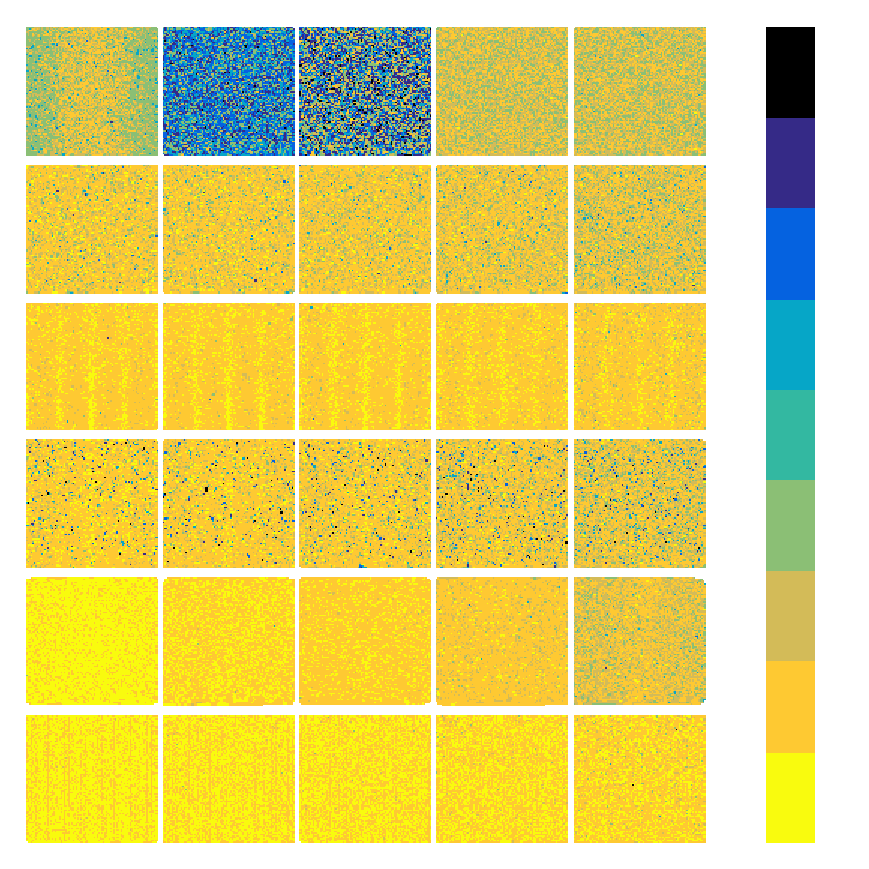
\includegraphics{./figures/parts/appendix/chapters/05/sections/04/caer_style_orientation_errors_binned_dxyt1}}%
    \gplfronttext
  \end{picture}%
\endgroup

  \vspace{1cm}
  \caption{\small Χάρτες θερμότητας των μέτρων των τελικών σφαλμάτων εκτίμησης
           προσανατολισμού συναρτήσει των αρχικών σφαλμάτων εκτίμησης
           προσανατολισμού $\Delta\hat{\theta} \in
           [-\overline{\delta}_{\theta},+\overline{\delta}_{\theta}]$ (στον
           οριζόντιο άξονα) και των μέτρων των αρχικών σφαλμάτων εκτίμησης
           θέσης $\|\Delta \hat{\bm{l}}\|_2 \in [0, \sqrt{2}\cdot
           \overline{\delta}_{xy}]$ (στον κάθετο άξονα) για όλα τα
           διενεργηθέντα πειράματα, ανά αλγόριθμο και ανά τυπική απόκλιση
           διαταραχών του φυσικού αισθητήρα, για τη διάταξη με
           $(\overline{\delta}_{xy}, \overline{\delta}_{\theta}) = (0.05,
           0.035)$ [m,rad]}
  \label{fig:appendix_05_01:07}
\end{figure}
\begin{figure}\vspace{1cm}\hspace{0.5cm}
  % GNUPLOT: LaTeX picture with Postscript
\begingroup
  \makeatletter
  \providecommand\color[2][]{%
    \GenericError{(gnuplot) \space\space\space\@spaces}{%
      Package color not loaded in conjunction with
      terminal option `colourtext'%
    }{See the gnuplot documentation for explanation.%
    }{Either use 'blacktext' in gnuplot or load the package
      color.sty in LaTeX.}%
    \renewcommand\color[2][]{}%
  }%
  \providecommand\includegraphics[2][]{%
    \GenericError{(gnuplot) \space\space\space\@spaces}{%
      Package graphicx or graphics not loaded%
    }{See the gnuplot documentation for explanation.%
    }{The gnuplot epslatex terminal needs graphicx.sty or graphics.sty.}%
    \renewcommand\includegraphics[2][]{}%
  }%
  \providecommand\rotatebox[2]{#2}%
  \@ifundefined{ifGPcolor}{%
    \newif\ifGPcolor
    \GPcolorfalse
  }{}%
  \@ifundefined{ifGPblacktext}{%
    \newif\ifGPblacktext
    \GPblacktexttrue
  }{}%
  % define a \g@addto@macro without @ in the name:
  \let\gplgaddtomacro\g@addto@macro
  % define empty templates for all commands taking text:
  \gdef\gplbacktext{}%
  \gdef\gplfronttext{}%
  \makeatother
  \ifGPblacktext
    % no textcolor at all
    \def\colorrgb#1{}%
    \def\colorgray#1{}%
  \else
    % gray or color?
    \ifGPcolor
      \def\colorrgb#1{\color[rgb]{#1}}%
      \def\colorgray#1{\color[gray]{#1}}%
      \expandafter\def\csname LTw\endcsname{\color{white}}%
      \expandafter\def\csname LTb\endcsname{\color{black}}%
      \expandafter\def\csname LTa\endcsname{\color{black}}%
      \expandafter\def\csname LT0\endcsname{\color[rgb]{1,0,0}}%
      \expandafter\def\csname LT1\endcsname{\color[rgb]{0,1,0}}%
      \expandafter\def\csname LT2\endcsname{\color[rgb]{0,0,1}}%
      \expandafter\def\csname LT3\endcsname{\color[rgb]{1,0,1}}%
      \expandafter\def\csname LT4\endcsname{\color[rgb]{0,1,1}}%
      \expandafter\def\csname LT5\endcsname{\color[rgb]{1,1,0}}%
      \expandafter\def\csname LT6\endcsname{\color[rgb]{0,0,0}}%
      \expandafter\def\csname LT7\endcsname{\color[rgb]{1,0.3,0}}%
      \expandafter\def\csname LT8\endcsname{\color[rgb]{0.5,0.5,0.5}}%
    \else
      % gray
      \def\colorrgb#1{\color{black}}%
      \def\colorgray#1{\color[gray]{#1}}%
      \expandafter\def\csname LTw\endcsname{\color{white}}%
      \expandafter\def\csname LTb\endcsname{\color{black}}%
      \expandafter\def\csname LTa\endcsname{\color{black}}%
      \expandafter\def\csname LT0\endcsname{\color{black}}%
      \expandafter\def\csname LT1\endcsname{\color{black}}%
      \expandafter\def\csname LT2\endcsname{\color{black}}%
      \expandafter\def\csname LT3\endcsname{\color{black}}%
      \expandafter\def\csname LT4\endcsname{\color{black}}%
      \expandafter\def\csname LT5\endcsname{\color{black}}%
      \expandafter\def\csname LT6\endcsname{\color{black}}%
      \expandafter\def\csname LT7\endcsname{\color{black}}%
      \expandafter\def\csname LT8\endcsname{\color{black}}%
    \fi
  \fi
  \setlength{\unitlength}{0.0500bp}%
  \begin{picture}(8000.00,8000.00)%
     \gplgaddtomacro\gplfronttext{%
      \colorrgb{0.00,0.00,0.00}%
      \put(716,8200){\makebox(0,0){\strut{}\small $\sigma_R = 0.01$}}%
      \colorrgb{0.00,0.00,0.00}%
      \put(2029,8200){\makebox(0,0){\strut{}\small $\sigma_R = 0.03$}}%
      \colorrgb{0.00,0.00,0.00}%
      \put(3343,8200){\makebox(0,0){\strut{}\small $\sigma_R = 0.05$}}%
      \colorrgb{0.00,0.00,0.00}%
      \put(4656,8200){\makebox(0,0){\strut{}\small $\sigma_R = 0.10$}}%
      \colorrgb{0.00,0.00,0.00}%
      \put(5969,8200){\makebox(0,0){\strut{}\small $\sigma_R = 0.20$ [m]}}%
      \put(3333.33,8700){\makebox(0,0){\strut{}$(\overline{\delta}_{xy}, \overline{\delta}_\theta) = (0.10 \ \text{m}, 0.07 \ \text{rad})$}}
      \put(4000,9200){\makebox(0,0){\strut{}Τελικά σφάλματα εκτίμησης προσανατολισμού ως προς αρχικές συνθήκες μετατόπισης [rad]}}
    }%
    \gplgaddtomacro\gplfronttext{%
      \colorrgb{0.00,0.00,0.00}%
      \put(-200,7333.33){\rotatebox{90}{\makebox(0,0){\strut{}\small PLICP}}}%
    }%
    \gplgaddtomacro\gplfronttext{%
      \colorrgb{0.00,0.00,0.00}%
      \put(-200,6000){\rotatebox{90}{\makebox(0,0){\strut{}\small NDT}}}%
    }%
    \gplgaddtomacro\gplfronttext{%
      \colorrgb{0.00,0.00,0.00}%
      \put(-200,4666.66){\rotatebox{90}{\makebox(0,0){\strut{}\small FastGICP}}}%
    }%
    \gplgaddtomacro\gplfronttext{%
      \colorrgb{0.00,0.00,0.00}%
      \put(-200,3333.33){\rotatebox{90}{\makebox(0,0){\strut{}\small FastVGICP}}}%
    }%
    \gplgaddtomacro\gplfronttext{%
      \colorrgb{0.00,0.00,0.00}%
      \put(-200,2000){\rotatebox{90}{\makebox(0,0){\strut{}\small NDT-PSO}}}%
    }%
    \gplgaddtomacro\gplfronttext{%
      \colorrgb{0.00,0.00,0.00}%
      \put(-200,666.66){\rotatebox{90}{\makebox(0,0){\strut{}\small \texttt{fsm}}}}%
    }%
    \gplgaddtomacro\gplfronttext{%
      \colorrgb{0.00,0.00,0.00}%
      \put(7800,515.5){\makebox(0,0)[l]{\strut{}$<0.001$}}%
      \colorrgb{0.00,0.00,0.00}%
      \put(7800,1386.5){\makebox(0,0)[l]{\strut{}$<0.01$}}%
      \colorrgb{0.00,0.00,0.00}%
      \put(7800,2257.5){\makebox(0,0)[l]{\strut{}$<0.02$}}%
      \colorrgb{0.00,0.00,0.00}%
      \put(7800,3128.5){\makebox(0,0)[l]{\strut{}$<0.05$}}%
      \colorrgb{0.00,0.00,0.00}%
      \put(7800,3999.5){\makebox(0,0)[l]{\strut{}$<0.1$}}%
      \colorrgb{0.00,0.00,0.00}%
      \put(7800,4870.5){\makebox(0,0)[l]{\strut{}$<0.2$}}%
      \colorrgb{0.00,0.00,0.00}%
      \put(7800,5741.5){\makebox(0,0)[l]{\strut{}$<0.5$}}%
      \colorrgb{0.00,0.00,0.00}%
      \put(7800,6612.5){\makebox(0,0)[l]{\strut{}$<1$}}%
      \colorrgb{0.00,0.00,0.00}%
      \put(7800,7483.5){\makebox(0,0)[l]{\strut{}$<e^{\overline{\delta}_{xy}, \overline{\delta}_\theta}_{\theta,\max} = 2.912$}}%
    }%
    \put(0,0){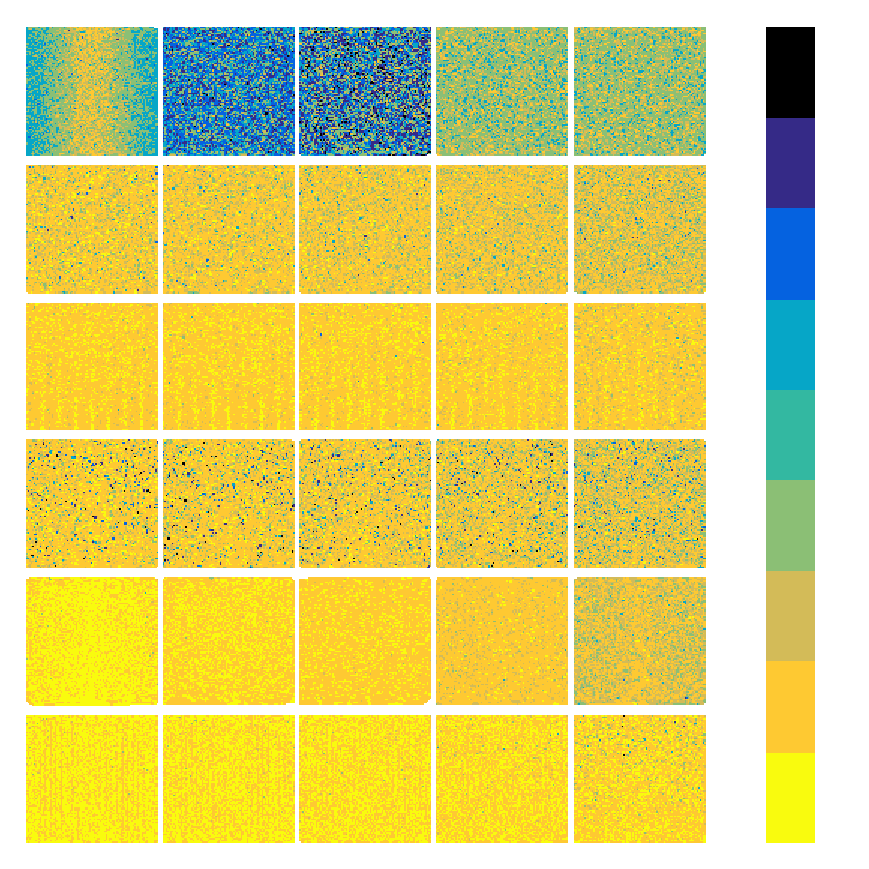
\includegraphics{./figures/parts/appendix/chapters/05/sections/04/caer_style_orientation_errors_binned_dxyt2}}%
    \gplfronttext
  \end{picture}%
\endgroup

  \vspace{1cm}
  \caption{\small Χάρτες θερμότητας των μέτρων των τελικών σφαλμάτων εκτίμησης
           προσανατολισμού συναρτήσει των αρχικών σφαλμάτων εκτίμησης
           προσανατολισμού $\Delta\hat{\theta} \in
           [-\overline{\delta}_{\theta},+\overline{\delta}_{\theta}]$ (στον
           οριζόντιο άξονα) και των μέτρων των αρχικών σφαλμάτων εκτίμησης
           θέσης $\|\Delta \hat{\bm{l}}\|_2 \in [0, \sqrt{2}\cdot
           \overline{\delta}_{xy}]$ (στον κάθετο άξονα) για όλα τα
           διενεργηθέντα πειράματα, ανά αλγόριθμο και ανά τυπική απόκλιση
           διαταραχών του φυσικού αισθητήρα, για τη διάταξη με
           $(\overline{\delta}_{xy}, \overline{\delta}_{\theta}) = (0.10,
           0.070)$ [m,rad]}
  \label{fig:appendix_05_01:08}
\end{figure}
\begin{figure}\vspace{1cm}\hspace{0.5cm}
  % GNUPLOT: LaTeX picture with Postscript
\begingroup
  \makeatletter
  \providecommand\color[2][]{%
    \GenericError{(gnuplot) \space\space\space\@spaces}{%
      Package color not loaded in conjunction with
      terminal option `colourtext'%
    }{See the gnuplot documentation for explanation.%
    }{Either use 'blacktext' in gnuplot or load the package
      color.sty in LaTeX.}%
    \renewcommand\color[2][]{}%
  }%
  \providecommand\includegraphics[2][]{%
    \GenericError{(gnuplot) \space\space\space\@spaces}{%
      Package graphicx or graphics not loaded%
    }{See the gnuplot documentation for explanation.%
    }{The gnuplot epslatex terminal needs graphicx.sty or graphics.sty.}%
    \renewcommand\includegraphics[2][]{}%
  }%
  \providecommand\rotatebox[2]{#2}%
  \@ifundefined{ifGPcolor}{%
    \newif\ifGPcolor
    \GPcolorfalse
  }{}%
  \@ifundefined{ifGPblacktext}{%
    \newif\ifGPblacktext
    \GPblacktexttrue
  }{}%
  % define a \g@addto@macro without @ in the name:
  \let\gplgaddtomacro\g@addto@macro
  % define empty templates for all commands taking text:
  \gdef\gplbacktext{}%
  \gdef\gplfronttext{}%
  \makeatother
  \ifGPblacktext
    % no textcolor at all
    \def\colorrgb#1{}%
    \def\colorgray#1{}%
  \else
    % gray or color?
    \ifGPcolor
      \def\colorrgb#1{\color[rgb]{#1}}%
      \def\colorgray#1{\color[gray]{#1}}%
      \expandafter\def\csname LTw\endcsname{\color{white}}%
      \expandafter\def\csname LTb\endcsname{\color{black}}%
      \expandafter\def\csname LTa\endcsname{\color{black}}%
      \expandafter\def\csname LT0\endcsname{\color[rgb]{1,0,0}}%
      \expandafter\def\csname LT1\endcsname{\color[rgb]{0,1,0}}%
      \expandafter\def\csname LT2\endcsname{\color[rgb]{0,0,1}}%
      \expandafter\def\csname LT3\endcsname{\color[rgb]{1,0,1}}%
      \expandafter\def\csname LT4\endcsname{\color[rgb]{0,1,1}}%
      \expandafter\def\csname LT5\endcsname{\color[rgb]{1,1,0}}%
      \expandafter\def\csname LT6\endcsname{\color[rgb]{0,0,0}}%
      \expandafter\def\csname LT7\endcsname{\color[rgb]{1,0.3,0}}%
      \expandafter\def\csname LT8\endcsname{\color[rgb]{0.5,0.5,0.5}}%
    \else
      % gray
      \def\colorrgb#1{\color{black}}%
      \def\colorgray#1{\color[gray]{#1}}%
      \expandafter\def\csname LTw\endcsname{\color{white}}%
      \expandafter\def\csname LTb\endcsname{\color{black}}%
      \expandafter\def\csname LTa\endcsname{\color{black}}%
      \expandafter\def\csname LT0\endcsname{\color{black}}%
      \expandafter\def\csname LT1\endcsname{\color{black}}%
      \expandafter\def\csname LT2\endcsname{\color{black}}%
      \expandafter\def\csname LT3\endcsname{\color{black}}%
      \expandafter\def\csname LT4\endcsname{\color{black}}%
      \expandafter\def\csname LT5\endcsname{\color{black}}%
      \expandafter\def\csname LT6\endcsname{\color{black}}%
      \expandafter\def\csname LT7\endcsname{\color{black}}%
      \expandafter\def\csname LT8\endcsname{\color{black}}%
    \fi
  \fi
  \setlength{\unitlength}{0.0500bp}%
  \begin{picture}(8000.00,8000.00)%
     \gplgaddtomacro\gplfronttext{%
      \colorrgb{0.00,0.00,0.00}%
      \put(716,8200){\makebox(0,0){\strut{}\small $\sigma_R = 0.01$}}%
      \colorrgb{0.00,0.00,0.00}%
      \put(2029,8200){\makebox(0,0){\strut{}\small $\sigma_R = 0.03$}}%
      \colorrgb{0.00,0.00,0.00}%
      \put(3343,8200){\makebox(0,0){\strut{}\small $\sigma_R = 0.05$}}%
      \colorrgb{0.00,0.00,0.00}%
      \put(4656,8200){\makebox(0,0){\strut{}\small $\sigma_R = 0.10$}}%
      \colorrgb{0.00,0.00,0.00}%
      \put(5969,8200){\makebox(0,0){\strut{}\small $\sigma_R = 0.20$ [m]}}%
    }%
    \gplgaddtomacro\gplfronttext{%
      \colorrgb{0.00,0.00,0.00}%
      \put(-200,7333.33){\rotatebox{90}{\makebox(0,0){\strut{}\small PLICP}}}%
    }%
    \gplgaddtomacro\gplfronttext{%
      \colorrgb{0.00,0.00,0.00}%
      \put(-200,6000){\rotatebox{90}{\makebox(0,0){\strut{}\small NDT}}}%
    }%
    \gplgaddtomacro\gplfronttext{%
      \colorrgb{0.00,0.00,0.00}%
      \put(-200,4666.66){\rotatebox{90}{\makebox(0,0){\strut{}\small FastGICP}}}%
    }%
    \gplgaddtomacro\gplfronttext{%
      \colorrgb{0.00,0.00,0.00}%
      \put(-200,3333.33){\rotatebox{90}{\makebox(0,0){\strut{}\small FastVGICP}}}%
    }%
    \gplgaddtomacro\gplfronttext{%
      \colorrgb{0.00,0.00,0.00}%
      \put(-200,2000){\rotatebox{90}{\makebox(0,0){\strut{}\small NDT-PSO}}}%
    }%
    \gplgaddtomacro\gplfronttext{%
      \colorrgb{0.00,0.00,0.00}%
      \put(-200,666.66){\rotatebox{90}{\makebox(0,0){\strut{}\small \texttt{fsm}}}}%
    }%
    \gplgaddtomacro\gplfronttext{%
      \colorrgb{0.00,0.00,0.00}%
      \put(7800,515.5){\makebox(0,0)[l]{\strut{}$<0.001$}}%
      \colorrgb{0.00,0.00,0.00}%
      \put(7800,1386.5){\makebox(0,0)[l]{\strut{}$<0.01$}}%
      \colorrgb{0.00,0.00,0.00}%
      \put(7800,2257.5){\makebox(0,0)[l]{\strut{}$<0.02$}}%
      \colorrgb{0.00,0.00,0.00}%
      \put(7800,3128.5){\makebox(0,0)[l]{\strut{}$<0.05$}}%
      \colorrgb{0.00,0.00,0.00}%
      \put(7800,3999.5){\makebox(0,0)[l]{\strut{}$<0.1$}}%
      \colorrgb{0.00,0.00,0.00}%
      \put(7800,4870.5){\makebox(0,0)[l]{\strut{}$<0.2$}}%
      \colorrgb{0.00,0.00,0.00}%
      \put(7800,5741.5){\makebox(0,0)[l]{\strut{}$<0.5$}}%
      \colorrgb{0.00,0.00,0.00}%
      \put(7800,6612.5){\makebox(0,0)[l]{\strut{}$<1$}}%
      \colorrgb{0.00,0.00,0.00}%
      \put(7800,7483.5){\makebox(0,0)[l]{\strut{}$<2.8697$}}%
    }%
    \put(0,0){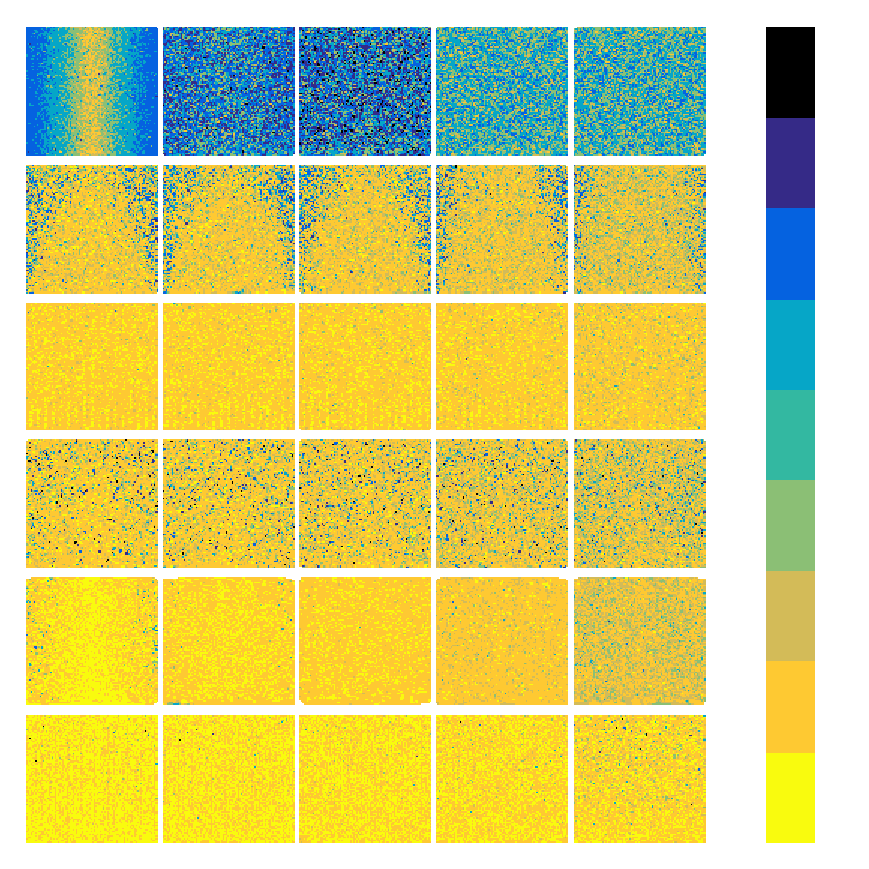
\includegraphics{./figures/parts/appendix/chapters/05/sections/04/caer_style_orientation_errors_binned_dxyt3}}%
    \gplfronttext
  \end{picture}%
\endgroup

  \vspace{1cm}
  \caption{\small Χάρτες θερμότητας των μέτρων των τελικών σφαλμάτων εκτίμησης
           προσανατολισμού συναρτήσει των αρχικών σφαλμάτων εκτίμησης
           προσανατολισμού $\Delta\hat{\theta} \in
           [-\overline{\delta}_{\theta},+\overline{\delta}_{\theta}]$ (στον
           οριζόντιο άξονα) και των μέτρων των αρχικών σφαλμάτων εκτίμησης
           θέσης $\|\Delta \hat{\bm{l}}\|_2 \in [0, \sqrt{2}\cdot
           \overline{\delta}_{xy}]$ (στον κάθετο άξονα) για όλα τα
           διενεργηθέντα πειράματα, ανά αλγόριθμο και ανά τυπική απόκλιση
           διαταραχών του φυσικού αισθητήρα, για τη διάταξη με
           $(\overline{\delta}_{xy}, \overline{\delta}_{\theta}) = (0.15,
           0.150)$ [m,rad]}
  \label{fig:appendix_05_01:09}
\end{figure}
\begin{figure}\vspace{1cm}\hspace{0.5cm}
  % GNUPLOT: LaTeX picture with Postscript
\begingroup
  \makeatletter
  \providecommand\color[2][]{%
    \GenericError{(gnuplot) \space\space\space\@spaces}{%
      Package color not loaded in conjunction with
      terminal option `colourtext'%
    }{See the gnuplot documentation for explanation.%
    }{Either use 'blacktext' in gnuplot or load the package
      color.sty in LaTeX.}%
    \renewcommand\color[2][]{}%
  }%
  \providecommand\includegraphics[2][]{%
    \GenericError{(gnuplot) \space\space\space\@spaces}{%
      Package graphicx or graphics not loaded%
    }{See the gnuplot documentation for explanation.%
    }{The gnuplot epslatex terminal needs graphicx.sty or graphics.sty.}%
    \renewcommand\includegraphics[2][]{}%
  }%
  \providecommand\rotatebox[2]{#2}%
  \@ifundefined{ifGPcolor}{%
    \newif\ifGPcolor
    \GPcolorfalse
  }{}%
  \@ifundefined{ifGPblacktext}{%
    \newif\ifGPblacktext
    \GPblacktexttrue
  }{}%
  % define a \g@addto@macro without @ in the name:
  \let\gplgaddtomacro\g@addto@macro
  % define empty templates for all commands taking text:
  \gdef\gplbacktext{}%
  \gdef\gplfronttext{}%
  \makeatother
  \ifGPblacktext
    % no textcolor at all
    \def\colorrgb#1{}%
    \def\colorgray#1{}%
  \else
    % gray or color?
    \ifGPcolor
      \def\colorrgb#1{\color[rgb]{#1}}%
      \def\colorgray#1{\color[gray]{#1}}%
      \expandafter\def\csname LTw\endcsname{\color{white}}%
      \expandafter\def\csname LTb\endcsname{\color{black}}%
      \expandafter\def\csname LTa\endcsname{\color{black}}%
      \expandafter\def\csname LT0\endcsname{\color[rgb]{1,0,0}}%
      \expandafter\def\csname LT1\endcsname{\color[rgb]{0,1,0}}%
      \expandafter\def\csname LT2\endcsname{\color[rgb]{0,0,1}}%
      \expandafter\def\csname LT3\endcsname{\color[rgb]{1,0,1}}%
      \expandafter\def\csname LT4\endcsname{\color[rgb]{0,1,1}}%
      \expandafter\def\csname LT5\endcsname{\color[rgb]{1,1,0}}%
      \expandafter\def\csname LT6\endcsname{\color[rgb]{0,0,0}}%
      \expandafter\def\csname LT7\endcsname{\color[rgb]{1,0.3,0}}%
      \expandafter\def\csname LT8\endcsname{\color[rgb]{0.5,0.5,0.5}}%
    \else
      % gray
      \def\colorrgb#1{\color{black}}%
      \def\colorgray#1{\color[gray]{#1}}%
      \expandafter\def\csname LTw\endcsname{\color{white}}%
      \expandafter\def\csname LTb\endcsname{\color{black}}%
      \expandafter\def\csname LTa\endcsname{\color{black}}%
      \expandafter\def\csname LT0\endcsname{\color{black}}%
      \expandafter\def\csname LT1\endcsname{\color{black}}%
      \expandafter\def\csname LT2\endcsname{\color{black}}%
      \expandafter\def\csname LT3\endcsname{\color{black}}%
      \expandafter\def\csname LT4\endcsname{\color{black}}%
      \expandafter\def\csname LT5\endcsname{\color{black}}%
      \expandafter\def\csname LT6\endcsname{\color{black}}%
      \expandafter\def\csname LT7\endcsname{\color{black}}%
      \expandafter\def\csname LT8\endcsname{\color{black}}%
    \fi
  \fi
  \setlength{\unitlength}{0.0500bp}%
  \begin{picture}(8000.00,8000.00)%
     \gplgaddtomacro\gplfronttext{%
      \colorrgb{0.00,0.00,0.00}%
      \put(716,8200){\makebox(0,0){\strut{}\small $\sigma_R = 0.01$}}%
      \colorrgb{0.00,0.00,0.00}%
      \put(2029,8200){\makebox(0,0){\strut{}\small $\sigma_R = 0.03$}}%
      \colorrgb{0.00,0.00,0.00}%
      \put(3343,8200){\makebox(0,0){\strut{}\small $\sigma_R = 0.05$}}%
      \colorrgb{0.00,0.00,0.00}%
      \put(4656,8200){\makebox(0,0){\strut{}\small $\sigma_R = 0.10$}}%
      \colorrgb{0.00,0.00,0.00}%
      \put(5969,8200){\makebox(0,0){\strut{}\small $\sigma_R = 0.20$ [m]}}%
      \put(3333.33,8700){\makebox(0,0){\strut{}$(\overline{\delta}_{xy}, \overline{\delta}_\theta) = (0.20 \ \text{m}, 0.30 \ \text{rad})$}}
      \put(4000,9200){\makebox(0,0){\strut{}Τελικά σφάλματα εκτίμησης προσανατολισμού ως προς αρχικές συνθήκες μετατόπισης [rad]}}
    }%
    \gplgaddtomacro\gplfronttext{%
      \colorrgb{0.00,0.00,0.00}%
      \put(-200,7333.33){\rotatebox{90}{\makebox(0,0){\strut{}\small PLICP}}}%
    }%
    \gplgaddtomacro\gplfronttext{%
      \colorrgb{0.00,0.00,0.00}%
      \put(-200,6000){\rotatebox{90}{\makebox(0,0){\strut{}\small NDT}}}%
    }%
    \gplgaddtomacro\gplfronttext{%
      \colorrgb{0.00,0.00,0.00}%
      \put(-200,4666.66){\rotatebox{90}{\makebox(0,0){\strut{}\small FastGICP}}}%
    }%
    \gplgaddtomacro\gplfronttext{%
      \colorrgb{0.00,0.00,0.00}%
      \put(-200,3333.33){\rotatebox{90}{\makebox(0,0){\strut{}\small FastVGICP}}}%
    }%
    \gplgaddtomacro\gplfronttext{%
      \colorrgb{0.00,0.00,0.00}%
      \put(-200,2000){\rotatebox{90}{\makebox(0,0){\strut{}\small NDT-PSO}}}%
    }%
    \gplgaddtomacro\gplfronttext{%
      \colorrgb{0.00,0.00,0.00}%
      \put(-200,666.66){\rotatebox{90}{\makebox(0,0){\strut{}\small \texttt{fsm}}}}%
    }%
    \gplgaddtomacro\gplfronttext{%
      \colorrgb{0.00,0.00,0.00}%
      \put(7800,515.5){\makebox(0,0)[l]{\strut{}$<0.001$}}%
      \colorrgb{0.00,0.00,0.00}%
      \put(7800,1386.5){\makebox(0,0)[l]{\strut{}$<0.01$}}%
      \colorrgb{0.00,0.00,0.00}%
      \put(7800,2257.5){\makebox(0,0)[l]{\strut{}$<0.02$}}%
      \colorrgb{0.00,0.00,0.00}%
      \put(7800,3128.5){\makebox(0,0)[l]{\strut{}$<0.05$}}%
      \colorrgb{0.00,0.00,0.00}%
      \put(7800,3999.5){\makebox(0,0)[l]{\strut{}$<0.1$}}%
      \colorrgb{0.00,0.00,0.00}%
      \put(7800,4870.5){\makebox(0,0)[l]{\strut{}$<0.2$}}%
      \colorrgb{0.00,0.00,0.00}%
      \put(7800,5741.5){\makebox(0,0)[l]{\strut{}$<0.5$}}%
      \colorrgb{0.00,0.00,0.00}%
      \put(7800,6612.5){\makebox(0,0)[l]{\strut{}$<1$}}%
      \colorrgb{0.00,0.00,0.00}%
      \put(7800,7483.5){\makebox(0,0)[l]{\strut{}$<e^{\overline{\delta}_{xy}, \overline{\delta}_\theta}_{\theta,\max} = 3.032$}}%
    }%
    \put(0,0){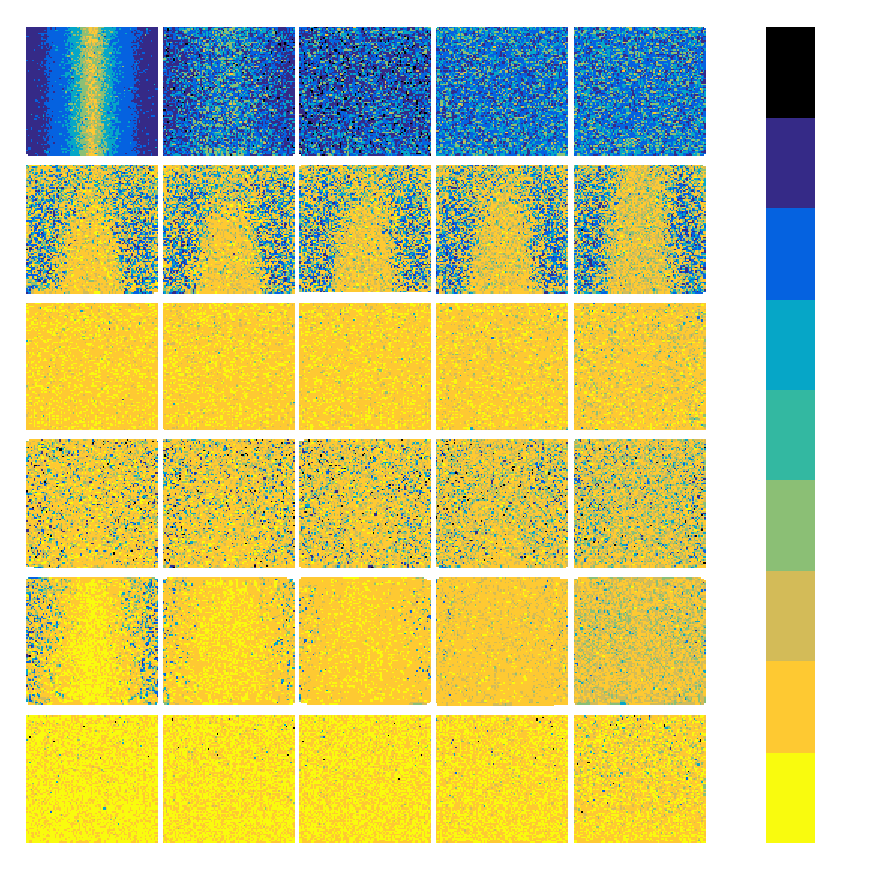
\includegraphics{./figures/parts/appendix/chapters/05/sections/04/caer_style_orientation_errors_binned_dxyt4}}%
    \gplfronttext
  \end{picture}%
\endgroup

  \vspace{1cm}
  \caption{\small Χάρτες θερμότητας των μέτρων των τελικών σφαλμάτων εκτίμησης
           προσανατολισμού συναρτήσει των αρχικών σφαλμάτων εκτίμησης
           προσανατολισμού $\Delta\hat{\theta} \in
           [-\overline{\delta}_{\theta},+\overline{\delta}_{\theta}]$ (στον
           οριζόντιο άξονα) και των μέτρων των αρχικών σφαλμάτων εκτίμησης
           θέσης $\|\Delta \hat{\bm{l}}\|_2 \in [0, \sqrt{2}\cdot
           \overline{\delta}_{xy}]$ (στον κάθετο άξονα) για όλα τα
           διενεργηθέντα πειράματα, ανά αλγόριθμο και ανά τυπική απόκλιση
           διαταραχών του φυσικού αισθητήρα, για τη διάταξη με
           $(\overline{\delta}_{xy}, \overline{\delta}_{\theta}) = (0.20,
           0.30)$ [m,rad]}
  \label{fig:appendix_05_01:10}
\end{figure}
\begin{figure}\vspace{1cm}\hspace{0.5cm}
  % GNUPLOT: LaTeX picture with Postscript
\begingroup
  \makeatletter
  \providecommand\color[2][]{%
    \GenericError{(gnuplot) \space\space\space\@spaces}{%
      Package color not loaded in conjunction with
      terminal option `colourtext'%
    }{See the gnuplot documentation for explanation.%
    }{Either use 'blacktext' in gnuplot or load the package
      color.sty in LaTeX.}%
    \renewcommand\color[2][]{}%
  }%
  \providecommand\includegraphics[2][]{%
    \GenericError{(gnuplot) \space\space\space\@spaces}{%
      Package graphicx or graphics not loaded%
    }{See the gnuplot documentation for explanation.%
    }{The gnuplot epslatex terminal needs graphicx.sty or graphics.sty.}%
    \renewcommand\includegraphics[2][]{}%
  }%
  \providecommand\rotatebox[2]{#2}%
  \@ifundefined{ifGPcolor}{%
    \newif\ifGPcolor
    \GPcolorfalse
  }{}%
  \@ifundefined{ifGPblacktext}{%
    \newif\ifGPblacktext
    \GPblacktexttrue
  }{}%
  % define a \g@addto@macro without @ in the name:
  \let\gplgaddtomacro\g@addto@macro
  % define empty templates for all commands taking text:
  \gdef\gplbacktext{}%
  \gdef\gplfronttext{}%
  \makeatother
  \ifGPblacktext
    % no textcolor at all
    \def\colorrgb#1{}%
    \def\colorgray#1{}%
  \else
    % gray or color?
    \ifGPcolor
      \def\colorrgb#1{\color[rgb]{#1}}%
      \def\colorgray#1{\color[gray]{#1}}%
      \expandafter\def\csname LTw\endcsname{\color{white}}%
      \expandafter\def\csname LTb\endcsname{\color{black}}%
      \expandafter\def\csname LTa\endcsname{\color{black}}%
      \expandafter\def\csname LT0\endcsname{\color[rgb]{1,0,0}}%
      \expandafter\def\csname LT1\endcsname{\color[rgb]{0,1,0}}%
      \expandafter\def\csname LT2\endcsname{\color[rgb]{0,0,1}}%
      \expandafter\def\csname LT3\endcsname{\color[rgb]{1,0,1}}%
      \expandafter\def\csname LT4\endcsname{\color[rgb]{0,1,1}}%
      \expandafter\def\csname LT5\endcsname{\color[rgb]{1,1,0}}%
      \expandafter\def\csname LT6\endcsname{\color[rgb]{0,0,0}}%
      \expandafter\def\csname LT7\endcsname{\color[rgb]{1,0.3,0}}%
      \expandafter\def\csname LT8\endcsname{\color[rgb]{0.5,0.5,0.5}}%
    \else
      % gray
      \def\colorrgb#1{\color{black}}%
      \def\colorgray#1{\color[gray]{#1}}%
      \expandafter\def\csname LTw\endcsname{\color{white}}%
      \expandafter\def\csname LTb\endcsname{\color{black}}%
      \expandafter\def\csname LTa\endcsname{\color{black}}%
      \expandafter\def\csname LT0\endcsname{\color{black}}%
      \expandafter\def\csname LT1\endcsname{\color{black}}%
      \expandafter\def\csname LT2\endcsname{\color{black}}%
      \expandafter\def\csname LT3\endcsname{\color{black}}%
      \expandafter\def\csname LT4\endcsname{\color{black}}%
      \expandafter\def\csname LT5\endcsname{\color{black}}%
      \expandafter\def\csname LT6\endcsname{\color{black}}%
      \expandafter\def\csname LT7\endcsname{\color{black}}%
      \expandafter\def\csname LT8\endcsname{\color{black}}%
    \fi
  \fi
  \setlength{\unitlength}{0.0500bp}%
  \begin{picture}(8000.00,8000.00)%
     \gplgaddtomacro\gplfronttext{%
      \colorrgb{0.00,0.00,0.00}%
      \put(716,8200){\makebox(0,0){\strut{}\small $\sigma_R = 0.01$}}%
      \colorrgb{0.00,0.00,0.00}%
      \put(2029,8200){\makebox(0,0){\strut{}\small $\sigma_R = 0.03$}}%
      \colorrgb{0.00,0.00,0.00}%
      \put(3343,8200){\makebox(0,0){\strut{}\small $\sigma_R = 0.05$}}%
      \colorrgb{0.00,0.00,0.00}%
      \put(4656,8200){\makebox(0,0){\strut{}\small $\sigma_R = 0.10$}}%
      \colorrgb{0.00,0.00,0.00}%
      \put(5969,8200){\makebox(0,0){\strut{}\small $\sigma_R = 0.20$ [m]}}%
      \put(3333.33,8700){\makebox(0,0){\strut{}$(\overline{\delta}_{xy}, \overline{\delta}_\theta) = (0.20 \ \text{m}, 0.56 \ \text{rad})$}}
      \put(4000,9200){\makebox(0,0){\strut{}Τελικά σφάλματα εκτίμησης προσανατολισμού ως προς αρχικές συνθήκες μετατόπισης [rad]}}
    }%
    \gplgaddtomacro\gplfronttext{%
      \colorrgb{0.00,0.00,0.00}%
      \put(-200,7333.33){\rotatebox{90}{\makebox(0,0){\strut{}\small PLICP}}}%
    }%
    \gplgaddtomacro\gplfronttext{%
      \colorrgb{0.00,0.00,0.00}%
      \put(-200,6000){\rotatebox{90}{\makebox(0,0){\strut{}\small NDT}}}%
    }%
    \gplgaddtomacro\gplfronttext{%
      \colorrgb{0.00,0.00,0.00}%
      \put(-200,4666.66){\rotatebox{90}{\makebox(0,0){\strut{}\small FastGICP}}}%
    }%
    \gplgaddtomacro\gplfronttext{%
      \colorrgb{0.00,0.00,0.00}%
      \put(-200,3333.33){\rotatebox{90}{\makebox(0,0){\strut{}\small FastVGICP}}}%
    }%
    \gplgaddtomacro\gplfronttext{%
      \colorrgb{0.00,0.00,0.00}%
      \put(-200,2000){\rotatebox{90}{\makebox(0,0){\strut{}\small NDT-PSO}}}%
    }%
    \gplgaddtomacro\gplfronttext{%
      \colorrgb{0.00,0.00,0.00}%
      \put(-200,666.66){\rotatebox{90}{\makebox(0,0){\strut{}\small \texttt{fsm}}}}%
    }%
    \gplgaddtomacro\gplfronttext{%
      \colorrgb{0.00,0.00,0.00}%
      \put(7800,515.5){\makebox(0,0)[l]{\strut{}$<0.001$}}%
      \colorrgb{0.00,0.00,0.00}%
      \put(7800,1386.5){\makebox(0,0)[l]{\strut{}$<0.01$}}%
      \colorrgb{0.00,0.00,0.00}%
      \put(7800,2257.5){\makebox(0,0)[l]{\strut{}$<0.02$}}%
      \colorrgb{0.00,0.00,0.00}%
      \put(7800,3128.5){\makebox(0,0)[l]{\strut{}$<0.05$}}%
      \colorrgb{0.00,0.00,0.00}%
      \put(7800,3999.5){\makebox(0,0)[l]{\strut{}$<0.1$}}%
      \colorrgb{0.00,0.00,0.00}%
      \put(7800,4870.5){\makebox(0,0)[l]{\strut{}$<0.2$}}%
      \colorrgb{0.00,0.00,0.00}%
      \put(7800,5741.5){\makebox(0,0)[l]{\strut{}$<0.5$}}%
      \colorrgb{0.00,0.00,0.00}%
      \put(7800,6612.5){\makebox(0,0)[l]{\strut{}$<1$}}%
      \colorrgb{0.00,0.00,0.00}%
      \put(7800,7483.5){\makebox(0,0)[l]{\strut{}$<e^{\overline{\delta}_{xy}, \overline{\delta}_\theta}_{\theta,\max} = 3.062$}}%
    }%
    \put(0,0){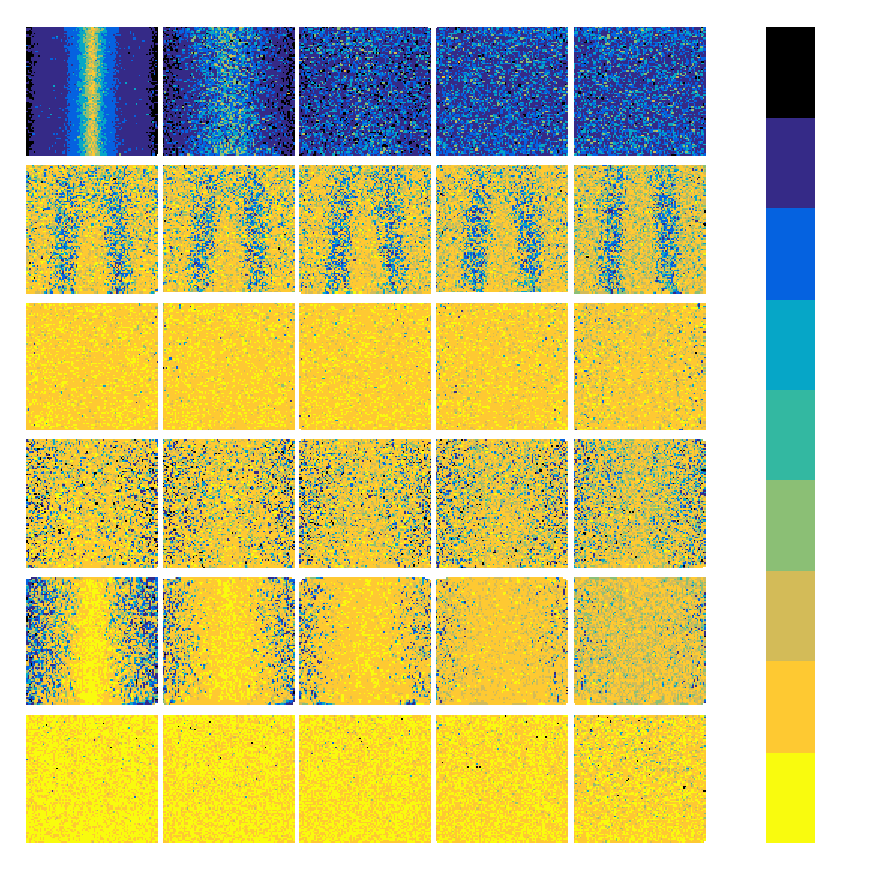
\includegraphics{./figures/parts/appendix/chapters/05/sections/04/caer_style_orientation_errors_binned_dxyt5}}%
    \gplfronttext
  \end{picture}%
\endgroup

  \vspace{1cm}
  \caption{\small Χάρτες θερμότητας των μέτρων των τελικών σφαλμάτων εκτίμησης
           προσανατολισμού συναρτήσει των αρχικών σφαλμάτων εκτίμησης
           προσανατολισμού $\Delta\hat{\theta} \in
           [-\overline{\delta}_{\theta},+\overline{\delta}_{\theta}]$ (στον
           οριζόντιο άξονα) και των μέτρων των αρχικών σφαλμάτων εκτίμησης
           θέσης $\|\Delta \hat{\bm{l}}\|_2 \in [0, \sqrt{2}\cdot
           \overline{\delta}_{xy}]$ (στον κάθετο άξονα) για όλα τα
           διενεργηθέντα πειράματα, ανά αλγόριθμο και ανά τυπική απόκλιση
           διαταραχών του φυσικού αισθητήρα, για τη διάταξη με
           $(\overline{\delta}_{xy}, \overline{\delta}_{\theta}) = (0.20,
           0.56)$ [m,rad]}
  \label{fig:appendix_05_01:11}
\end{figure}
\begin{figure}\vspace{1cm}\hspace{0.5cm}
  % GNUPLOT: LaTeX picture with Postscript
\begingroup
  \makeatletter
  \providecommand\color[2][]{%
    \GenericError{(gnuplot) \space\space\space\@spaces}{%
      Package color not loaded in conjunction with
      terminal option `colourtext'%
    }{See the gnuplot documentation for explanation.%
    }{Either use 'blacktext' in gnuplot or load the package
      color.sty in LaTeX.}%
    \renewcommand\color[2][]{}%
  }%
  \providecommand\includegraphics[2][]{%
    \GenericError{(gnuplot) \space\space\space\@spaces}{%
      Package graphicx or graphics not loaded%
    }{See the gnuplot documentation for explanation.%
    }{The gnuplot epslatex terminal needs graphicx.sty or graphics.sty.}%
    \renewcommand\includegraphics[2][]{}%
  }%
  \providecommand\rotatebox[2]{#2}%
  \@ifundefined{ifGPcolor}{%
    \newif\ifGPcolor
    \GPcolorfalse
  }{}%
  \@ifundefined{ifGPblacktext}{%
    \newif\ifGPblacktext
    \GPblacktexttrue
  }{}%
  % define a \g@addto@macro without @ in the name:
  \let\gplgaddtomacro\g@addto@macro
  % define empty templates for all commands taking text:
  \gdef\gplbacktext{}%
  \gdef\gplfronttext{}%
  \makeatother
  \ifGPblacktext
    % no textcolor at all
    \def\colorrgb#1{}%
    \def\colorgray#1{}%
  \else
    % gray or color?
    \ifGPcolor
      \def\colorrgb#1{\color[rgb]{#1}}%
      \def\colorgray#1{\color[gray]{#1}}%
      \expandafter\def\csname LTw\endcsname{\color{white}}%
      \expandafter\def\csname LTb\endcsname{\color{black}}%
      \expandafter\def\csname LTa\endcsname{\color{black}}%
      \expandafter\def\csname LT0\endcsname{\color[rgb]{1,0,0}}%
      \expandafter\def\csname LT1\endcsname{\color[rgb]{0,1,0}}%
      \expandafter\def\csname LT2\endcsname{\color[rgb]{0,0,1}}%
      \expandafter\def\csname LT3\endcsname{\color[rgb]{1,0,1}}%
      \expandafter\def\csname LT4\endcsname{\color[rgb]{0,1,1}}%
      \expandafter\def\csname LT5\endcsname{\color[rgb]{1,1,0}}%
      \expandafter\def\csname LT6\endcsname{\color[rgb]{0,0,0}}%
      \expandafter\def\csname LT7\endcsname{\color[rgb]{1,0.3,0}}%
      \expandafter\def\csname LT8\endcsname{\color[rgb]{0.5,0.5,0.5}}%
    \else
      % gray
      \def\colorrgb#1{\color{black}}%
      \def\colorgray#1{\color[gray]{#1}}%
      \expandafter\def\csname LTw\endcsname{\color{white}}%
      \expandafter\def\csname LTb\endcsname{\color{black}}%
      \expandafter\def\csname LTa\endcsname{\color{black}}%
      \expandafter\def\csname LT0\endcsname{\color{black}}%
      \expandafter\def\csname LT1\endcsname{\color{black}}%
      \expandafter\def\csname LT2\endcsname{\color{black}}%
      \expandafter\def\csname LT3\endcsname{\color{black}}%
      \expandafter\def\csname LT4\endcsname{\color{black}}%
      \expandafter\def\csname LT5\endcsname{\color{black}}%
      \expandafter\def\csname LT6\endcsname{\color{black}}%
      \expandafter\def\csname LT7\endcsname{\color{black}}%
      \expandafter\def\csname LT8\endcsname{\color{black}}%
    \fi
  \fi
  \setlength{\unitlength}{0.0500bp}%
  \begin{picture}(8000.00,8000.00)%
     \gplgaddtomacro\gplfronttext{%
      \colorrgb{0.00,0.00,0.00}%
      \put(716,8200){\makebox(0,0){\strut{}\small $\sigma_R = 0.01$}}%
      \colorrgb{0.00,0.00,0.00}%
      \put(2029,8200){\makebox(0,0){\strut{}\small $\sigma_R = 0.03$}}%
      \colorrgb{0.00,0.00,0.00}%
      \put(3343,8200){\makebox(0,0){\strut{}\small $\sigma_R = 0.05$}}%
      \colorrgb{0.00,0.00,0.00}%
      \put(4656,8200){\makebox(0,0){\strut{}\small $\sigma_R = 0.10$}}%
      \colorrgb{0.00,0.00,0.00}%
      \put(5969,8200){\makebox(0,0){\strut{}\small $\sigma_R = 0.20$ [m]}}%
    }%
    \gplgaddtomacro\gplfronttext{%
      \colorrgb{0.00,0.00,0.00}%
      \put(-200,7333.33){\rotatebox{90}{\makebox(0,0){\strut{}\small PLICP}}}%
    }%
    \gplgaddtomacro\gplfronttext{%
      \colorrgb{0.00,0.00,0.00}%
      \put(-200,6000){\rotatebox{90}{\makebox(0,0){\strut{}\small NDT}}}%
    }%
    \gplgaddtomacro\gplfronttext{%
      \colorrgb{0.00,0.00,0.00}%
      \put(-200,4666.66){\rotatebox{90}{\makebox(0,0){\strut{}\small FastGICP}}}%
    }%
    \gplgaddtomacro\gplfronttext{%
      \colorrgb{0.00,0.00,0.00}%
      \put(-200,3333.33){\rotatebox{90}{\makebox(0,0){\strut{}\small FastVGICP}}}%
    }%
    \gplgaddtomacro\gplfronttext{%
      \colorrgb{0.00,0.00,0.00}%
      \put(-200,2000){\rotatebox{90}{\makebox(0,0){\strut{}\small NDT-PSO}}}%
    }%
    \gplgaddtomacro\gplfronttext{%
      \colorrgb{0.00,0.00,0.00}%
      \put(-200,666.66){\rotatebox{90}{\makebox(0,0){\strut{}\small \texttt{fsm}}}}%
    }%
    \gplgaddtomacro\gplfronttext{%
      \colorrgb{0.00,0.00,0.00}%
      \put(7800,515.5){\makebox(0,0)[l]{\strut{}$<0.001$}}%
      \colorrgb{0.00,0.00,0.00}%
      \put(7800,1386.5){\makebox(0,0)[l]{\strut{}$<0.01$}}%
      \colorrgb{0.00,0.00,0.00}%
      \put(7800,2257.5){\makebox(0,0)[l]{\strut{}$<0.02$}}%
      \colorrgb{0.00,0.00,0.00}%
      \put(7800,3128.5){\makebox(0,0)[l]{\strut{}$<0.05$}}%
      \colorrgb{0.00,0.00,0.00}%
      \put(7800,3999.5){\makebox(0,0)[l]{\strut{}$<0.1$}}%
      \colorrgb{0.00,0.00,0.00}%
      \put(7800,4870.5){\makebox(0,0)[l]{\strut{}$<0.2$}}%
      \colorrgb{0.00,0.00,0.00}%
      \put(7800,5741.5){\makebox(0,0)[l]{\strut{}$<0.5$}}%
      \colorrgb{0.00,0.00,0.00}%
      \put(7800,6612.5){\makebox(0,0)[l]{\strut{}$<1$}}%
      \colorrgb{0.00,0.00,0.00}%
      \put(7800,7483.5){\makebox(0,0)[l]{\strut{}$<3.0181$}}%
    }%

    \put(0,0){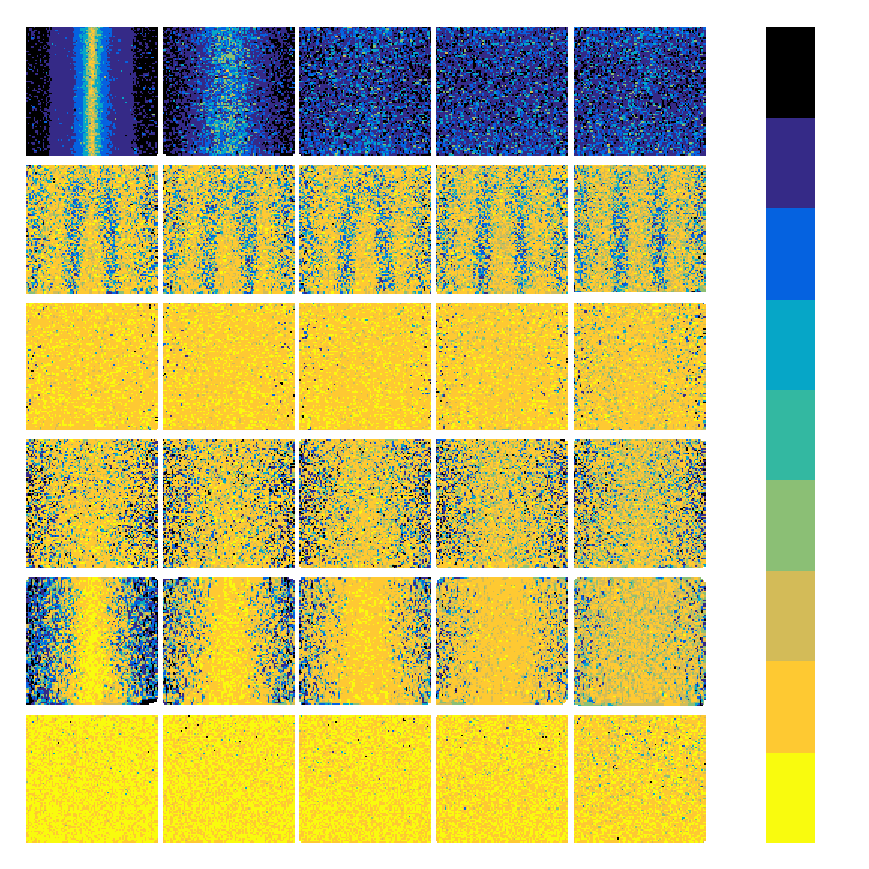
\includegraphics{./figures/parts/02/chapters/05/sections/04/caer_style_orientation_errors_binned_dxyt6}}%
    \gplfronttext
  \end{picture}%
\endgroup

  \vspace{1cm}
  \caption{\small Χάρτες θερμότητας των μέτρων των τελικών σφαλμάτων εκτίμησης
           προσανατολισμού συναρτήσει των αρχικών σφαλμάτων εκτίμησης
           προσανατολισμού $\Delta\hat{\theta} \in
           [-\overline{\delta}_{\theta},+\overline{\delta}_{\theta}]$ (στον
           οριζόντιο άξονα) και των μέτρων των αρχικών σφαλμάτων εκτίμησης
           θέσης $\|\Delta \hat{\bm{l}}\|_2 \in [0, \sqrt{2}\cdot
           \overline{\delta}_{xy}]$ (στον κάθετο άξονα) για όλα τα
           διενεργηθέντα πειράματα, ανά αλγόριθμο και ανά τυπική απόκλιση
           διαταραχών του φυσικού αισθητήρα, για τη διάταξη με
           $(\overline{\delta}_{xy}, \overline{\delta}_{\theta}) = (0.20,
           \pi/4)$ [m,rad]}
  \label{fig:appendix_05_01:12}
\end{figure}


























\begin{figure}\vspace{1cm}\hspace{0.5cm}
  % GNUPLOT: LaTeX picture with Postscript
\begingroup
  \makeatletter
  \providecommand\color[2][]{%
    \GenericError{(gnuplot) \space\space\space\@spaces}{%
      Package color not loaded in conjunction with
      terminal option `colourtext'%
    }{See the gnuplot documentation for explanation.%
    }{Either use 'blacktext' in gnuplot or load the package
      color.sty in LaTeX.}%
    \renewcommand\color[2][]{}%
  }%
  \providecommand\includegraphics[2][]{%
    \GenericError{(gnuplot) \space\space\space\@spaces}{%
      Package graphicx or graphics not loaded%
    }{See the gnuplot documentation for explanation.%
    }{The gnuplot epslatex terminal needs graphicx.sty or graphics.sty.}%
    \renewcommand\includegraphics[2][]{}%
  }%
  \providecommand\rotatebox[2]{#2}%
  \@ifundefined{ifGPcolor}{%
    \newif\ifGPcolor
    \GPcolorfalse
  }{}%
  \@ifundefined{ifGPblacktext}{%
    \newif\ifGPblacktext
    \GPblacktexttrue
  }{}%
  % define a \g@addto@macro without @ in the name:
  \let\gplgaddtomacro\g@addto@macro
  % define empty templates for all commands taking text:
  \gdef\gplfronttext{}%
  \gdef\gplfronttext{}%
  \makeatother
  \ifGPblacktext
    % no textcolor at all
    \def\colorrgb#1{}%
    \def\colorgray#1{}%
  \else
    % gray or color?
    \ifGPcolor
      \def\colorrgb#1{\color[rgb]{#1}}%
      \def\colorgray#1{\color[gray]{#1}}%
      \expandafter\def\csname LTw\endcsname{\color{white}}%
      \expandafter\def\csname LTb\endcsname{\color{black}}%
      \expandafter\def\csname LTa\endcsname{\color{black}}%
      \expandafter\def\csname LT0\endcsname{\color[rgb]{1,0,0}}%
      \expandafter\def\csname LT1\endcsname{\color[rgb]{0,1,0}}%
      \expandafter\def\csname LT2\endcsname{\color[rgb]{0,0,1}}%
      \expandafter\def\csname LT3\endcsname{\color[rgb]{1,0,1}}%
      \expandafter\def\csname LT4\endcsname{\color[rgb]{0,1,1}}%
      \expandafter\def\csname LT5\endcsname{\color[rgb]{1,1,0}}%
      \expandafter\def\csname LT6\endcsname{\color[rgb]{0,0,0}}%
      \expandafter\def\csname LT7\endcsname{\color[rgb]{1,0.3,0}}%
      \expandafter\def\csname LT8\endcsname{\color[rgb]{0.5,0.5,0.5}}%
    \else
      % gray
      \def\colorrgb#1{\color{black}}%
      \def\colorgray#1{\color[gray]{#1}}%
      \expandafter\def\csname LTw\endcsname{\color{white}}%
      \expandafter\def\csname LTb\endcsname{\color{black}}%
      \expandafter\def\csname LTa\endcsname{\color{black}}%
      \expandafter\def\csname LT0\endcsname{\color{black}}%
      \expandafter\def\csname LT1\endcsname{\color{black}}%
      \expandafter\def\csname LT2\endcsname{\color{black}}%
      \expandafter\def\csname LT3\endcsname{\color{black}}%
      \expandafter\def\csname LT4\endcsname{\color{black}}%
      \expandafter\def\csname LT5\endcsname{\color{black}}%
      \expandafter\def\csname LT6\endcsname{\color{black}}%
      \expandafter\def\csname LT7\endcsname{\color{black}}%
      \expandafter\def\csname LT8\endcsname{\color{black}}%
    \fi
  \fi
  \setlength{\unitlength}{0.0500bp}%
  \begin{picture}(8000.00,8000.00)%
     \gplgaddtomacro\gplfronttext{%
      \colorrgb{0.00,0.00,0.00}%
      \put(716,8200){\makebox(0,0){\strut{}\small $\sigma_R = 0.01$}}%
      \colorrgb{0.00,0.00,0.00}%
      \put(2029,8200){\makebox(0,0){\strut{}\small $\sigma_R = 0.03$}}%
      \colorrgb{0.00,0.00,0.00}%
      \put(3343,8200){\makebox(0,0){\strut{}\small $\sigma_R = 0.05$}}%
      \colorrgb{0.00,0.00,0.00}%
      \put(4656,8200){\makebox(0,0){\strut{}\small $\sigma_R = 0.10$}}%
      \colorrgb{0.00,0.00,0.00}%
      \put(5969,8200){\makebox(0,0){\strut{}\small $\sigma_R = 0.20$ [m]}}%
    }%
    \gplgaddtomacro\gplfronttext{%
      \colorrgb{0.00,0.00,0.00}%
      \put(-200,7333.33){\rotatebox{90}{\makebox(0,0){\strut{}\small PLICP}}}%
    }%
    \gplgaddtomacro\gplfronttext{%
      \colorrgb{0.00,0.00,0.00}%
      \put(-200,6000){\rotatebox{90}{\makebox(0,0){\strut{}\small NDT}}}%
    }%
    \gplgaddtomacro\gplfronttext{%
      \colorrgb{0.00,0.00,0.00}%
      \put(-200,4666.66){\rotatebox{90}{\makebox(0,0){\strut{}\small FastGICP}}}%
    }%
    \gplgaddtomacro\gplfronttext{%
      \colorrgb{0.00,0.00,0.00}%
      \put(-200,3333.33){\rotatebox{90}{\makebox(0,0){\strut{}\small FastVGICP}}}%
    }%
    \gplgaddtomacro\gplfronttext{%
      \colorrgb{0.00,0.00,0.00}%
      \put(-200,2000){\rotatebox{90}{\makebox(0,0){\strut{}\small NDT-PSO}}}%
    }%
    \gplgaddtomacro\gplfronttext{%
      \colorrgb{0.00,0.00,0.00}%
      \put(-200,666.66){\rotatebox{90}{\makebox(0,0){\strut{}\small \texttt{fsm}}}}%
    }%

    \gplgaddtomacro\gplfronttext{%
      \colorrgb{0.00,0.00,0.00}%
      \put(7800,80){\makebox(0,0)[l]{\strut{}$0.0$}}%
      \colorrgb{0.00,0.00,0.00}%
      \put(7800,1399){\makebox(0,0)[l]{\strut{}$0.01$}}%
      \colorrgb{0.00,0.00,0.00}%
      \put(7800,2718){\makebox(0,0)[l]{\strut{}$0.02$}}%
      \colorrgb{0.00,0.00,0.00}%
      \put(7800,4037){\makebox(0,0)[l]{\strut{}$0.03$}}%
      \colorrgb{0.00,0.00,0.00}%
      \put(7800,5356){\makebox(0,0)[l]{\strut{}$0.04$}}%
      \colorrgb{0.00,0.00,0.00}%
      \put(7800,6675){\makebox(0,0)[l]{\strut{}$0.05$}}%
      \colorrgb{0.00,0.00,0.00}%
      \put(7800,7919){\makebox(0,0)[l]{\strut{}$> 0.059431$}}%
    }%
    \put(0,0){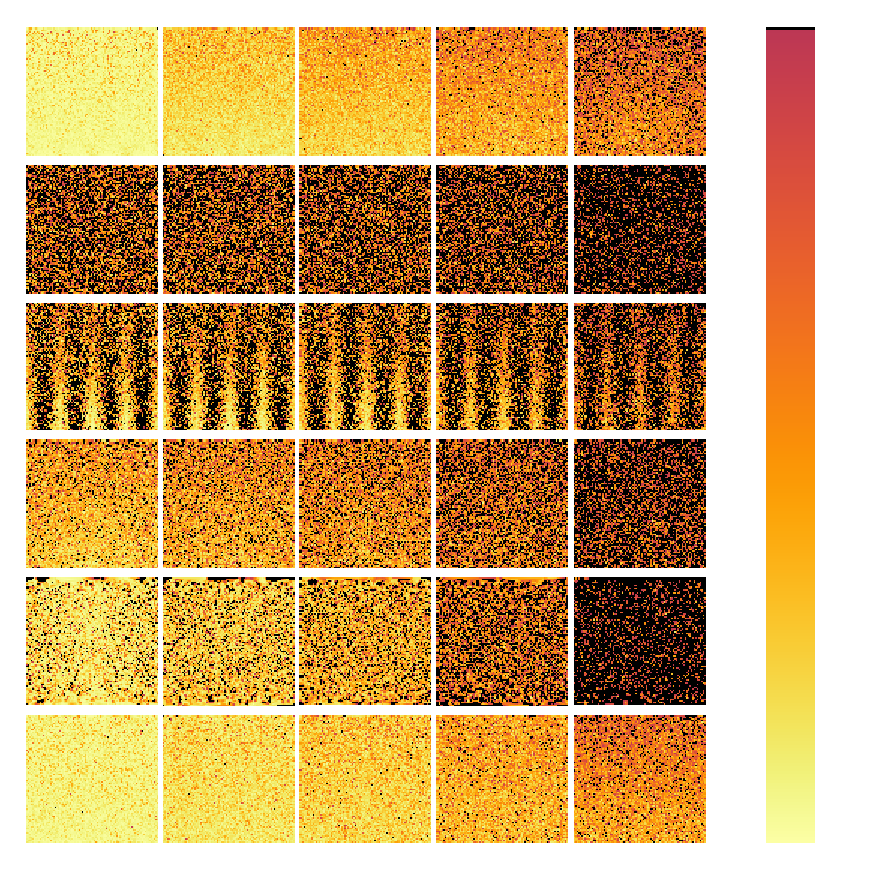
\includegraphics{./figures/parts/appendix/chapters/05/sections/04/caer_style_position_errors_dxyt1}}%
    \gplfronttext
  \end{picture}%
\endgroup

  \vspace{1cm}
  \caption{\small Χάρτες θερμότητας των μέτρων των τελικών σφαλμάτων εκτίμησης
           θέσης συναρτήσει των αρχικών σφαλμάτων εκτίμησης προσανατολισμού
           $\Delta\hat{\theta} \in
           [-\overline{\delta}_{\theta},+\overline{\delta}_{\theta}]$ (στον
           οριζόντιο άξονα) και των μέτρων των αρχικών σφαλμάτων εκτίμησης
           θέσης $\|\Delta \hat{\bm{l}}\|_2 \in [0, \sqrt{2}\cdot
           \overline{\delta}_{xy}]$ (στον κάθετο άξονα) για όλα τα
           διενεργηθέντα πειράματα, ανά αλγόριθμο και ανά τυπική απόκλιση
           διαταραχών του φυσικού αισθητήρα, για τη διάταξη με
           $(\overline{\delta}_{xy}, \overline{\delta}_{\theta}) = (0.05,
           0.035)$ [m,rad], εστιασμένοι στο διάστημα $[0,
           e_{xy,\text{avg}}^{\overline{\delta}_{xy},
           \overline{\delta}_{\theta}}]$, όπου με
           $e_{xy,\text{avg}}^{\overline{\delta}_{xy},
           \overline{\delta}_{\theta}}$ σημειώνεται ο μέσος όρος σφάλματος
           εκτίμησης στάσης όλων των μεθόδων, για κάθε επεξεργασθέν δείγμα, και
           κάθε τιμή τυπικής απόκλισης των διαταραχών που επιδρούν στις
           μετρήσεις του φυσικού αισθητήρα, για τη διαμόρφωση
           $(\overline{\delta}_{xy}, \overline{\delta}_{\theta})$.  Τιμές
           μέτρου σφάλματος εκτίμησης άνω του μέσου όρου σημειώνονται με μαύρο
           χρώμα}
  \label{fig:appendix_05_01:13}
\end{figure}
\begin{figure}\vspace{1cm}\hspace{0.5cm}
  % GNUPLOT: LaTeX picture with Postscript
\begingroup
  \makeatletter
  \providecommand\color[2][]{%
    \GenericError{(gnuplot) \space\space\space\@spaces}{%
      Package color not loaded in conjunction with
      terminal option `colourtext'%
    }{See the gnuplot documentation for explanation.%
    }{Either use 'blacktext' in gnuplot or load the package
      color.sty in LaTeX.}%
    \renewcommand\color[2][]{}%
  }%
  \providecommand\includegraphics[2][]{%
    \GenericError{(gnuplot) \space\space\space\@spaces}{%
      Package graphicx or graphics not loaded%
    }{See the gnuplot documentation for explanation.%
    }{The gnuplot epslatex terminal needs graphicx.sty or graphics.sty.}%
    \renewcommand\includegraphics[2][]{}%
  }%
  \providecommand\rotatebox[2]{#2}%
  \@ifundefined{ifGPcolor}{%
    \newif\ifGPcolor
    \GPcolorfalse
  }{}%
  \@ifundefined{ifGPblacktext}{%
    \newif\ifGPblacktext
    \GPblacktexttrue
  }{}%
  % define a \g@addto@macro without @ in the name:
  \let\gplgaddtomacro\g@addto@macro
  % define empty templates for all commands taking text:
  \gdef\gplfronttext{}%
  \gdef\gplfronttext{}%
  \makeatother
  \ifGPblacktext
    % no textcolor at all
    \def\colorrgb#1{}%
    \def\colorgray#1{}%
  \else
    % gray or color?
    \ifGPcolor
      \def\colorrgb#1{\color[rgb]{#1}}%
      \def\colorgray#1{\color[gray]{#1}}%
      \expandafter\def\csname LTw\endcsname{\color{white}}%
      \expandafter\def\csname LTb\endcsname{\color{black}}%
      \expandafter\def\csname LTa\endcsname{\color{black}}%
      \expandafter\def\csname LT0\endcsname{\color[rgb]{1,0,0}}%
      \expandafter\def\csname LT1\endcsname{\color[rgb]{0,1,0}}%
      \expandafter\def\csname LT2\endcsname{\color[rgb]{0,0,1}}%
      \expandafter\def\csname LT3\endcsname{\color[rgb]{1,0,1}}%
      \expandafter\def\csname LT4\endcsname{\color[rgb]{0,1,1}}%
      \expandafter\def\csname LT5\endcsname{\color[rgb]{1,1,0}}%
      \expandafter\def\csname LT6\endcsname{\color[rgb]{0,0,0}}%
      \expandafter\def\csname LT7\endcsname{\color[rgb]{1,0.3,0}}%
      \expandafter\def\csname LT8\endcsname{\color[rgb]{0.5,0.5,0.5}}%
    \else
      % gray
      \def\colorrgb#1{\color{black}}%
      \def\colorgray#1{\color[gray]{#1}}%
      \expandafter\def\csname LTw\endcsname{\color{white}}%
      \expandafter\def\csname LTb\endcsname{\color{black}}%
      \expandafter\def\csname LTa\endcsname{\color{black}}%
      \expandafter\def\csname LT0\endcsname{\color{black}}%
      \expandafter\def\csname LT1\endcsname{\color{black}}%
      \expandafter\def\csname LT2\endcsname{\color{black}}%
      \expandafter\def\csname LT3\endcsname{\color{black}}%
      \expandafter\def\csname LT4\endcsname{\color{black}}%
      \expandafter\def\csname LT5\endcsname{\color{black}}%
      \expandafter\def\csname LT6\endcsname{\color{black}}%
      \expandafter\def\csname LT7\endcsname{\color{black}}%
      \expandafter\def\csname LT8\endcsname{\color{black}}%
    \fi
  \fi
  \setlength{\unitlength}{0.0500bp}%
  \begin{picture}(8000.00,8000.00)%
     \gplgaddtomacro\gplfronttext{%
      \colorrgb{0.00,0.00,0.00}%
      \put(716,8200){\makebox(0,0){\strut{}\small $\sigma_R = 0.01$}}%
      \colorrgb{0.00,0.00,0.00}%
      \put(2029,8200){\makebox(0,0){\strut{}\small $\sigma_R = 0.03$}}%
      \colorrgb{0.00,0.00,0.00}%
      \put(3343,8200){\makebox(0,0){\strut{}\small $\sigma_R = 0.05$}}%
      \colorrgb{0.00,0.00,0.00}%
      \put(4656,8200){\makebox(0,0){\strut{}\small $\sigma_R = 0.10$}}%
      \colorrgb{0.00,0.00,0.00}%
      \put(5969,8200){\makebox(0,0){\strut{}\small $\sigma_R = 0.20$ [m]}}%
    }%
    \gplgaddtomacro\gplfronttext{%
      \colorrgb{0.00,0.00,0.00}%
      \put(-200,7333.33){\rotatebox{90}{\makebox(0,0){\strut{}\small PLICP}}}%
    }%
    \gplgaddtomacro\gplfronttext{%
      \colorrgb{0.00,0.00,0.00}%
      \put(-200,6000){\rotatebox{90}{\makebox(0,0){\strut{}\small NDT}}}%
    }%
    \gplgaddtomacro\gplfronttext{%
      \colorrgb{0.00,0.00,0.00}%
      \put(-200,4666.66){\rotatebox{90}{\makebox(0,0){\strut{}\small FastGICP}}}%
    }%
    \gplgaddtomacro\gplfronttext{%
      \colorrgb{0.00,0.00,0.00}%
      \put(-200,3333.33){\rotatebox{90}{\makebox(0,0){\strut{}\small FastVGICP}}}%
    }%
    \gplgaddtomacro\gplfronttext{%
      \colorrgb{0.00,0.00,0.00}%
      \put(-200,2000){\rotatebox{90}{\makebox(0,0){\strut{}\small NDT-PSO}}}%
    }%
    \gplgaddtomacro\gplfronttext{%
      \colorrgb{0.00,0.00,0.00}%
      \put(-200,666.66){\rotatebox{90}{\makebox(0,0){\strut{}\small \texttt{fsm}}}}%
    }%
    \gplgaddtomacro\gplfronttext{%
      \colorrgb{0.00,0.00,0.00}%
      \put(7800,80){\makebox(0,0)[l]{\strut{}$0.0$}}%
      \colorrgb{0.00,0.00,0.00}%
      \put(7800,1267){\makebox(0,0)[l]{\strut{}$0.01$}}%
      \colorrgb{0.00,0.00,0.00}%
      \put(7800,2453){\makebox(0,0)[l]{\strut{}$0.02$}}%
      \colorrgb{0.00,0.00,0.00}%
      \put(7800,3640){\makebox(0,0)[l]{\strut{}$0.03$}}%
      \colorrgb{0.00,0.00,0.00}%
      \put(7800,4827){\makebox(0,0)[l]{\strut{}$0.04$}}%
      \colorrgb{0.00,0.00,0.00}%
      \put(7800,6014){\makebox(0,0)[l]{\strut{}$0.05$}}%
      \colorrgb{0.00,0.00,0.00}%
      \put(7800,7200){\makebox(0,0)[l]{\strut{}$0.06$}}%
      \colorrgb{0.00,0.00,0.00}%
      \put(7800,7919){\makebox(0,0)[l]{\strut{}$> 0.066057$}}%
    }%
    \put(0,0){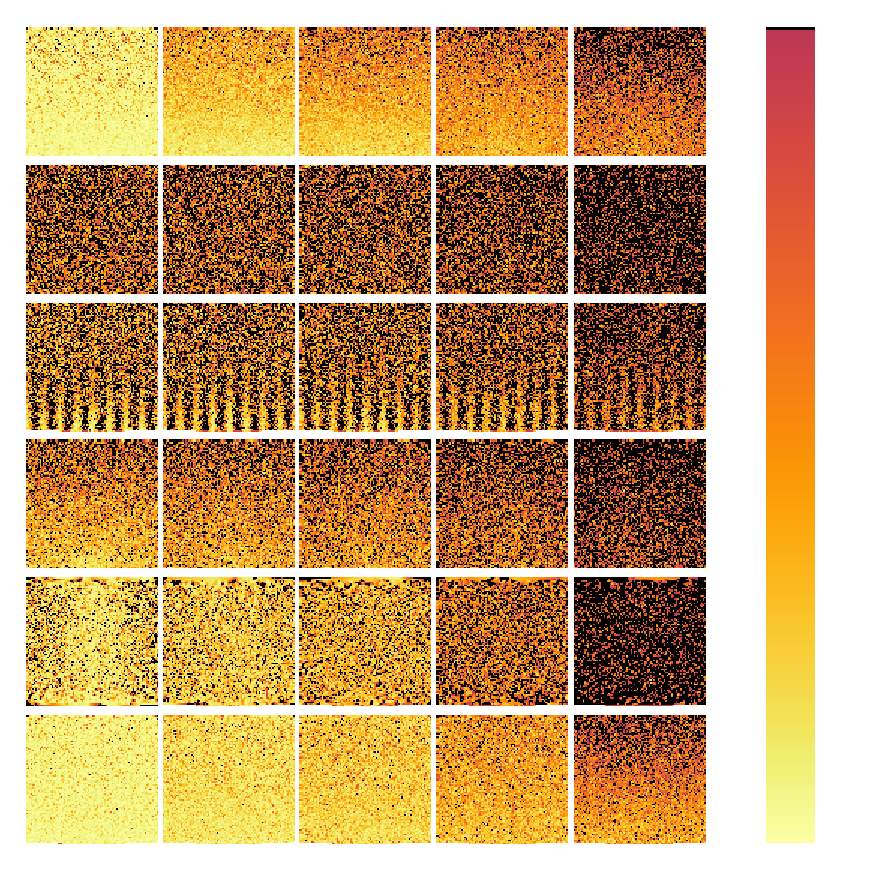
\includegraphics{./figures/parts/appendix/chapters/05/sections/04/caer_style_position_errors_dxyt2}}%
    \gplfronttext
  \end{picture}%
\endgroup

  \vspace{1cm}
  \caption{\small Χάρτες θερμότητας των μέτρων των τελικών σφαλμάτων εκτίμησης
           θέσης συναρτήσει των αρχικών σφαλμάτων εκτίμησης προσανατολισμού
           $\Delta\hat{\theta} \in
           [-\overline{\delta}_{\theta},+\overline{\delta}_{\theta}]$ (στον
           οριζόντιο άξονα) και των μέτρων των αρχικών σφαλμάτων εκτίμησης
           θέσης $\|\Delta \hat{\bm{l}}\|_2 \in [0, \sqrt{2}\cdot
           \overline{\delta}_{xy}]$ (στον κάθετο άξονα) για όλα τα
           διενεργηθέντα πειράματα, ανά αλγόριθμο και ανά τυπική απόκλιση
           διαταραχών του φυσικού αισθητήρα, για τη διάταξη με
           $(\overline{\delta}_{xy}, \overline{\delta}_{\theta}) = (0.10,
           0.070)$ [m,rad], εστιασμένοι στο διάστημα $[0,
           e_{xy,\text{avg}}^{\overline{\delta}_{xy},
           \overline{\delta}_{\theta}}]$, όπου με
           $e_{xy,\text{avg}}^{\overline{\delta}_{xy},
           \overline{\delta}_{\theta}}$ σημειώνεται ο μέσος όρος σφάλματος
           εκτίμησης στάσης όλων των μεθόδων, για κάθε επεξεργασθέν δείγμα, και
           κάθε τιμή τυπικής απόκλισης των διαταραχών που επιδρούν στις
           μετρήσεις του φυσικού αισθητήρα, για τη διαμόρφωση
           $(\overline{\delta}_{xy}, \overline{\delta}_{\theta})$.  Τιμές
           μέτρου σφάλματος εκτίμησης άνω του μέσου όρου σημειώνονται με μαύρο
           χρώμα}
  \label{fig:appendix_05_01:14}
\end{figure}
\begin{figure}\vspace{1cm}\hspace{0.5cm}
  % GNUPLOT: LaTeX picture with Postscript
\begingroup
  \makeatletter
  \providecommand\color[2][]{%
    \GenericError{(gnuplot) \space\space\space\@spaces}{%
      Package color not loaded in conjunction with
      terminal option `colourtext'%
    }{See the gnuplot documentation for explanation.%
    }{Either use 'blacktext' in gnuplot or load the package
      color.sty in LaTeX.}%
    \renewcommand\color[2][]{}%
  }%
  \providecommand\includegraphics[2][]{%
    \GenericError{(gnuplot) \space\space\space\@spaces}{%
      Package graphicx or graphics not loaded%
    }{See the gnuplot documentation for explanation.%
    }{The gnuplot epslatex terminal needs graphicx.sty or graphics.sty.}%
    \renewcommand\includegraphics[2][]{}%
  }%
  \providecommand\rotatebox[2]{#2}%
  \@ifundefined{ifGPcolor}{%
    \newif\ifGPcolor
    \GPcolorfalse
  }{}%
  \@ifundefined{ifGPblacktext}{%
    \newif\ifGPblacktext
    \GPblacktexttrue
  }{}%
  % define a \g@addto@macro without @ in the name:
  \let\gplgaddtomacro\g@addto@macro
  % define empty templates for all commands taking text:
  \gdef\gplfronttext{}%
  \gdef\gplfronttext{}%
  \makeatother
  \ifGPblacktext
    % no textcolor at all
    \def\colorrgb#1{}%
    \def\colorgray#1{}%
  \else
    % gray or color?
    \ifGPcolor
      \def\colorrgb#1{\color[rgb]{#1}}%
      \def\colorgray#1{\color[gray]{#1}}%
      \expandafter\def\csname LTw\endcsname{\color{white}}%
      \expandafter\def\csname LTb\endcsname{\color{black}}%
      \expandafter\def\csname LTa\endcsname{\color{black}}%
      \expandafter\def\csname LT0\endcsname{\color[rgb]{1,0,0}}%
      \expandafter\def\csname LT1\endcsname{\color[rgb]{0,1,0}}%
      \expandafter\def\csname LT2\endcsname{\color[rgb]{0,0,1}}%
      \expandafter\def\csname LT3\endcsname{\color[rgb]{1,0,1}}%
      \expandafter\def\csname LT4\endcsname{\color[rgb]{0,1,1}}%
      \expandafter\def\csname LT5\endcsname{\color[rgb]{1,1,0}}%
      \expandafter\def\csname LT6\endcsname{\color[rgb]{0,0,0}}%
      \expandafter\def\csname LT7\endcsname{\color[rgb]{1,0.3,0}}%
      \expandafter\def\csname LT8\endcsname{\color[rgb]{0.5,0.5,0.5}}%
    \else
      % gray
      \def\colorrgb#1{\color{black}}%
      \def\colorgray#1{\color[gray]{#1}}%
      \expandafter\def\csname LTw\endcsname{\color{white}}%
      \expandafter\def\csname LTb\endcsname{\color{black}}%
      \expandafter\def\csname LTa\endcsname{\color{black}}%
      \expandafter\def\csname LT0\endcsname{\color{black}}%
      \expandafter\def\csname LT1\endcsname{\color{black}}%
      \expandafter\def\csname LT2\endcsname{\color{black}}%
      \expandafter\def\csname LT3\endcsname{\color{black}}%
      \expandafter\def\csname LT4\endcsname{\color{black}}%
      \expandafter\def\csname LT5\endcsname{\color{black}}%
      \expandafter\def\csname LT6\endcsname{\color{black}}%
      \expandafter\def\csname LT7\endcsname{\color{black}}%
      \expandafter\def\csname LT8\endcsname{\color{black}}%
    \fi
  \fi
  \setlength{\unitlength}{0.0500bp}%
  \begin{picture}(8000.00,8000.00)%
     \gplgaddtomacro\gplfronttext{%
      \colorrgb{0.00,0.00,0.00}%
      \put(716,8200){\makebox(0,0){\strut{}\small $\sigma_R = 0.01$}}%
      \colorrgb{0.00,0.00,0.00}%
      \put(2029,8200){\makebox(0,0){\strut{}\small $\sigma_R = 0.03$}}%
      \colorrgb{0.00,0.00,0.00}%
      \put(3343,8200){\makebox(0,0){\strut{}\small $\sigma_R = 0.05$}}%
      \colorrgb{0.00,0.00,0.00}%
      \put(4656,8200){\makebox(0,0){\strut{}\small $\sigma_R = 0.10$}}%
      \colorrgb{0.00,0.00,0.00}%
      \put(5969,8200){\makebox(0,0){\strut{}\small $\sigma_R = 0.20$ [m]}}%
      \put(3333.33,8700){\makebox(0,0){\strut{}$(\overline{\delta}_{xy}, \overline{\delta}_\theta) = (0.15 \ \text{m}, 0.15 \ \text{rad})$}}
      \put(4000,9200){\makebox(0,0){\strut{}Τελικά σφάλματα εκτίμησης θέσης ως προς αρχικές συνθήκες μετατόπισης [m]}}
    }%
    \gplgaddtomacro\gplfronttext{%
      \colorrgb{0.00,0.00,0.00}%
      \put(-200,7333.33){\rotatebox{90}{\makebox(0,0){\strut{}\small PLICP}}}%
    }%
    \gplgaddtomacro\gplfronttext{%
      \colorrgb{0.00,0.00,0.00}%
      \put(-200,6000){\rotatebox{90}{\makebox(0,0){\strut{}\small NDT}}}%
    }%
    \gplgaddtomacro\gplfronttext{%
      \colorrgb{0.00,0.00,0.00}%
      \put(-200,4666.66){\rotatebox{90}{\makebox(0,0){\strut{}\small FastGICP}}}%
    }%
    \gplgaddtomacro\gplfronttext{%
      \colorrgb{0.00,0.00,0.00}%
      \put(-200,3333.33){\rotatebox{90}{\makebox(0,0){\strut{}\small FastVGICP}}}%
    }%
    \gplgaddtomacro\gplfronttext{%
      \colorrgb{0.00,0.00,0.00}%
      \put(-200,2000){\rotatebox{90}{\makebox(0,0){\strut{}\small NDT-PSO}}}%
    }%
    \gplgaddtomacro\gplfronttext{%
      \colorrgb{0.00,0.00,0.00}%
      \put(-200,666.66){\rotatebox{90}{\makebox(0,0){\strut{}\small \texttt{fsm}}}}%
    }%
    % dxyt3
    \gplgaddtomacro\gplfronttext{%
      \colorrgb{0.00,0.00,0.00}%
      \put(7800,80){\makebox(0,0)[l]{\strut{}$0.0$}}%
      \colorrgb{0.00,0.00,0.00}%
      \put(7800,1086){\makebox(0,0)[l]{\strut{}$0.01$}}%
      \colorrgb{0.00,0.00,0.00}%
      \put(7800,2092){\makebox(0,0)[l]{\strut{}$0.02$}}%
      \colorrgb{0.00,0.00,0.00}%
      \put(7800,3098){\makebox(0,0)[l]{\strut{}$0.03$}}%
      \colorrgb{0.00,0.00,0.00}%
      \put(7800,4104){\makebox(0,0)[l]{\strut{}$0.04$}}%
      \colorrgb{0.00,0.00,0.00}%
      \put(7800,5110){\makebox(0,0)[l]{\strut{}$0.05$}}%
      \colorrgb{0.00,0.00,0.00}%
      \put(7800,6116){\makebox(0,0)[l]{\strut{}$0.06$}}%
      \colorrgb{0.00,0.00,0.00}%
      \put(7800,7122){\makebox(0,0)[l]{\strut{}$0.07$}}%
      \colorrgb{0.00,0.00,0.00}%
      \put(7800,7919){\makebox(0,0)[l]{\strut{}$> e^{\overline{\delta}_{xy}, \overline{\delta}_\theta}_{xy,\text{avg}} =  0.0779$}}%
    }%
    \put(0,0){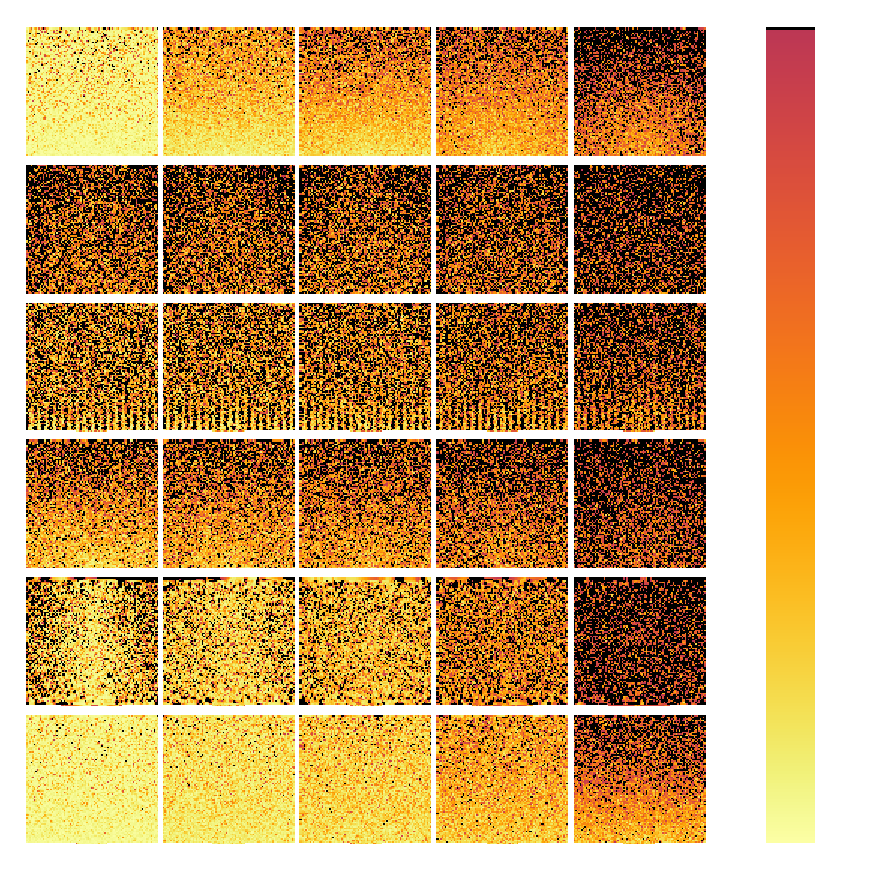
\includegraphics{./figures/parts/appendix/chapters/05/sections/03/caer_style_position_errors_dxyt3}}%
    \gplfronttext
  \end{picture}%
\endgroup

  \vspace{1cm}
  \caption{\small Χάρτες θερμότητας των μέτρων των τελικών σφαλμάτων εκτίμησης
           θέσης συναρτήσει των αρχικών σφαλμάτων εκτίμησης προσανατολισμού
           $\Delta\hat{\theta} \in
           [-\overline{\delta}_{\theta},+\overline{\delta}_{\theta}]$ (στον
           οριζόντιο άξονα) και των μέτρων των αρχικών σφαλμάτων εκτίμησης
           θέσης $\|\Delta \hat{\bm{l}}\|_2 \in [0, \sqrt{2}\cdot
           \overline{\delta}_{xy}]$ (στον κάθετο άξονα) για όλα τα
           διενεργηθέντα πειράματα, ανά αλγόριθμο και ανά τυπική απόκλιση
           διαταραχών του φυσικού αισθητήρα, για τη διάταξη με
           $(\overline{\delta}_{xy}, \overline{\delta}_{\theta}) = (0.15,
           0.150)$ [m,rad], εστιασμένοι στο διάστημα $[0,
           e_{xy,\text{avg}}^{\overline{\delta}_{xy},
           \overline{\delta}_{\theta}}]$, όπου με
           $e_{xy,\text{avg}}^{\overline{\delta}_{xy},
           \overline{\delta}_{\theta}}$ σημειώνεται ο μέσος όρος σφάλματος
           εκτίμησης στάσης όλων των μεθόδων, για κάθε επεξεργασθέν δείγμα, και
           κάθε τιμή τυπικής απόκλισης των διαταραχών που επιδρούν στις
           μετρήσεις του φυσικού αισθητήρα, για τη διαμόρφωση
           $(\overline{\delta}_{xy}, \overline{\delta}_{\theta})$.  Τιμές
           μέτρου σφάλματος εκτίμησης άνω του μέσου όρου σημειώνονται με μαύρο
           χρώμα}
  \label{fig:appendix_05_01:15}
\end{figure}
\begin{figure}\vspace{1cm}\hspace{0.5cm}
  % GNUPLOT: LaTeX picture with Postscript
\begingroup
  \makeatletter
  \providecommand\color[2][]{%
    \GenericError{(gnuplot) \space\space\space\@spaces}{%
      Package color not loaded in conjunction with
      terminal option `colourtext'%
    }{See the gnuplot documentation for explanation.%
    }{Either use 'blacktext' in gnuplot or load the package
      color.sty in LaTeX.}%
    \renewcommand\color[2][]{}%
  }%
  \providecommand\includegraphics[2][]{%
    \GenericError{(gnuplot) \space\space\space\@spaces}{%
      Package graphicx or graphics not loaded%
    }{See the gnuplot documentation for explanation.%
    }{The gnuplot epslatex terminal needs graphicx.sty or graphics.sty.}%
    \renewcommand\includegraphics[2][]{}%
  }%
  \providecommand\rotatebox[2]{#2}%
  \@ifundefined{ifGPcolor}{%
    \newif\ifGPcolor
    \GPcolorfalse
  }{}%
  \@ifundefined{ifGPblacktext}{%
    \newif\ifGPblacktext
    \GPblacktexttrue
  }{}%
  % define a \g@addto@macro without @ in the name:
  \let\gplgaddtomacro\g@addto@macro
  % define empty templates for all commands taking text:
  \gdef\gplfronttext{}%
  \gdef\gplfronttext{}%
  \makeatother
  \ifGPblacktext
    % no textcolor at all
    \def\colorrgb#1{}%
    \def\colorgray#1{}%
  \else
    % gray or color?
    \ifGPcolor
      \def\colorrgb#1{\color[rgb]{#1}}%
      \def\colorgray#1{\color[gray]{#1}}%
      \expandafter\def\csname LTw\endcsname{\color{white}}%
      \expandafter\def\csname LTb\endcsname{\color{black}}%
      \expandafter\def\csname LTa\endcsname{\color{black}}%
      \expandafter\def\csname LT0\endcsname{\color[rgb]{1,0,0}}%
      \expandafter\def\csname LT1\endcsname{\color[rgb]{0,1,0}}%
      \expandafter\def\csname LT2\endcsname{\color[rgb]{0,0,1}}%
      \expandafter\def\csname LT3\endcsname{\color[rgb]{1,0,1}}%
      \expandafter\def\csname LT4\endcsname{\color[rgb]{0,1,1}}%
      \expandafter\def\csname LT5\endcsname{\color[rgb]{1,1,0}}%
      \expandafter\def\csname LT6\endcsname{\color[rgb]{0,0,0}}%
      \expandafter\def\csname LT7\endcsname{\color[rgb]{1,0.3,0}}%
      \expandafter\def\csname LT8\endcsname{\color[rgb]{0.5,0.5,0.5}}%
    \else
      % gray
      \def\colorrgb#1{\color{black}}%
      \def\colorgray#1{\color[gray]{#1}}%
      \expandafter\def\csname LTw\endcsname{\color{white}}%
      \expandafter\def\csname LTb\endcsname{\color{black}}%
      \expandafter\def\csname LTa\endcsname{\color{black}}%
      \expandafter\def\csname LT0\endcsname{\color{black}}%
      \expandafter\def\csname LT1\endcsname{\color{black}}%
      \expandafter\def\csname LT2\endcsname{\color{black}}%
      \expandafter\def\csname LT3\endcsname{\color{black}}%
      \expandafter\def\csname LT4\endcsname{\color{black}}%
      \expandafter\def\csname LT5\endcsname{\color{black}}%
      \expandafter\def\csname LT6\endcsname{\color{black}}%
      \expandafter\def\csname LT7\endcsname{\color{black}}%
      \expandafter\def\csname LT8\endcsname{\color{black}}%
    \fi
  \fi
  \setlength{\unitlength}{0.0500bp}%
  \begin{picture}(8000.00,8000.00)%
     \gplgaddtomacro\gplfronttext{%
      \colorrgb{0.00,0.00,0.00}%
      \put(716,8200){\makebox(0,0){\strut{}\small $\sigma_R = 0.01$}}%
      \colorrgb{0.00,0.00,0.00}%
      \put(2029,8200){\makebox(0,0){\strut{}\small $\sigma_R = 0.03$}}%
      \colorrgb{0.00,0.00,0.00}%
      \put(3343,8200){\makebox(0,0){\strut{}\small $\sigma_R = 0.05$}}%
      \colorrgb{0.00,0.00,0.00}%
      \put(4656,8200){\makebox(0,0){\strut{}\small $\sigma_R = 0.10$}}%
      \colorrgb{0.00,0.00,0.00}%
      \put(5969,8200){\makebox(0,0){\strut{}\small $\sigma_R = 0.20$ [m]}}%
    }%
    \gplgaddtomacro\gplfronttext{%
      \colorrgb{0.00,0.00,0.00}%
      \put(-200,7333.33){\rotatebox{90}{\makebox(0,0){\strut{}\small PLICP}}}%
    }%
    \gplgaddtomacro\gplfronttext{%
      \colorrgb{0.00,0.00,0.00}%
      \put(-200,6000){\rotatebox{90}{\makebox(0,0){\strut{}\small NDT}}}%
    }%
    \gplgaddtomacro\gplfronttext{%
      \colorrgb{0.00,0.00,0.00}%
      \put(-200,4666.66){\rotatebox{90}{\makebox(0,0){\strut{}\small FastGICP}}}%
    }%
    \gplgaddtomacro\gplfronttext{%
      \colorrgb{0.00,0.00,0.00}%
      \put(-200,3333.33){\rotatebox{90}{\makebox(0,0){\strut{}\small FastVGICP}}}%
    }%
    \gplgaddtomacro\gplfronttext{%
      \colorrgb{0.00,0.00,0.00}%
      \put(-200,2000){\rotatebox{90}{\makebox(0,0){\strut{}\small NDT-PSO}}}%
    }%
    \gplgaddtomacro\gplfronttext{%
      \colorrgb{0.00,0.00,0.00}%
      \put(-200,666.66){\rotatebox{90}{\makebox(0,0){\strut{}\small \texttt{fsm}}}}%
    }%
    % dxyt4
    \gplgaddtomacro\gplfronttext{%
      \colorrgb{0.00,0.00,0.00}%
      \put(7800,80){\makebox(0,0)[l]{\strut{}$0.0$}}%
      \colorrgb{0.00,0.00,0.00}%
      \put(7800,1682){\makebox(0,0)[l]{\strut{}$0.02$}}%
      \colorrgb{0.00,0.00,0.00}%
      \put(7800,3284){\makebox(0,0)[l]{\strut{}$0.04$}}%
      \colorrgb{0.00,0.00,0.00}%
      \put(7800,4886){\makebox(0,0)[l]{\strut{}$0.06$}}%
      \colorrgb{0.00,0.00,0.00}%
      \put(7800,6488){\makebox(0,0)[l]{\strut{}$0.08$}}%
      \colorrgb{0.00,0.00,0.00}%
      \put(7800,7919){\makebox(0,0)[l]{\strut{}$> 0.097865$}}%
    }%
    \put(0,0){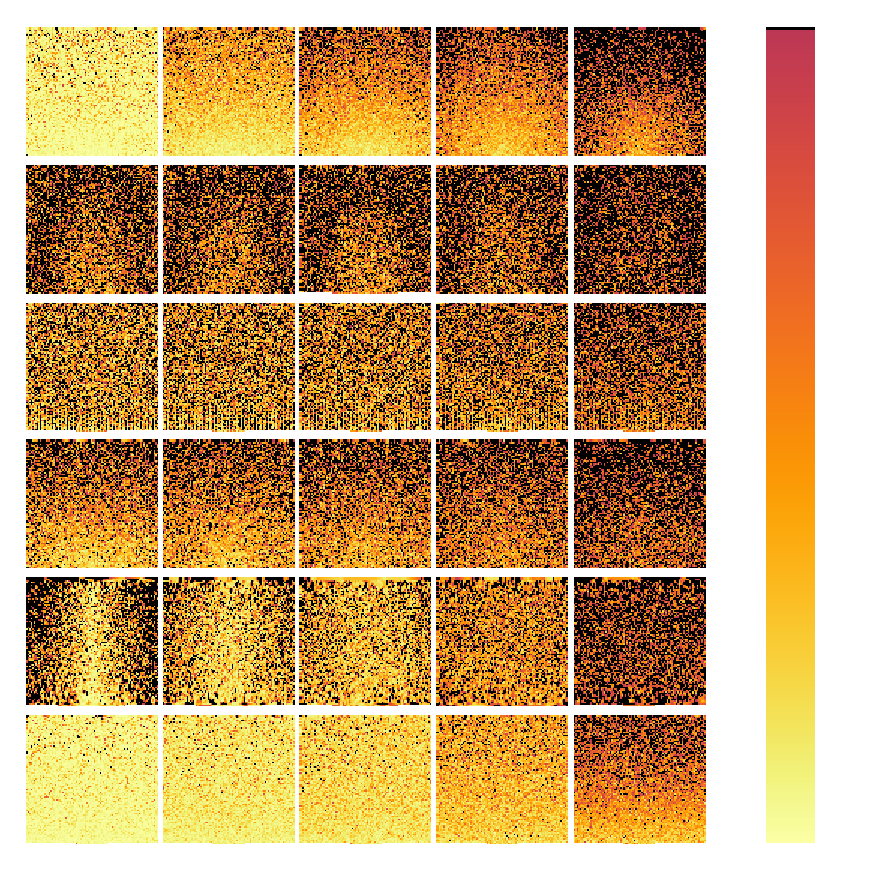
\includegraphics{./figures/parts/appendix/chapters/05/sections/04/caer_style_position_errors_dxyt4}}%
    \gplfronttext
  \end{picture}%
\endgroup

  \vspace{1cm}
  \caption{\small Χάρτες θερμότητας των μέτρων των τελικών σφαλμάτων εκτίμησης
           θέσης συναρτήσει των αρχικών σφαλμάτων εκτίμησης προσανατολισμού
           $\Delta\hat{\theta} \in
           [-\overline{\delta}_{\theta},+\overline{\delta}_{\theta}]$ (στον
           οριζόντιο άξονα) και των μέτρων των αρχικών σφαλμάτων εκτίμησης
           θέσης $\|\Delta \hat{\bm{l}}\|_2 \in [0, \sqrt{2}\cdot
           \overline{\delta}_{xy}]$ (στον κάθετο άξονα) για όλα τα
           διενεργηθέντα πειράματα, ανά αλγόριθμο και ανά τυπική απόκλιση
           διαταραχών του φυσικού αισθητήρα, για τη διάταξη με
           $(\overline{\delta}_{xy}, \overline{\delta}_{\theta}) = (0.20,
           0.30)$ [m,rad], εστιασμένοι στο διάστημα $[0,
           e_{xy,\text{avg}}^{\overline{\delta}_{xy},
           \overline{\delta}_{\theta}}]$, όπου με
           $e_{xy,\text{avg}}^{\overline{\delta}_{xy},
           \overline{\delta}_{\theta}}$ σημειώνεται ο μέσος όρος σφάλματος
           εκτίμησης στάσης όλων των μεθόδων, για κάθε επεξεργασθέν δείγμα, και
           κάθε τιμή τυπικής απόκλισης των διαταραχών που επιδρούν στις
           μετρήσεις του φυσικού αισθητήρα, για τη διαμόρφωση
           $(\overline{\delta}_{xy}, \overline{\delta}_{\theta})$.  Τιμές
           μέτρου σφάλματος εκτίμησης άνω του μέσου όρου σημειώνονται με μαύρο
           χρώμα}
  \label{fig:appendix_05_01:16}
\end{figure}
\begin{figure}\vspace{1cm}\hspace{0.5cm}
  % GNUPLOT: LaTeX picture with Postscript
\begingroup
  \makeatletter
  \providecommand\color[2][]{%
    \GenericError{(gnuplot) \space\space\space\@spaces}{%
      Package color not loaded in conjunction with
      terminal option `colourtext'%
    }{See the gnuplot documentation for explanation.%
    }{Either use 'blacktext' in gnuplot or load the package
      color.sty in LaTeX.}%
    \renewcommand\color[2][]{}%
  }%
  \providecommand\includegraphics[2][]{%
    \GenericError{(gnuplot) \space\space\space\@spaces}{%
      Package graphicx or graphics not loaded%
    }{See the gnuplot documentation for explanation.%
    }{The gnuplot epslatex terminal needs graphicx.sty or graphics.sty.}%
    \renewcommand\includegraphics[2][]{}%
  }%
  \providecommand\rotatebox[2]{#2}%
  \@ifundefined{ifGPcolor}{%
    \newif\ifGPcolor
    \GPcolorfalse
  }{}%
  \@ifundefined{ifGPblacktext}{%
    \newif\ifGPblacktext
    \GPblacktexttrue
  }{}%
  % define a \g@addto@macro without @ in the name:
  \let\gplgaddtomacro\g@addto@macro
  % define empty templates for all commands taking text:
  \gdef\gplfronttext{}%
  \gdef\gplfronttext{}%
  \makeatother
  \ifGPblacktext
    % no textcolor at all
    \def\colorrgb#1{}%
    \def\colorgray#1{}%
  \else
    % gray or color?
    \ifGPcolor
      \def\colorrgb#1{\color[rgb]{#1}}%
      \def\colorgray#1{\color[gray]{#1}}%
      \expandafter\def\csname LTw\endcsname{\color{white}}%
      \expandafter\def\csname LTb\endcsname{\color{black}}%
      \expandafter\def\csname LTa\endcsname{\color{black}}%
      \expandafter\def\csname LT0\endcsname{\color[rgb]{1,0,0}}%
      \expandafter\def\csname LT1\endcsname{\color[rgb]{0,1,0}}%
      \expandafter\def\csname LT2\endcsname{\color[rgb]{0,0,1}}%
      \expandafter\def\csname LT3\endcsname{\color[rgb]{1,0,1}}%
      \expandafter\def\csname LT4\endcsname{\color[rgb]{0,1,1}}%
      \expandafter\def\csname LT5\endcsname{\color[rgb]{1,1,0}}%
      \expandafter\def\csname LT6\endcsname{\color[rgb]{0,0,0}}%
      \expandafter\def\csname LT7\endcsname{\color[rgb]{1,0.3,0}}%
      \expandafter\def\csname LT8\endcsname{\color[rgb]{0.5,0.5,0.5}}%
    \else
      % gray
      \def\colorrgb#1{\color{black}}%
      \def\colorgray#1{\color[gray]{#1}}%
      \expandafter\def\csname LTw\endcsname{\color{white}}%
      \expandafter\def\csname LTb\endcsname{\color{black}}%
      \expandafter\def\csname LTa\endcsname{\color{black}}%
      \expandafter\def\csname LT0\endcsname{\color{black}}%
      \expandafter\def\csname LT1\endcsname{\color{black}}%
      \expandafter\def\csname LT2\endcsname{\color{black}}%
      \expandafter\def\csname LT3\endcsname{\color{black}}%
      \expandafter\def\csname LT4\endcsname{\color{black}}%
      \expandafter\def\csname LT5\endcsname{\color{black}}%
      \expandafter\def\csname LT6\endcsname{\color{black}}%
      \expandafter\def\csname LT7\endcsname{\color{black}}%
      \expandafter\def\csname LT8\endcsname{\color{black}}%
    \fi
  \fi
  \setlength{\unitlength}{0.0500bp}%
  \begin{picture}(8000.00,8000.00)%
     \gplgaddtomacro\gplfronttext{%
      \colorrgb{0.00,0.00,0.00}%
      \put(716,8200){\makebox(0,0){\strut{}\small $\sigma_R = 0.01$}}%
      \colorrgb{0.00,0.00,0.00}%
      \put(2029,8200){\makebox(0,0){\strut{}\small $\sigma_R = 0.03$}}%
      \colorrgb{0.00,0.00,0.00}%
      \put(3343,8200){\makebox(0,0){\strut{}\small $\sigma_R = 0.05$}}%
      \colorrgb{0.00,0.00,0.00}%
      \put(4656,8200){\makebox(0,0){\strut{}\small $\sigma_R = 0.10$}}%
      \colorrgb{0.00,0.00,0.00}%
      \put(5969,8200){\makebox(0,0){\strut{}\small $\sigma_R = 0.20$ [m]}}%
    }%
    \gplgaddtomacro\gplfronttext{%
      \colorrgb{0.00,0.00,0.00}%
      \put(-200,7333.33){\rotatebox{90}{\makebox(0,0){\strut{}\small PLICP}}}%
    }%
    \gplgaddtomacro\gplfronttext{%
      \colorrgb{0.00,0.00,0.00}%
      \put(-200,6000){\rotatebox{90}{\makebox(0,0){\strut{}\small NDT}}}%
    }%
    \gplgaddtomacro\gplfronttext{%
      \colorrgb{0.00,0.00,0.00}%
      \put(-200,4666.66){\rotatebox{90}{\makebox(0,0){\strut{}\small FastGICP}}}%
    }%
    \gplgaddtomacro\gplfronttext{%
      \colorrgb{0.00,0.00,0.00}%
      \put(-200,3333.33){\rotatebox{90}{\makebox(0,0){\strut{}\small FastVGICP}}}%
    }%
    \gplgaddtomacro\gplfronttext{%
      \colorrgb{0.00,0.00,0.00}%
      \put(-200,2000){\rotatebox{90}{\makebox(0,0){\strut{}\small NDT-PSO}}}%
    }%
    \gplgaddtomacro\gplfronttext{%
      \colorrgb{0.00,0.00,0.00}%
      \put(-200,666.66){\rotatebox{90}{\makebox(0,0){\strut{}\small \texttt{fsm}}}}%
    }%
    % dxyt5
    \gplgaddtomacro\gplfronttext{%
      \colorrgb{0.00,0.00,0.00}%
      \put(7800,80){\makebox(0,0)[l]{\strut{}$0.0$}}%
      \colorrgb{0.00,0.00,0.00}%
      \put(7800,1387){\makebox(0,0)[l]{\strut{}$0.02$}}%
      \colorrgb{0.00,0.00,0.00}%
      \put(7800,2694){\makebox(0,0)[l]{\strut{}$0.04$}}%
      \colorrgb{0.00,0.00,0.00}%
      \put(7800,4001){\makebox(0,0)[l]{\strut{}$0.06$}}%
      \colorrgb{0.00,0.00,0.00}%
      \put(7800,5309){\makebox(0,0)[l]{\strut{}$0.08$}}%
      \colorrgb{0.00,0.00,0.00}%
      \put(7800,6616){\makebox(0,0)[l]{\strut{}$0.10$}}%
      \colorrgb{0.00,0.00,0.00}%
      \put(7800,7919){\makebox(0,0)[l]{\strut{}$> 0.11994$}}%
    }%
    \put(0,0){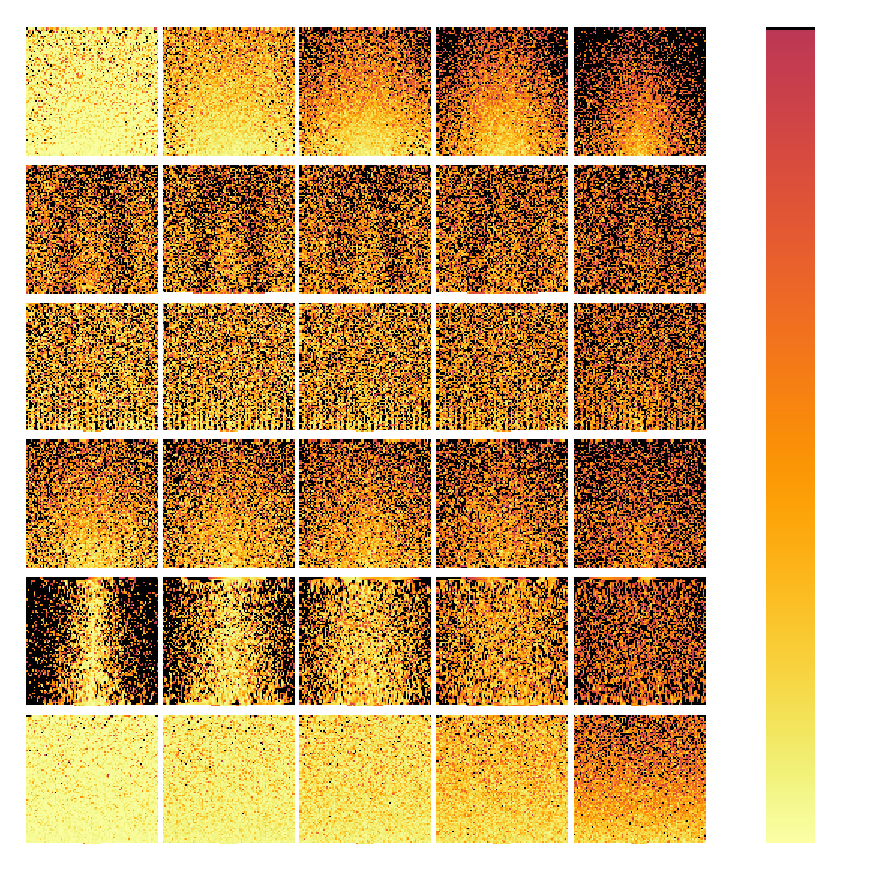
\includegraphics{./figures/parts/appendix/chapters/05/sections/04/caer_style_position_errors_dxyt5}}%
    \gplfronttext
  \end{picture}%
\endgroup

  \vspace{1cm}
  \caption{\small Χάρτες θερμότητας των μέτρων των τελικών σφαλμάτων εκτίμησης
           θέσης συναρτήσει των αρχικών σφαλμάτων εκτίμησης προσανατολισμού
           $\Delta\hat{\theta} \in
           [-\overline{\delta}_{\theta},+\overline{\delta}_{\theta}]$ (στον
           οριζόντιο άξονα) και των μέτρων των αρχικών σφαλμάτων εκτίμησης
           θέσης $\|\Delta \hat{\bm{l}}\|_2 \in [0, \sqrt{2}\cdot
           \overline{\delta}_{xy}]$ (στον κάθετο άξονα) για όλα τα
           διενεργηθέντα πειράματα, ανά αλγόριθμο και ανά τυπική απόκλιση
           διαταραχών του φυσικού αισθητήρα, για τη διάταξη με
           $(\overline{\delta}_{xy}, \overline{\delta}_{\theta}) = (0.20,
           0.56)$ [m,rad], εστιασμένοι στο διάστημα $[0,
           e_{xy,\text{avg}}^{\overline{\delta}_{xy},
           \overline{\delta}_{\theta}}]$, όπου με
           $e_{xy,\text{avg}}^{\overline{\delta}_{xy},
           \overline{\delta}_{\theta}}$ σημειώνεται ο μέσος όρος σφάλματος
           εκτίμησης στάσης όλων των μεθόδων, για κάθε επεξεργασθέν δείγμα, και
           κάθε τιμή τυπικής απόκλισης των διαταραχών που επιδρούν στις
           μετρήσεις του φυσικού αισθητήρα, για τη διαμόρφωση
           $(\overline{\delta}_{xy}, \overline{\delta}_{\theta})$.  Τιμές
           μέτρου σφάλματος εκτίμησης άνω του μέσου όρου σημειώνονται με μαύρο
           χρώμα}
  \label{fig:appendix_05_01:17}
\end{figure}
\begin{figure}\vspace{1cm}\hspace{0.5cm}
  % GNUPLOT: LaTeX picture with Postscript
\begingroup
  \makeatletter
  \providecommand\color[2][]{%
    \GenericError{(gnuplot) \space\space\space\@spaces}{%
      Package color not loaded in conjunction with
      terminal option `colourtext'%
    }{See the gnuplot documentation for explanation.%
    }{Either use 'blacktext' in gnuplot or load the package
      color.sty in LaTeX.}%
    \renewcommand\color[2][]{}%
  }%
  \providecommand\includegraphics[2][]{%
    \GenericError{(gnuplot) \space\space\space\@spaces}{%
      Package graphicx or graphics not loaded%
    }{See the gnuplot documentation for explanation.%
    }{The gnuplot epslatex terminal needs graphicx.sty or graphics.sty.}%
    \renewcommand\includegraphics[2][]{}%
  }%
  \providecommand\rotatebox[2]{#2}%
  \@ifundefined{ifGPcolor}{%
    \newif\ifGPcolor
    \GPcolorfalse
  }{}%
  \@ifundefined{ifGPblacktext}{%
    \newif\ifGPblacktext
    \GPblacktexttrue
  }{}%
  % define a \g@addto@macro without @ in the name:
  \let\gplgaddtomacro\g@addto@macro
  % define empty templates for all commands taking text:
  \gdef\gplfronttext{}%
  \gdef\gplfronttext{}%
  \makeatother
  \ifGPblacktext
    % no textcolor at all
    \def\colorrgb#1{}%
    \def\colorgray#1{}%
  \else
    % gray or color?
    \ifGPcolor
      \def\colorrgb#1{\color[rgb]{#1}}%
      \def\colorgray#1{\color[gray]{#1}}%
      \expandafter\def\csname LTw\endcsname{\color{white}}%
      \expandafter\def\csname LTb\endcsname{\color{black}}%
      \expandafter\def\csname LTa\endcsname{\color{black}}%
      \expandafter\def\csname LT0\endcsname{\color[rgb]{1,0,0}}%
      \expandafter\def\csname LT1\endcsname{\color[rgb]{0,1,0}}%
      \expandafter\def\csname LT2\endcsname{\color[rgb]{0,0,1}}%
      \expandafter\def\csname LT3\endcsname{\color[rgb]{1,0,1}}%
      \expandafter\def\csname LT4\endcsname{\color[rgb]{0,1,1}}%
      \expandafter\def\csname LT5\endcsname{\color[rgb]{1,1,0}}%
      \expandafter\def\csname LT6\endcsname{\color[rgb]{0,0,0}}%
      \expandafter\def\csname LT7\endcsname{\color[rgb]{1,0.3,0}}%
      \expandafter\def\csname LT8\endcsname{\color[rgb]{0.5,0.5,0.5}}%
    \else
      % gray
      \def\colorrgb#1{\color{black}}%
      \def\colorgray#1{\color[gray]{#1}}%
      \expandafter\def\csname LTw\endcsname{\color{white}}%
      \expandafter\def\csname LTb\endcsname{\color{black}}%
      \expandafter\def\csname LTa\endcsname{\color{black}}%
      \expandafter\def\csname LT0\endcsname{\color{black}}%
      \expandafter\def\csname LT1\endcsname{\color{black}}%
      \expandafter\def\csname LT2\endcsname{\color{black}}%
      \expandafter\def\csname LT3\endcsname{\color{black}}%
      \expandafter\def\csname LT4\endcsname{\color{black}}%
      \expandafter\def\csname LT5\endcsname{\color{black}}%
      \expandafter\def\csname LT6\endcsname{\color{black}}%
      \expandafter\def\csname LT7\endcsname{\color{black}}%
      \expandafter\def\csname LT8\endcsname{\color{black}}%
    \fi
  \fi
  \setlength{\unitlength}{0.0500bp}%
  \begin{picture}(8000.00,8000.00)%
     \gplgaddtomacro\gplfronttext{%
      \colorrgb{0.00,0.00,0.00}%
      \put(716,8200){\makebox(0,0){\strut{}\small $\sigma_R = 0.01$}}%
      \colorrgb{0.00,0.00,0.00}%
      \put(2029,8200){\makebox(0,0){\strut{}\small $\sigma_R = 0.03$}}%
      \colorrgb{0.00,0.00,0.00}%
      \put(3343,8200){\makebox(0,0){\strut{}\small $\sigma_R = 0.05$}}%
      \colorrgb{0.00,0.00,0.00}%
      \put(4656,8200){\makebox(0,0){\strut{}\small $\sigma_R = 0.10$}}%
      \colorrgb{0.00,0.00,0.00}%
      \put(5969,8200){\makebox(0,0){\strut{}\small $\sigma_R = 0.20$ [m]}}%
      \put(3333.33,8700){\makebox(0,0){\strut{}$(\overline{\delta}_{xy}, \overline{\delta}_\theta) = (0.20 \ \text{m}, \pi/4 \ \text{rad})$}}
      \put(4000,9200){\makebox(0,0){\strut{}Τελικά σφάλματα εκτίμησης θέσης ως προς αρχικές συνθήκες μετατόπισης [m]}}
    }%
    \gplgaddtomacro\gplfronttext{%
      \colorrgb{0.00,0.00,0.00}%
      \put(-200,7333.33){\rotatebox{90}{\makebox(0,0){\strut{}\small PLICP}}}%
    }%
    \gplgaddtomacro\gplfronttext{%
      \colorrgb{0.00,0.00,0.00}%
      \put(-200,6000){\rotatebox{90}{\makebox(0,0){\strut{}\small NDT}}}%
    }%
    \gplgaddtomacro\gplfronttext{%
      \colorrgb{0.00,0.00,0.00}%
      \put(-200,4666.66){\rotatebox{90}{\makebox(0,0){\strut{}\small FastGICP}}}%
    }%
    \gplgaddtomacro\gplfronttext{%
      \colorrgb{0.00,0.00,0.00}%
      \put(-200,3333.33){\rotatebox{90}{\makebox(0,0){\strut{}\small FastVGICP}}}%
    }%
    \gplgaddtomacro\gplfronttext{%
      \colorrgb{0.00,0.00,0.00}%
      \put(-200,2000){\rotatebox{90}{\makebox(0,0){\strut{}\small NDT-PSO}}}%
    }%
    \gplgaddtomacro\gplfronttext{%
      \colorrgb{0.00,0.00,0.00}%
      \put(-200,666.66){\rotatebox{90}{\makebox(0,0){\strut{}\small \texttt{fsm}}}}%
    }%

    % dxyt6
    \gplgaddtomacro\gplfronttext{%
      \colorrgb{0.00,0.00,0.00}%
      \put(7800,80){\makebox(0,0)[l]{\strut{}$0.0$}}%
      \colorrgb{0.00,0.00,0.00}%
      \put(7800,1144){\makebox(0,0)[l]{\strut{}$0.02$}}%
      \colorrgb{0.00,0.00,0.00}%
      \put(7800,2207){\makebox(0,0)[l]{\strut{}$0.04$}}%
      \colorrgb{0.00,0.00,0.00}%
      \put(7800,3271){\makebox(0,0)[l]{\strut{}$0.06$}}%
      \colorrgb{0.00,0.00,0.00}%
      \put(7800,4335){\makebox(0,0)[l]{\strut{}$0.08$}}%
      \colorrgb{0.00,0.00,0.00}%
      \put(7800,5399){\makebox(0,0)[l]{\strut{}$0.10$}}%
      \colorrgb{0.00,0.00,0.00}%
      \put(7800,6462){\makebox(0,0)[l]{\strut{}$0.12$}}%
      \colorrgb{0.00,0.00,0.00}%
      \put(7800,7919){\makebox(0,0)[l]{\strut{}$> e^{\overline{\delta}_{xy}, \overline{\delta}_\theta}_{xy,\text{avg}} = 0.147$}}%
    }%
    \put(0,0){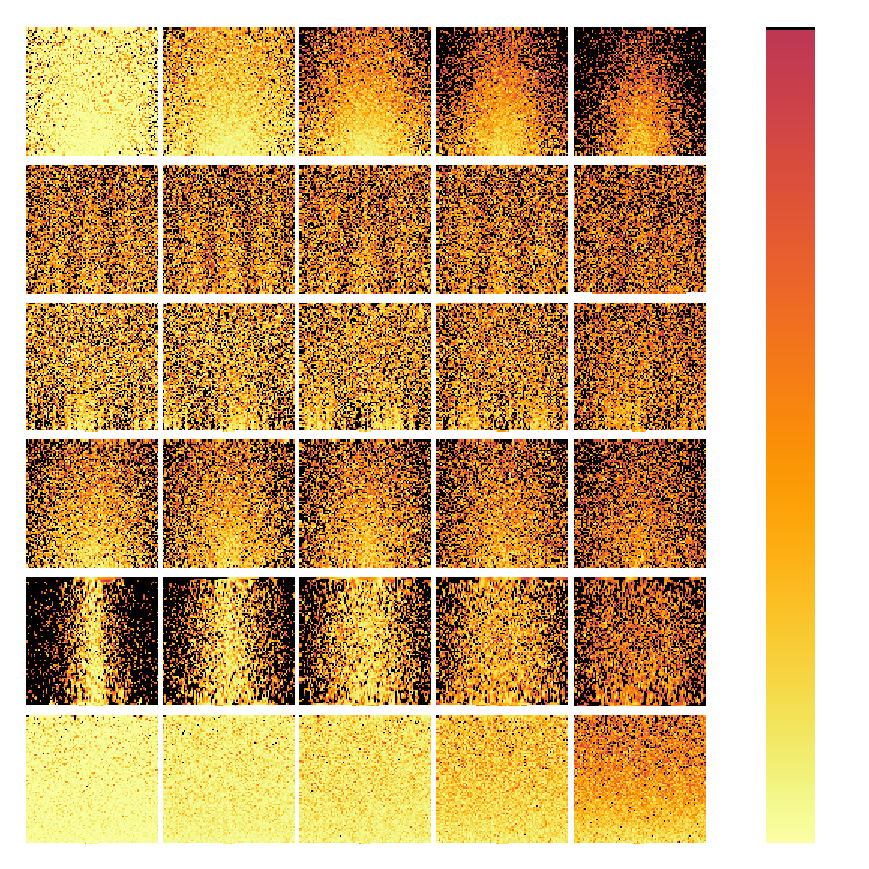
\includegraphics{./figures/parts/02/chapters/05/sections/04/caer_style_position_errors_dxyt6}}%
    \gplfronttext
  \end{picture}%
\endgroup

  \vspace{1cm}
  \caption{\small Χάρτες θερμότητας των μέτρων των τελικών σφαλμάτων εκτίμησης
           θέσης συναρτήσει των αρχικών σφαλμάτων εκτίμησης προσανατολισμού
           $\Delta\hat{\theta} \in
           [-\overline{\delta}_{\theta},+\overline{\delta}_{\theta}]$ (στον
           οριζόντιο άξονα) και των μέτρων των αρχικών σφαλμάτων εκτίμησης
           θέσης $\|\Delta \hat{\bm{l}}\|_2 \in [0, \sqrt{2}\cdot
           \overline{\delta}_{xy}]$ (στον κάθετο άξονα) για όλα τα
           διενεργηθέντα πειράματα, ανά αλγόριθμο και ανά τυπική απόκλιση
           διαταραχών του φυσικού αισθητήρα, για τη διάταξη με
           $(\overline{\delta}_{xy}, \overline{\delta}_{\theta}) = (0.20,
           \pi/4)$ [m,rad], εστιασμένοι στο διάστημα $[0,
           e_{xy,\text{avg}}^{\overline{\delta}_{xy},
           \overline{\delta}_{\theta}}]$, όπου με
           $e_{xy,\text{avg}}^{\overline{\delta}_{xy},
           \overline{\delta}_{\theta}}$ σημειώνεται ο μέσος όρος σφάλματος
           εκτίμησης στάσης όλων των μεθόδων, για κάθε επεξεργασθέν δείγμα, και
           κάθε τιμή τυπικής απόκλισης των διαταραχών που επιδρούν στις
           μετρήσεις του φυσικού αισθητήρα, για τη διαμόρφωση
           $(\overline{\delta}_{xy}, \overline{\delta}_{\theta})$.  Τιμές
           μέτρου σφάλματος εκτίμησης άνω του μέσου όρου σημειώνονται με μαύρο
           χρώμα}
  \label{fig:appendix_05_01:18}
\end{figure}


\begin{figure}\vspace{1cm}\hspace{0.5cm}
  % GNUPLOT: LaTeX picture with Postscript
\begingroup
  \makeatletter
  \providecommand\color[2][]{%
    \GenericError{(gnuplot) \space\space\space\@spaces}{%
      Package color not loaded in conjunction with
      terminal option `colourtext'%
    }{See the gnuplot documentation for explanation.%
    }{Either use 'blacktext' in gnuplot or load the package
      color.sty in LaTeX.}%
    \renewcommand\color[2][]{}%
  }%
  \providecommand\includegraphics[2][]{%
    \GenericError{(gnuplot) \space\space\space\@spaces}{%
      Package graphicx or graphics not loaded%
    }{See the gnuplot documentation for explanation.%
    }{The gnuplot epslatex terminal needs graphicx.sty or graphics.sty.}%
    \renewcommand\includegraphics[2][]{}%
  }%
  \providecommand\rotatebox[2]{#2}%
  \@ifundefined{ifGPcolor}{%
    \newif\ifGPcolor
    \GPcolorfalse
  }{}%
  \@ifundefined{ifGPblacktext}{%
    \newif\ifGPblacktext
    \GPblacktexttrue
  }{}%
  % define a \g@addto@macro without @ in the name:
  \let\gplgaddtomacro\g@addto@macro
  % define empty templates for all commands taking text:
  \gdef\gplfronttext{}%
  \gdef\gplfronttext{}%
  \makeatother
  \ifGPblacktext
    % no textcolor at all
    \def\colorrgb#1{}%
    \def\colorgray#1{}%
  \else
    % gray or color?
    \ifGPcolor
      \def\colorrgb#1{\color[rgb]{#1}}%
      \def\colorgray#1{\color[gray]{#1}}%
      \expandafter\def\csname LTw\endcsname{\color{white}}%
      \expandafter\def\csname LTb\endcsname{\color{black}}%
      \expandafter\def\csname LTa\endcsname{\color{black}}%
      \expandafter\def\csname LT0\endcsname{\color[rgb]{1,0,0}}%
      \expandafter\def\csname LT1\endcsname{\color[rgb]{0,1,0}}%
      \expandafter\def\csname LT2\endcsname{\color[rgb]{0,0,1}}%
      \expandafter\def\csname LT3\endcsname{\color[rgb]{1,0,1}}%
      \expandafter\def\csname LT4\endcsname{\color[rgb]{0,1,1}}%
      \expandafter\def\csname LT5\endcsname{\color[rgb]{1,1,0}}%
      \expandafter\def\csname LT6\endcsname{\color[rgb]{0,0,0}}%
      \expandafter\def\csname LT7\endcsname{\color[rgb]{1,0.3,0}}%
      \expandafter\def\csname LT8\endcsname{\color[rgb]{0.5,0.5,0.5}}%
    \else
      % gray
      \def\colorrgb#1{\color{black}}%
      \def\colorgray#1{\color[gray]{#1}}%
      \expandafter\def\csname LTw\endcsname{\color{white}}%
      \expandafter\def\csname LTb\endcsname{\color{black}}%
      \expandafter\def\csname LTa\endcsname{\color{black}}%
      \expandafter\def\csname LT0\endcsname{\color{black}}%
      \expandafter\def\csname LT1\endcsname{\color{black}}%
      \expandafter\def\csname LT2\endcsname{\color{black}}%
      \expandafter\def\csname LT3\endcsname{\color{black}}%
      \expandafter\def\csname LT4\endcsname{\color{black}}%
      \expandafter\def\csname LT5\endcsname{\color{black}}%
      \expandafter\def\csname LT6\endcsname{\color{black}}%
      \expandafter\def\csname LT7\endcsname{\color{black}}%
      \expandafter\def\csname LT8\endcsname{\color{black}}%
    \fi
  \fi
  \setlength{\unitlength}{0.0500bp}%
  \begin{picture}(8000.00,8000.00)%
     \gplgaddtomacro\gplfronttext{%
      \colorrgb{0.00,0.00,0.00}%
      \put(716,8200){\makebox(0,0){\strut{}\small $\sigma_R = 0.01$}}%
      \colorrgb{0.00,0.00,0.00}%
      \put(2029,8200){\makebox(0,0){\strut{}\small $\sigma_R = 0.03$}}%
      \colorrgb{0.00,0.00,0.00}%
      \put(3343,8200){\makebox(0,0){\strut{}\small $\sigma_R = 0.05$}}%
      \colorrgb{0.00,0.00,0.00}%
      \put(4656,8200){\makebox(0,0){\strut{}\small $\sigma_R = 0.10$}}%
      \colorrgb{0.00,0.00,0.00}%
      \put(5969,8200){\makebox(0,0){\strut{}\small $\sigma_R = 0.20$ [m]}}%
    }%
    \gplgaddtomacro\gplfronttext{%
      \colorrgb{0.00,0.00,0.00}%
      \put(-200,7333.33){\rotatebox{90}{\makebox(0,0){\strut{}\small PLICP}}}%
    }%
    \gplgaddtomacro\gplfronttext{%
      \colorrgb{0.00,0.00,0.00}%
      \put(-200,6000){\rotatebox{90}{\makebox(0,0){\strut{}\small NDT}}}%
    }%
    \gplgaddtomacro\gplfronttext{%
      \colorrgb{0.00,0.00,0.00}%
      \put(-200,4666.66){\rotatebox{90}{\makebox(0,0){\strut{}\small FastGICP}}}%
    }%
    \gplgaddtomacro\gplfronttext{%
      \colorrgb{0.00,0.00,0.00}%
      \put(-200,3333.33){\rotatebox{90}{\makebox(0,0){\strut{}\small FastVGICP}}}%
    }%
    \gplgaddtomacro\gplfronttext{%
      \colorrgb{0.00,0.00,0.00}%
      \put(-200,2000){\rotatebox{90}{\makebox(0,0){\strut{}\small NDT-PSO}}}%
    }%
    \gplgaddtomacro\gplfronttext{%
      \colorrgb{0.00,0.00,0.00}%
      \put(-200,666.66){\rotatebox{90}{\makebox(0,0){\strut{}\small \texttt{fsm}}}}%
    }%
    \gplgaddtomacro\gplfronttext{%
      \colorrgb{0.00,0.00,0.00}%
      \put(7800,80){\makebox(0,0)[l]{\strut{}$0.0$}}%
      \colorrgb{0.00,0.00,0.00}%
      \put(7800,2305){\makebox(0,0)[l]{\strut{}$0.005$}}%
      \colorrgb{0.00,0.00,0.00}%
      \put(7800,4530){\makebox(0,0)[l]{\strut{}$0.01$}}%
      \colorrgb{0.00,0.00,0.00}%
      \put(7800,6755){\makebox(0,0)[l]{\strut{}$0.015$}}%
      \colorrgb{0.00,0.00,0.00}%
      \put(7800,7919){\makebox(0,0)[l]{\strut{}$> 0.017615$}}%
    }%
    \put(0,0){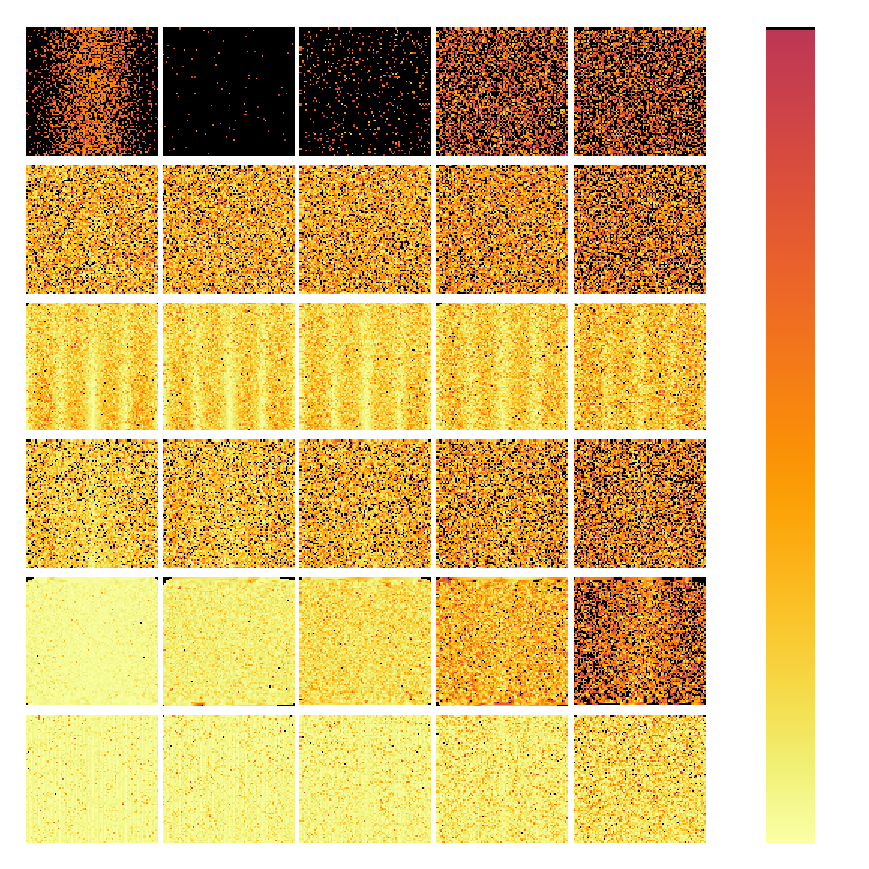
\includegraphics{./figures/parts/appendix/chapters/05/sections/04/caer_style_orientation_errors_dxyt1}}%
    \gplfronttext
  \end{picture}%
\endgroup

  \vspace{1cm}
  \caption{\small Χάρτες θερμότητας των μέτρων των τελικών σφαλμάτων εκτίμησης
           προσανατολισμού συναρτήσει των αρχικών σφαλμάτων εκτίμησης
           προσανατολισμού $\Delta\hat{\theta} \in
           [-\overline{\delta}_{\theta},+\overline{\delta}_{\theta}]$ (στον
           οριζόντιο άξονα) και των μέτρων των αρχικών σφαλμάτων εκτίμησης
           θέσης $\|\Delta \hat{\bm{l}}\|_2 \in [0, \sqrt{2}\cdot
           \overline{\delta}_{xy}]$ (στον κάθετο άξονα) για όλα τα
           διενεργηθέντα πειράματα, ανά αλγόριθμο και ανά τυπική απόκλιση
           διαταραχών του φυσικού αισθητήρα, για τη διάταξη με
           $(\overline{\delta}_{xy}, \overline{\delta}_{\theta}) = (0.05,
           0.035)$ [m,rad], εστιασμένοι στο διάστημα $[0,
           e_{xy,\text{avg}}^{\overline{\delta}_{xy},
           \overline{\delta}_{\theta}}]$, όπου με
           $e_{xy,\text{avg}}^{\overline{\delta}_{xy},
           \overline{\delta}_{\theta}}$ σημειώνεται ο μέσος όρος σφάλματος
           εκτίμησης στάσης όλων των μεθόδων, για κάθε επεξεργασθέν δείγμα, και
           κάθε τιμή τυπικής απόκλισης των διαταραχών που επιδρούν στις
           μετρήσεις του φυσικού αισθητήρα, για τη διαμόρφωση
           $(\overline{\delta}_{xy}, \overline{\delta}_{\theta})$.  Τιμές
           μέτρου σφάλματος εκτίμησης άνω του μέσου όρου σημειώνονται με μαύρο
           χρώμα}
  \label{fig:appendix_05_01:19}
\end{figure}
\begin{figure}\vspace{1cm}\hspace{0.5cm}
  % GNUPLOT: LaTeX picture with Postscript
\begingroup
  \makeatletter
  \providecommand\color[2][]{%
    \GenericError{(gnuplot) \space\space\space\@spaces}{%
      Package color not loaded in conjunction with
      terminal option `colourtext'%
    }{See the gnuplot documentation for explanation.%
    }{Either use 'blacktext' in gnuplot or load the package
      color.sty in LaTeX.}%
    \renewcommand\color[2][]{}%
  }%
  \providecommand\includegraphics[2][]{%
    \GenericError{(gnuplot) \space\space\space\@spaces}{%
      Package graphicx or graphics not loaded%
    }{See the gnuplot documentation for explanation.%
    }{The gnuplot epslatex terminal needs graphicx.sty or graphics.sty.}%
    \renewcommand\includegraphics[2][]{}%
  }%
  \providecommand\rotatebox[2]{#2}%
  \@ifundefined{ifGPcolor}{%
    \newif\ifGPcolor
    \GPcolorfalse
  }{}%
  \@ifundefined{ifGPblacktext}{%
    \newif\ifGPblacktext
    \GPblacktexttrue
  }{}%
  % define a \g@addto@macro without @ in the name:
  \let\gplgaddtomacro\g@addto@macro
  % define empty templates for all commands taking text:
  \gdef\gplfronttext{}%
  \gdef\gplfronttext{}%
  \makeatother
  \ifGPblacktext
    % no textcolor at all
    \def\colorrgb#1{}%
    \def\colorgray#1{}%
  \else
    % gray or color?
    \ifGPcolor
      \def\colorrgb#1{\color[rgb]{#1}}%
      \def\colorgray#1{\color[gray]{#1}}%
      \expandafter\def\csname LTw\endcsname{\color{white}}%
      \expandafter\def\csname LTb\endcsname{\color{black}}%
      \expandafter\def\csname LTa\endcsname{\color{black}}%
      \expandafter\def\csname LT0\endcsname{\color[rgb]{1,0,0}}%
      \expandafter\def\csname LT1\endcsname{\color[rgb]{0,1,0}}%
      \expandafter\def\csname LT2\endcsname{\color[rgb]{0,0,1}}%
      \expandafter\def\csname LT3\endcsname{\color[rgb]{1,0,1}}%
      \expandafter\def\csname LT4\endcsname{\color[rgb]{0,1,1}}%
      \expandafter\def\csname LT5\endcsname{\color[rgb]{1,1,0}}%
      \expandafter\def\csname LT6\endcsname{\color[rgb]{0,0,0}}%
      \expandafter\def\csname LT7\endcsname{\color[rgb]{1,0.3,0}}%
      \expandafter\def\csname LT8\endcsname{\color[rgb]{0.5,0.5,0.5}}%
    \else
      % gray
      \def\colorrgb#1{\color{black}}%
      \def\colorgray#1{\color[gray]{#1}}%
      \expandafter\def\csname LTw\endcsname{\color{white}}%
      \expandafter\def\csname LTb\endcsname{\color{black}}%
      \expandafter\def\csname LTa\endcsname{\color{black}}%
      \expandafter\def\csname LT0\endcsname{\color{black}}%
      \expandafter\def\csname LT1\endcsname{\color{black}}%
      \expandafter\def\csname LT2\endcsname{\color{black}}%
      \expandafter\def\csname LT3\endcsname{\color{black}}%
      \expandafter\def\csname LT4\endcsname{\color{black}}%
      \expandafter\def\csname LT5\endcsname{\color{black}}%
      \expandafter\def\csname LT6\endcsname{\color{black}}%
      \expandafter\def\csname LT7\endcsname{\color{black}}%
      \expandafter\def\csname LT8\endcsname{\color{black}}%
    \fi
  \fi
  \setlength{\unitlength}{0.0500bp}%
  \begin{picture}(8000.00,8000.00)%
     \gplgaddtomacro\gplfronttext{%
      \colorrgb{0.00,0.00,0.00}%
      \put(716,8200){\makebox(0,0){\strut{}\small $\sigma_R = 0.01$}}%
      \colorrgb{0.00,0.00,0.00}%
      \put(2029,8200){\makebox(0,0){\strut{}\small $\sigma_R = 0.03$}}%
      \colorrgb{0.00,0.00,0.00}%
      \put(3343,8200){\makebox(0,0){\strut{}\small $\sigma_R = 0.05$}}%
      \colorrgb{0.00,0.00,0.00}%
      \put(4656,8200){\makebox(0,0){\strut{}\small $\sigma_R = 0.10$}}%
      \colorrgb{0.00,0.00,0.00}%
      \put(5969,8200){\makebox(0,0){\strut{}\small $\sigma_R = 0.20$ [m]}}%
      \put(3333.33,8700){\makebox(0,0){\strut{}$(\overline{\delta}_{xy}, \overline{\delta}_\theta) = (0.10 \ \text{m}, 0.07 \ \text{rad})$}}
      \put(4000,9200){\makebox(0,0){\strut{}Τελικά σφάλματα εκτίμησης προσανατολισμού ως προς αρχικές συνθήκες μετατόπισης [rad]}}
    }%
    \gplgaddtomacro\gplfronttext{%
      \colorrgb{0.00,0.00,0.00}%
      \put(-200,7333.33){\rotatebox{90}{\makebox(0,0){\strut{}\small PLICP}}}%
    }%
    \gplgaddtomacro\gplfronttext{%
      \colorrgb{0.00,0.00,0.00}%
      \put(-200,6000){\rotatebox{90}{\makebox(0,0){\strut{}\small NDT}}}%
    }%
    \gplgaddtomacro\gplfronttext{%
      \colorrgb{0.00,0.00,0.00}%
      \put(-200,4666.66){\rotatebox{90}{\makebox(0,0){\strut{}\small FastGICP}}}%
    }%
    \gplgaddtomacro\gplfronttext{%
      \colorrgb{0.00,0.00,0.00}%
      \put(-200,3333.33){\rotatebox{90}{\makebox(0,0){\strut{}\small FastVGICP}}}%
    }%
    \gplgaddtomacro\gplfronttext{%
      \colorrgb{0.00,0.00,0.00}%
      \put(-200,2000){\rotatebox{90}{\makebox(0,0){\strut{}\small NDT-PSO}}}%
    }%
    \gplgaddtomacro\gplfronttext{%
      \colorrgb{0.00,0.00,0.00}%
      \put(-200,666.66){\rotatebox{90}{\makebox(0,0){\strut{}\small \texttt{fsm}}}}%
    }%
    \gplgaddtomacro\gplfronttext{%
      \colorrgb{0.00,0.00,0.00}%
      \put(7800,80){\makebox(0,0)[l]{\strut{}$0.0$}}%
      \colorrgb{0.00,0.00,0.00}%
      \put(7800,1984){\makebox(0,0)[l]{\strut{}$0.005$}}%
      \colorrgb{0.00,0.00,0.00}%
      \put(7800,3889){\makebox(0,0)[l]{\strut{}$0.01$}}%
      \colorrgb{0.00,0.00,0.00}%
      \put(7800,5793){\makebox(0,0)[l]{\strut{}$0.015$}}%
      \colorrgb{0.00,0.00,0.00}%
      \put(7800,7919){\makebox(0,0)[l]{\strut{}$> e^{\overline{\delta}_{xy}, \overline{\delta}_\theta}_{\theta,\text{avg}} = 0.0205$}}%
    }%
    \put(0,0){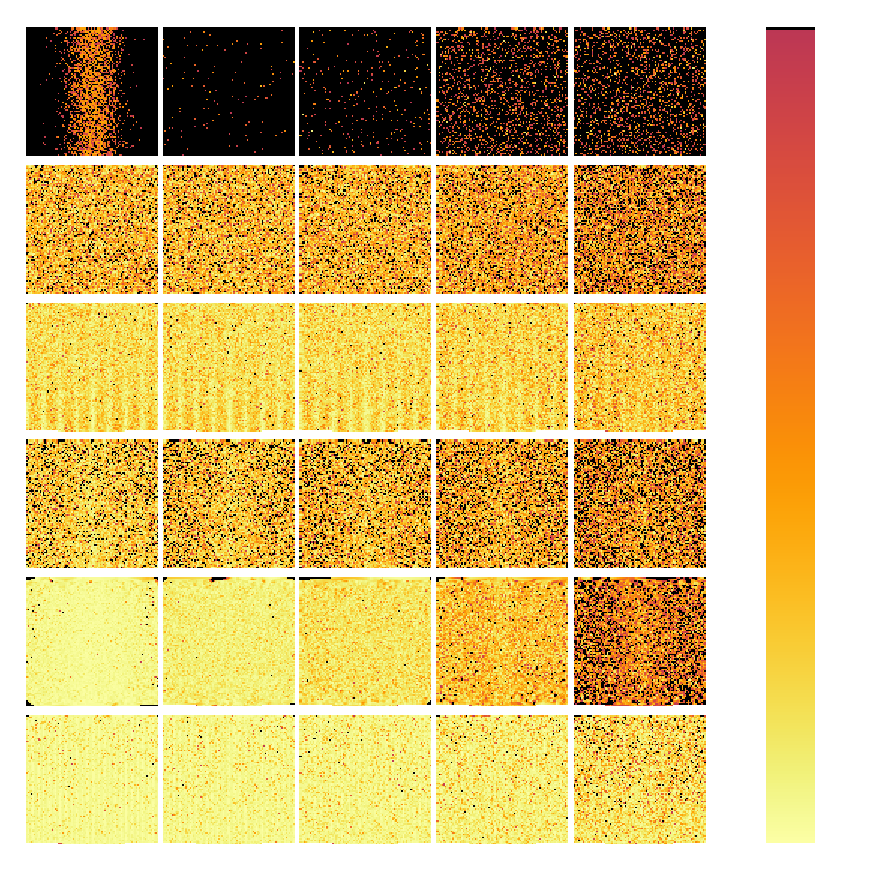
\includegraphics{./figures/parts/appendix/chapters/05/sections/04/caer_style_orientation_errors_dxyt2}}%
    \gplfronttext
  \end{picture}%
\endgroup

  \vspace{1cm}
  \caption{\small Χάρτες θερμότητας των μέτρων των τελικών σφαλμάτων εκτίμησης
           προσανατολισμού συναρτήσει των αρχικών σφαλμάτων εκτίμησης
           προσανατολισμού $\Delta\hat{\theta} \in
           [-\overline{\delta}_{\theta},+\overline{\delta}_{\theta}]$ (στον
           οριζόντιο άξονα) και των μέτρων των αρχικών σφαλμάτων εκτίμησης
           θέσης $\|\Delta \hat{\bm{l}}\|_2 \in [0, \sqrt{2}\cdot
           \overline{\delta}_{xy}]$ (στον κάθετο άξονα) για όλα τα
           διενεργηθέντα πειράματα, ανά αλγόριθμο και ανά τυπική απόκλιση
           διαταραχών του φυσικού αισθητήρα, για τη διάταξη με
           $(\overline{\delta}_{xy}, \overline{\delta}_{\theta}) = (0.10,
           0.070)$ [m,rad], εστιασμένοι στο διάστημα $[0,
           e_{xy,\text{avg}}^{\overline{\delta}_{xy},
           \overline{\delta}_{\theta}}]$, όπου με
           $e_{xy,\text{avg}}^{\overline{\delta}_{xy},
           \overline{\delta}_{\theta}}$ σημειώνεται ο μέσος όρος σφάλματος
           εκτίμησης στάσης όλων των μεθόδων, για κάθε επεξεργασθέν δείγμα, και
           κάθε τιμή τυπικής απόκλισης των διαταραχών που επιδρούν στις
           μετρήσεις του φυσικού αισθητήρα, για τη διαμόρφωση
           $(\overline{\delta}_{xy}, \overline{\delta}_{\theta})$.  Τιμές
           μέτρου σφάλματος εκτίμησης άνω του μέσου όρου σημειώνονται με μαύρο
           χρώμα}
  \label{fig:appendix_05_01:20}
\end{figure}
\begin{figure}\vspace{1cm}\hspace{0.5cm}
  % GNUPLOT: LaTeX picture with Postscript
\begingroup
  \makeatletter
  \providecommand\color[2][]{%
    \GenericError{(gnuplot) \space\space\space\@spaces}{%
      Package color not loaded in conjunction with
      terminal option `colourtext'%
    }{See the gnuplot documentation for explanation.%
    }{Either use 'blacktext' in gnuplot or load the package
      color.sty in LaTeX.}%
    \renewcommand\color[2][]{}%
  }%
  \providecommand\includegraphics[2][]{%
    \GenericError{(gnuplot) \space\space\space\@spaces}{%
      Package graphicx or graphics not loaded%
    }{See the gnuplot documentation for explanation.%
    }{The gnuplot epslatex terminal needs graphicx.sty or graphics.sty.}%
    \renewcommand\includegraphics[2][]{}%
  }%
  \providecommand\rotatebox[2]{#2}%
  \@ifundefined{ifGPcolor}{%
    \newif\ifGPcolor
    \GPcolorfalse
  }{}%
  \@ifundefined{ifGPblacktext}{%
    \newif\ifGPblacktext
    \GPblacktexttrue
  }{}%
  % define a \g@addto@macro without @ in the name:
  \let\gplgaddtomacro\g@addto@macro
  % define empty templates for all commands taking text:
  \gdef\gplbacktext{}%
  \gdef\gplfronttext{}%
  \makeatother
  \ifGPblacktext
    % no textcolor at all
    \def\colorrgb#1{}%
    \def\colorgray#1{}%
  \else
    % gray or color?
    \ifGPcolor
      \def\colorrgb#1{\color[rgb]{#1}}%
      \def\colorgray#1{\color[gray]{#1}}%
      \expandafter\def\csname LTw\endcsname{\color{white}}%
      \expandafter\def\csname LTb\endcsname{\color{black}}%
      \expandafter\def\csname LTa\endcsname{\color{black}}%
      \expandafter\def\csname LT0\endcsname{\color[rgb]{1,0,0}}%
      \expandafter\def\csname LT1\endcsname{\color[rgb]{0,1,0}}%
      \expandafter\def\csname LT2\endcsname{\color[rgb]{0,0,1}}%
      \expandafter\def\csname LT3\endcsname{\color[rgb]{1,0,1}}%
      \expandafter\def\csname LT4\endcsname{\color[rgb]{0,1,1}}%
      \expandafter\def\csname LT5\endcsname{\color[rgb]{1,1,0}}%
      \expandafter\def\csname LT6\endcsname{\color[rgb]{0,0,0}}%
      \expandafter\def\csname LT7\endcsname{\color[rgb]{1,0.3,0}}%
      \expandafter\def\csname LT8\endcsname{\color[rgb]{0.5,0.5,0.5}}%
    \else
      % gray
      \def\colorrgb#1{\color{black}}%
      \def\colorgray#1{\color[gray]{#1}}%
      \expandafter\def\csname LTw\endcsname{\color{white}}%
      \expandafter\def\csname LTb\endcsname{\color{black}}%
      \expandafter\def\csname LTa\endcsname{\color{black}}%
      \expandafter\def\csname LT0\endcsname{\color{black}}%
      \expandafter\def\csname LT1\endcsname{\color{black}}%
      \expandafter\def\csname LT2\endcsname{\color{black}}%
      \expandafter\def\csname LT3\endcsname{\color{black}}%
      \expandafter\def\csname LT4\endcsname{\color{black}}%
      \expandafter\def\csname LT5\endcsname{\color{black}}%
      \expandafter\def\csname LT6\endcsname{\color{black}}%
      \expandafter\def\csname LT7\endcsname{\color{black}}%
      \expandafter\def\csname LT8\endcsname{\color{black}}%
    \fi
  \fi
  \setlength{\unitlength}{0.0500bp}%
  \begin{picture}(8000.00,8000.00)%
     \gplgaddtomacro\gplfronttext{%
      \colorrgb{0.00,0.00,0.00}%
      \put(716,8200){\makebox(0,0){\strut{}\small $\sigma_R = 0.01$}}%
      \colorrgb{0.00,0.00,0.00}%
      \put(2029,8200){\makebox(0,0){\strut{}\small $\sigma_R = 0.03$}}%
      \colorrgb{0.00,0.00,0.00}%
      \put(3343,8200){\makebox(0,0){\strut{}\small $\sigma_R = 0.05$}}%
      \colorrgb{0.00,0.00,0.00}%
      \put(4656,8200){\makebox(0,0){\strut{}\small $\sigma_R = 0.10$}}%
      \colorrgb{0.00,0.00,0.00}%
      \put(5969,8200){\makebox(0,0){\strut{}\small $\sigma_R = 0.20$ [m]}}%
    }%
    \gplgaddtomacro\gplfronttext{%
      \colorrgb{0.00,0.00,0.00}%
      \put(-200,7333.33){\rotatebox{90}{\makebox(0,0){\strut{}\small PLICP}}}%
    }%
    \gplgaddtomacro\gplfronttext{%
      \colorrgb{0.00,0.00,0.00}%
      \put(-200,6000){\rotatebox{90}{\makebox(0,0){\strut{}\small NDT}}}%
    }%
    \gplgaddtomacro\gplfronttext{%
      \colorrgb{0.00,0.00,0.00}%
      \put(-200,4666.66){\rotatebox{90}{\makebox(0,0){\strut{}\small FastGICP}}}%
    }%
    \gplgaddtomacro\gplfronttext{%
      \colorrgb{0.00,0.00,0.00}%
      \put(-200,3333.33){\rotatebox{90}{\makebox(0,0){\strut{}\small FastVGICP}}}%
    }%
    \gplgaddtomacro\gplfronttext{%
      \colorrgb{0.00,0.00,0.00}%
      \put(-200,2000){\rotatebox{90}{\makebox(0,0){\strut{}\small NDT-PSO}}}%
    }%
    \gplgaddtomacro\gplfronttext{%
      \colorrgb{0.00,0.00,0.00}%
      \put(-200,666.66){\rotatebox{90}{\makebox(0,0){\strut{}\small \texttt{fsm}}}}%
    }%
    \gplgaddtomacro\gplfronttext{%
      \colorrgb{0.00,0.00,0.00}%
      \put(7800,80){\makebox(0,0)[l]{\strut{}$0.0$}}%
      \colorrgb{0.00,0.00,0.00}%
      \put(7800,1415){\makebox(0,0)[l]{\strut{}$0.005$}}%
      \colorrgb{0.00,0.00,0.00}%
      \put(7800,2750){\makebox(0,0)[l]{\strut{}$0.01$}}%
      \colorrgb{0.00,0.00,0.00}%
      \put(7800,4085){\makebox(0,0)[l]{\strut{}$0.015$}}%
      \colorrgb{0.00,0.00,0.00}%
      \put(7800,5420){\makebox(0,0)[l]{\strut{}$0.02$}}%
      \colorrgb{0.00,0.00,0.00}%
      \put(7800,6755){\makebox(0,0)[l]{\strut{}$0.025$}}%
      \colorrgb{0.00,0.00,0.00}%
      \put(7800,7919){\makebox(0,0)[l]{\strut{}$>  0.029359$}}%
    }%
    \put(0,0){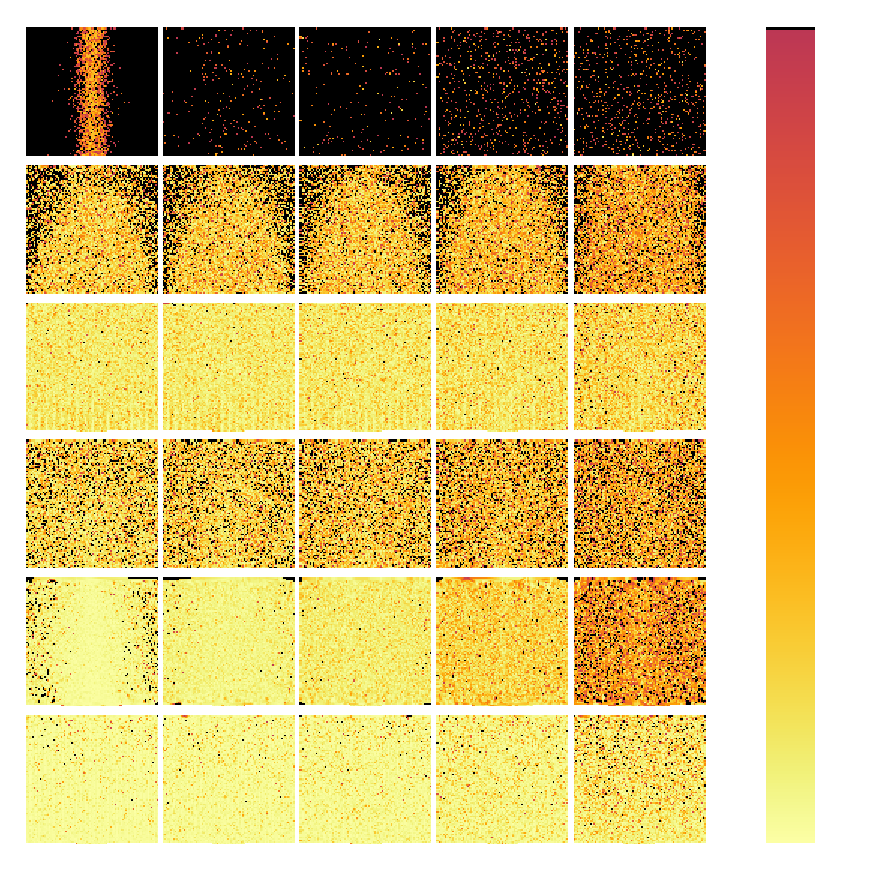
\includegraphics{./figures/parts/appendix/chapters/05/sections/04/caer_style_orientation_errors_dxyt3}}%
    \gplfronttext
  \end{picture}%
\endgroup

  \vspace{1cm}
  \caption{\small Χάρτες θερμότητας των μέτρων των τελικών σφαλμάτων εκτίμησης
           προσανατολισμού συναρτήσει των αρχικών σφαλμάτων εκτίμησης
           προσανατολισμού $\Delta\hat{\theta} \in
           [-\overline{\delta}_{\theta},+\overline{\delta}_{\theta}]$ (στον
           οριζόντιο άξονα) και των μέτρων των αρχικών σφαλμάτων εκτίμησης
           θέσης $\|\Delta \hat{\bm{l}}\|_2 \in [0, \sqrt{2}\cdot
           \overline{\delta}_{xy}]$ (στον κάθετο άξονα) για όλα τα
           διενεργηθέντα πειράματα, ανά αλγόριθμο και ανά τυπική απόκλιση
           διαταραχών του φυσικού αισθητήρα, για τη διάταξη με
           $(\overline{\delta}_{xy}, \overline{\delta}_{\theta}) = (0.15,
           0.150)$ [m,rad], εστιασμένοι στο διάστημα $[0,
           e_{xy,\text{avg}}^{\overline{\delta}_{xy},
           \overline{\delta}_{\theta}}]$, όπου με
           $e_{xy,\text{avg}}^{\overline{\delta}_{xy},
           \overline{\delta}_{\theta}}$ σημειώνεται ο μέσος όρος σφάλματος
           εκτίμησης στάσης όλων των μεθόδων, για κάθε επεξεργασθέν δείγμα, και
           κάθε τιμή τυπικής απόκλισης των διαταραχών που επιδρούν στις
           μετρήσεις του φυσικού αισθητήρα, για τη διαμόρφωση
           $(\overline{\delta}_{xy}, \overline{\delta}_{\theta})$.  Τιμές
           μέτρου σφάλματος εκτίμησης άνω του μέσου όρου σημειώνονται με μαύρο
           χρώμα}
  \label{fig:appendix_05_01:21}
\end{figure}
\begin{figure}\vspace{1cm}\hspace{0.5cm}
  % GNUPLOT: LaTeX picture with Postscript
\begingroup
  \makeatletter
  \providecommand\color[2][]{%
    \GenericError{(gnuplot) \space\space\space\@spaces}{%
      Package color not loaded in conjunction with
      terminal option `colourtext'%
    }{See the gnuplot documentation for explanation.%
    }{Either use 'blacktext' in gnuplot or load the package
      color.sty in LaTeX.}%
    \renewcommand\color[2][]{}%
  }%
  \providecommand\includegraphics[2][]{%
    \GenericError{(gnuplot) \space\space\space\@spaces}{%
      Package graphicx or graphics not loaded%
    }{See the gnuplot documentation for explanation.%
    }{The gnuplot epslatex terminal needs graphicx.sty or graphics.sty.}%
    \renewcommand\includegraphics[2][]{}%
  }%
  \providecommand\rotatebox[2]{#2}%
  \@ifundefined{ifGPcolor}{%
    \newif\ifGPcolor
    \GPcolorfalse
  }{}%
  \@ifundefined{ifGPblacktext}{%
    \newif\ifGPblacktext
    \GPblacktexttrue
  }{}%
  % define a \g@addto@macro without @ in the name:
  \let\gplgaddtomacro\g@addto@macro
  % define empty templates for all commands taking text:
  \gdef\gplfronttext{}%
  \gdef\gplfronttext{}%
  \makeatother
  \ifGPblacktext
    % no textcolor at all
    \def\colorrgb#1{}%
    \def\colorgray#1{}%
  \else
    % gray or color?
    \ifGPcolor
      \def\colorrgb#1{\color[rgb]{#1}}%
      \def\colorgray#1{\color[gray]{#1}}%
      \expandafter\def\csname LTw\endcsname{\color{white}}%
      \expandafter\def\csname LTb\endcsname{\color{black}}%
      \expandafter\def\csname LTa\endcsname{\color{black}}%
      \expandafter\def\csname LT0\endcsname{\color[rgb]{1,0,0}}%
      \expandafter\def\csname LT1\endcsname{\color[rgb]{0,1,0}}%
      \expandafter\def\csname LT2\endcsname{\color[rgb]{0,0,1}}%
      \expandafter\def\csname LT3\endcsname{\color[rgb]{1,0,1}}%
      \expandafter\def\csname LT4\endcsname{\color[rgb]{0,1,1}}%
      \expandafter\def\csname LT5\endcsname{\color[rgb]{1,1,0}}%
      \expandafter\def\csname LT6\endcsname{\color[rgb]{0,0,0}}%
      \expandafter\def\csname LT7\endcsname{\color[rgb]{1,0.3,0}}%
      \expandafter\def\csname LT8\endcsname{\color[rgb]{0.5,0.5,0.5}}%
    \else
      % gray
      \def\colorrgb#1{\color{black}}%
      \def\colorgray#1{\color[gray]{#1}}%
      \expandafter\def\csname LTw\endcsname{\color{white}}%
      \expandafter\def\csname LTb\endcsname{\color{black}}%
      \expandafter\def\csname LTa\endcsname{\color{black}}%
      \expandafter\def\csname LT0\endcsname{\color{black}}%
      \expandafter\def\csname LT1\endcsname{\color{black}}%
      \expandafter\def\csname LT2\endcsname{\color{black}}%
      \expandafter\def\csname LT3\endcsname{\color{black}}%
      \expandafter\def\csname LT4\endcsname{\color{black}}%
      \expandafter\def\csname LT5\endcsname{\color{black}}%
      \expandafter\def\csname LT6\endcsname{\color{black}}%
      \expandafter\def\csname LT7\endcsname{\color{black}}%
      \expandafter\def\csname LT8\endcsname{\color{black}}%
    \fi
  \fi
  \setlength{\unitlength}{0.0500bp}%
  \begin{picture}(8000.00,8000.00)%
     \gplgaddtomacro\gplfronttext{%
      \colorrgb{0.00,0.00,0.00}%
      \put(716,8200){\makebox(0,0){\strut{}\small $\sigma_R = 0.01$}}%
      \colorrgb{0.00,0.00,0.00}%
      \put(2029,8200){\makebox(0,0){\strut{}\small $\sigma_R = 0.03$}}%
      \colorrgb{0.00,0.00,0.00}%
      \put(3343,8200){\makebox(0,0){\strut{}\small $\sigma_R = 0.05$}}%
      \colorrgb{0.00,0.00,0.00}%
      \put(4656,8200){\makebox(0,0){\strut{}\small $\sigma_R = 0.10$}}%
      \colorrgb{0.00,0.00,0.00}%
      \put(5969,8200){\makebox(0,0){\strut{}\small $\sigma_R = 0.20$ [m]}}%
      \put(3333.33,8700){\makebox(0,0){\strut{}$(\overline{\delta}_{xy}, \overline{\delta}_\theta) = (0.20 \ \text{m}, 0.30 \ \text{rad})$}}
      \put(4000,9200){\makebox(0,0){\strut{}Τελικά σφάλματα εκτίμησης προσανατολισμού ως προς αρχικές συνθήκες μετατόπισης [rad]}}
    }%
    \gplgaddtomacro\gplfronttext{%
      \colorrgb{0.00,0.00,0.00}%
      \put(-200,7333.33){\rotatebox{90}{\makebox(0,0){\strut{}\small PLICP}}}%
    }%
    \gplgaddtomacro\gplfronttext{%
      \colorrgb{0.00,0.00,0.00}%
      \put(-200,6000){\rotatebox{90}{\makebox(0,0){\strut{}\small NDT}}}%
    }%
    \gplgaddtomacro\gplfronttext{%
      \colorrgb{0.00,0.00,0.00}%
      \put(-200,4666.66){\rotatebox{90}{\makebox(0,0){\strut{}\small FastGICP}}}%
    }%
    \gplgaddtomacro\gplfronttext{%
      \colorrgb{0.00,0.00,0.00}%
      \put(-200,3333.33){\rotatebox{90}{\makebox(0,0){\strut{}\small FastVGICP}}}%
    }%
    \gplgaddtomacro\gplfronttext{%
      \colorrgb{0.00,0.00,0.00}%
      \put(-200,2000){\rotatebox{90}{\makebox(0,0){\strut{}\small NDT-PSO}}}%
    }%
    \gplgaddtomacro\gplfronttext{%
      \colorrgb{0.00,0.00,0.00}%
      \put(-200,666.66){\rotatebox{90}{\makebox(0,0){\strut{}\small \texttt{fsm}}}}%
    }%
    \gplgaddtomacro\gplfronttext{%
      \colorrgb{0.00,0.00,0.00}%
      \put(7800,80){\makebox(0,0)[l]{\strut{}$0.0$}}%
      \colorrgb{0.00,0.00,0.00}%
      \put(7800,886){\makebox(0,0)[l]{\strut{}$0.005$}}%
      \colorrgb{0.00,0.00,0.00}%
      \put(7800,1692){\makebox(0,0)[l]{\strut{}$0.01$}}%
      \colorrgb{0.00,0.00,0.00}%
      \put(7800,2497){\makebox(0,0)[l]{\strut{}$0.015$}}%
      \colorrgb{0.00,0.00,0.00}%
      \put(7800,3303){\makebox(0,0)[l]{\strut{}$0.02$}}%
      \colorrgb{0.00,0.00,0.00}%
      \put(7800,4109){\makebox(0,0)[l]{\strut{}$0.025$}}%
      \colorrgb{0.00,0.00,0.00}%
      \put(7800,4915){\makebox(0,0)[l]{\strut{}$0.03$}}%
      \colorrgb{0.00,0.00,0.00}%
      \put(7800,5721){\makebox(0,0)[l]{\strut{}$0.035$}}%
      \colorrgb{0.00,0.00,0.00}%
      \put(7800,6527){\makebox(0,0)[l]{\strut{}$0.04$}}%
      \colorrgb{0.00,0.00,0.00}%
      \put(7800,7332){\makebox(0,0)[l]{\strut{}$0.045$}}%
      \colorrgb{0.00,0.00,0.00}%
      \put(7800,7919){\makebox(0,0)[l]{\strut{}$> e^{\overline{\delta}_{xy}, \overline{\delta}_\theta}_{\theta,\text{avg}} = 0.0486$}}%
    }%
    \put(0,0){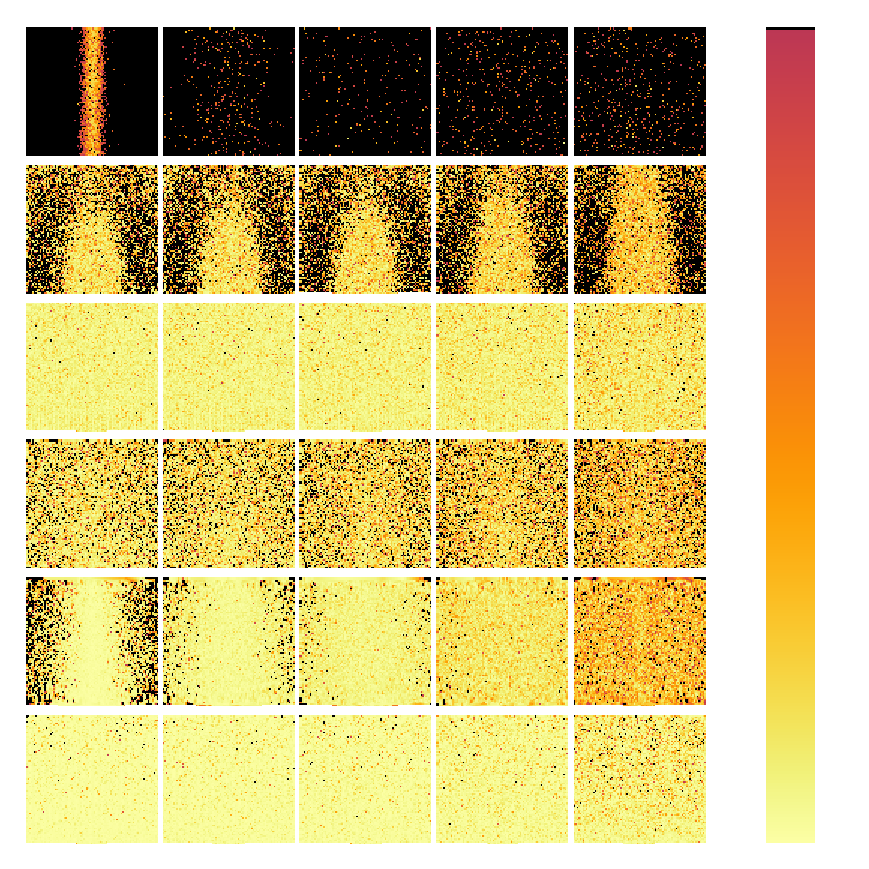
\includegraphics{./figures/parts/appendix/chapters/05/sections/04/caer_style_orientation_errors_dxyt4}}%
    \gplfronttext
  \end{picture}%
\endgroup

  \vspace{1cm}
  \caption{\small Χάρτες θερμότητας των μέτρων των τελικών σφαλμάτων εκτίμησης
           προσανατολισμού συναρτήσει των αρχικών σφαλμάτων εκτίμησης
           προσανατολισμού $\Delta\hat{\theta} \in
           [-\overline{\delta}_{\theta},+\overline{\delta}_{\theta}]$ (στον
           οριζόντιο άξονα) και των μέτρων των αρχικών σφαλμάτων εκτίμησης
           θέσης $\|\Delta \hat{\bm{l}}\|_2 \in [0, \sqrt{2}\cdot
           \overline{\delta}_{xy}]$ (στον κάθετο άξονα) για όλα τα
           διενεργηθέντα πειράματα, ανά αλγόριθμο και ανά τυπική απόκλιση
           διαταραχών του φυσικού αισθητήρα, για τη διάταξη με
           $(\overline{\delta}_{xy}, \overline{\delta}_{\theta}) = (0.20,
           0.30)$ [m,rad], εστιασμένοι στο διάστημα $[0,
           e_{xy,\text{avg}}^{\overline{\delta}_{xy},
           \overline{\delta}_{\theta}}]$, όπου με
           $e_{xy,\text{avg}}^{\overline{\delta}_{xy},
           \overline{\delta}_{\theta}}$ σημειώνεται ο μέσος όρος σφάλματος
           εκτίμησης στάσης όλων των μεθόδων, για κάθε επεξεργασθέν δείγμα, και
           κάθε τιμή τυπικής απόκλισης των διαταραχών που επιδρούν στις
           μετρήσεις του φυσικού αισθητήρα, για τη διαμόρφωση
           $(\overline{\delta}_{xy}, \overline{\delta}_{\theta})$.  Τιμές
           μέτρου σφάλματος εκτίμησης άνω του μέσου όρου σημειώνονται με μαύρο
           χρώμα}
  \label{fig:appendix_05_01:22}
\end{figure}
\begin{figure}\vspace{1cm}\hspace{0.5cm}
  % GNUPLOT: LaTeX picture with Postscript
\begingroup
  \makeatletter
  \providecommand\color[2][]{%
    \GenericError{(gnuplot) \space\space\space\@spaces}{%
      Package color not loaded in conjunction with
      terminal option `colourtext'%
    }{See the gnuplot documentation for explanation.%
    }{Either use 'blacktext' in gnuplot or load the package
      color.sty in LaTeX.}%
    \renewcommand\color[2][]{}%
  }%
  \providecommand\includegraphics[2][]{%
    \GenericError{(gnuplot) \space\space\space\@spaces}{%
      Package graphicx or graphics not loaded%
    }{See the gnuplot documentation for explanation.%
    }{The gnuplot epslatex terminal needs graphicx.sty or graphics.sty.}%
    \renewcommand\includegraphics[2][]{}%
  }%
  \providecommand\rotatebox[2]{#2}%
  \@ifundefined{ifGPcolor}{%
    \newif\ifGPcolor
    \GPcolorfalse
  }{}%
  \@ifundefined{ifGPblacktext}{%
    \newif\ifGPblacktext
    \GPblacktexttrue
  }{}%
  % define a \g@addto@macro without @ in the name:
  \let\gplgaddtomacro\g@addto@macro
  % define empty templates for all commands taking text:
  \gdef\gplfronttext{}%
  \gdef\gplfronttext{}%
  \makeatother
  \ifGPblacktext
    % no textcolor at all
    \def\colorrgb#1{}%
    \def\colorgray#1{}%
  \else
    % gray or color?
    \ifGPcolor
      \def\colorrgb#1{\color[rgb]{#1}}%
      \def\colorgray#1{\color[gray]{#1}}%
      \expandafter\def\csname LTw\endcsname{\color{white}}%
      \expandafter\def\csname LTb\endcsname{\color{black}}%
      \expandafter\def\csname LTa\endcsname{\color{black}}%
      \expandafter\def\csname LT0\endcsname{\color[rgb]{1,0,0}}%
      \expandafter\def\csname LT1\endcsname{\color[rgb]{0,1,0}}%
      \expandafter\def\csname LT2\endcsname{\color[rgb]{0,0,1}}%
      \expandafter\def\csname LT3\endcsname{\color[rgb]{1,0,1}}%
      \expandafter\def\csname LT4\endcsname{\color[rgb]{0,1,1}}%
      \expandafter\def\csname LT5\endcsname{\color[rgb]{1,1,0}}%
      \expandafter\def\csname LT6\endcsname{\color[rgb]{0,0,0}}%
      \expandafter\def\csname LT7\endcsname{\color[rgb]{1,0.3,0}}%
      \expandafter\def\csname LT8\endcsname{\color[rgb]{0.5,0.5,0.5}}%
    \else
      % gray
      \def\colorrgb#1{\color{black}}%
      \def\colorgray#1{\color[gray]{#1}}%
      \expandafter\def\csname LTw\endcsname{\color{white}}%
      \expandafter\def\csname LTb\endcsname{\color{black}}%
      \expandafter\def\csname LTa\endcsname{\color{black}}%
      \expandafter\def\csname LT0\endcsname{\color{black}}%
      \expandafter\def\csname LT1\endcsname{\color{black}}%
      \expandafter\def\csname LT2\endcsname{\color{black}}%
      \expandafter\def\csname LT3\endcsname{\color{black}}%
      \expandafter\def\csname LT4\endcsname{\color{black}}%
      \expandafter\def\csname LT5\endcsname{\color{black}}%
      \expandafter\def\csname LT6\endcsname{\color{black}}%
      \expandafter\def\csname LT7\endcsname{\color{black}}%
      \expandafter\def\csname LT8\endcsname{\color{black}}%
    \fi
  \fi
  \setlength{\unitlength}{0.0500bp}%
  \begin{picture}(8000.00,8000.00)%
     \gplgaddtomacro\gplfronttext{%
      \colorrgb{0.00,0.00,0.00}%
      \put(716,8200){\makebox(0,0){\strut{}\small $\sigma_R = 0.01$}}%
      \colorrgb{0.00,0.00,0.00}%
      \put(2029,8200){\makebox(0,0){\strut{}\small $\sigma_R = 0.03$}}%
      \colorrgb{0.00,0.00,0.00}%
      \put(3343,8200){\makebox(0,0){\strut{}\small $\sigma_R = 0.05$}}%
      \colorrgb{0.00,0.00,0.00}%
      \put(4656,8200){\makebox(0,0){\strut{}\small $\sigma_R = 0.10$}}%
      \colorrgb{0.00,0.00,0.00}%
      \put(5969,8200){\makebox(0,0){\strut{}\small $\sigma_R = 0.20$ [m]}}%
      \put(3333.33,8700){\makebox(0,0){\strut{}$(\overline{\delta}_{xy}, \overline{\delta}_\theta) = (0.20 \ \text{m}, 0.56 \ \text{rad})$}}
      \put(4000,9200){\makebox(0,0){\strut{}Τελικά σφάλματα εκτίμησης προσανατολισμού ως προς αρχικές συνθήκες μετατόπισης [rad]}}
    }%
    \gplgaddtomacro\gplfronttext{%
      \colorrgb{0.00,0.00,0.00}%
      \put(-200,7333.33){\rotatebox{90}{\makebox(0,0){\strut{}\small PLICP}}}%
    }%
    \gplgaddtomacro\gplfronttext{%
      \colorrgb{0.00,0.00,0.00}%
      \put(-200,6000){\rotatebox{90}{\makebox(0,0){\strut{}\small NDT}}}%
    }%
    \gplgaddtomacro\gplfronttext{%
      \colorrgb{0.00,0.00,0.00}%
      \put(-200,4666.66){\rotatebox{90}{\makebox(0,0){\strut{}\small FastGICP}}}%
    }%
    \gplgaddtomacro\gplfronttext{%
      \colorrgb{0.00,0.00,0.00}%
      \put(-200,3333.33){\rotatebox{90}{\makebox(0,0){\strut{}\small FastVGICP}}}%
    }%
    \gplgaddtomacro\gplfronttext{%
      \colorrgb{0.00,0.00,0.00}%
      \put(-200,2000){\rotatebox{90}{\makebox(0,0){\strut{}\small NDT-PSO}}}%
    }%
    \gplgaddtomacro\gplfronttext{%
      \colorrgb{0.00,0.00,0.00}%
      \put(-200,666.66){\rotatebox{90}{\makebox(0,0){\strut{}\small \texttt{fsm}}}}%
    }%
    \gplgaddtomacro\gplfronttext{%
      \colorrgb{0.00,0.00,0.00}%
      \put(7800,80){\makebox(0,0)[l]{\strut{}$0.0$}}%
      \colorrgb{0.00,0.00,0.00}%
      \put(7800,1111){\makebox(0,0)[l]{\strut{}$0.01$}}%
      \colorrgb{0.00,0.00,0.00}%
      \put(7800,2141){\makebox(0,0)[l]{\strut{}$0.02$}}%
      \colorrgb{0.00,0.00,0.00}%
      \put(7800,3172){\makebox(0,0)[l]{\strut{}$0.03$}}%
      \colorrgb{0.00,0.00,0.00}%
      \put(7800,4203){\makebox(0,0)[l]{\strut{}$0.04$}}%
      \colorrgb{0.00,0.00,0.00}%
      \put(7800,5234){\makebox(0,0)[l]{\strut{}$0.05$}}%
      \colorrgb{0.00,0.00,0.00}%
      \put(7800,6264){\makebox(0,0)[l]{\strut{}$0.06$}}%
      \colorrgb{0.00,0.00,0.00}%
      \put(7800,7295){\makebox(0,0)[l]{\strut{}$0.07$}}%
      \colorrgb{0.00,0.00,0.00}%
      \put(7800,7919){\makebox(0,0)[l]{\strut{}$> e^{\overline{\delta}_{xy}, \overline{\delta}_\theta}_{\theta,\text{avg}} = 0.0761$}}%
    }%
    \put(0,0){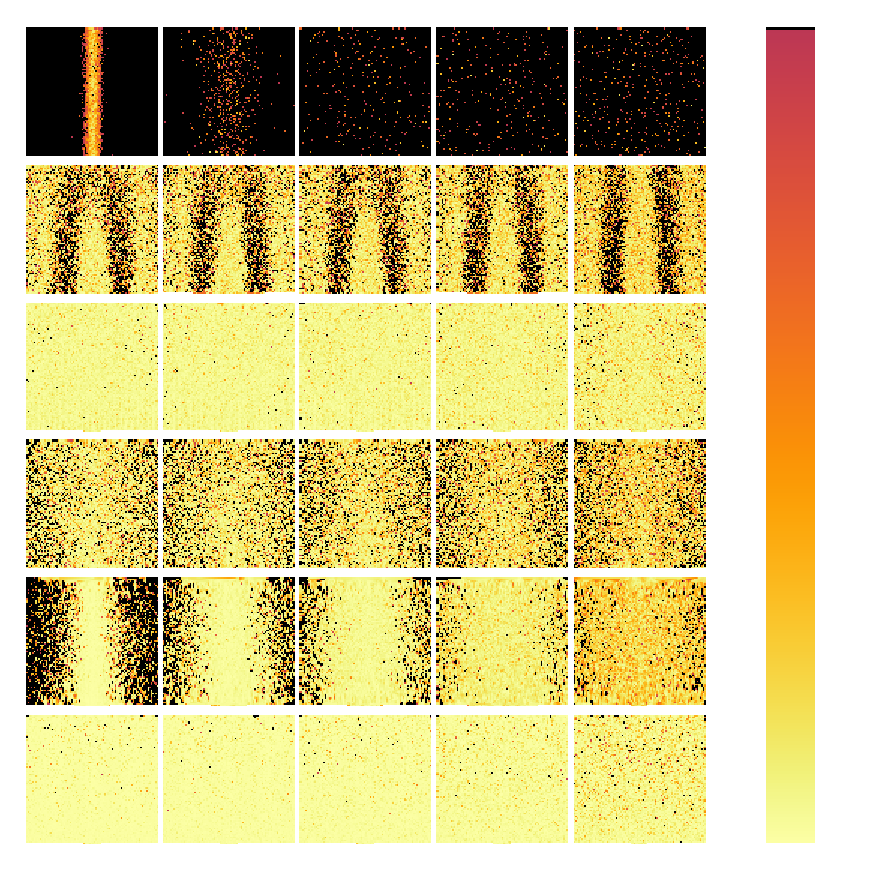
\includegraphics{./figures/parts/appendix/chapters/05/sections/04/caer_style_orientation_errors_dxyt5}}%
    \gplfronttext
  \end{picture}%
\endgroup

  \vspace{1cm}
  \caption{\small Χάρτες θερμότητας των μέτρων των τελικών σφαλμάτων εκτίμησης
           προσανατολισμού συναρτήσει των αρχικών σφαλμάτων εκτίμησης
           προσανατολισμού $\Delta\hat{\theta} \in
           [-\overline{\delta}_{\theta},+\overline{\delta}_{\theta}]$ (στον
           οριζόντιο άξονα) και των μέτρων των αρχικών σφαλμάτων εκτίμησης
           θέσης $\|\Delta \hat{\bm{l}}\|_2 \in [0, \sqrt{2}\cdot
           \overline{\delta}_{xy}]$ (στον κάθετο άξονα) για όλα τα
           διενεργηθέντα πειράματα, ανά αλγόριθμο και ανά τυπική απόκλιση
           διαταραχών του φυσικού αισθητήρα, για τη διάταξη με
           $(\overline{\delta}_{xy}, \overline{\delta}_{\theta}) = (0.20,
           0.56)$ [m,rad], εστιασμένοι στο διάστημα $[0,
           e_{xy,\text{avg}}^{\overline{\delta}_{xy},
           \overline{\delta}_{\theta}}]$, όπου με
           $e_{xy,\text{avg}}^{\overline{\delta}_{xy},
           \overline{\delta}_{\theta}}$ σημειώνεται ο μέσος όρος σφάλματος
           εκτίμησης στάσης όλων των μεθόδων, για κάθε επεξεργασθέν δείγμα, και
           κάθε τιμή τυπικής απόκλισης των διαταραχών που επιδρούν στις
           μετρήσεις του φυσικού αισθητήρα, για τη διαμόρφωση
           $(\overline{\delta}_{xy}, \overline{\delta}_{\theta})$.  Τιμές
           μέτρου σφάλματος εκτίμησης άνω του μέσου όρου σημειώνονται με μαύρο
           χρώμα}
  \label{fig:appendix_05_01:23}
\end{figure}
\begin{figure}\vspace{1cm}\hspace{0.5cm}
  % GNUPLOT: LaTeX picture with Postscript
\begingroup
  \makeatletter
  \providecommand\color[2][]{%
    \GenericError{(gnuplot) \space\space\space\@spaces}{%
      Package color not loaded in conjunction with
      terminal option `colourtext'%
    }{See the gnuplot documentation for explanation.%
    }{Either use 'blacktext' in gnuplot or load the package
      color.sty in LaTeX.}%
    \renewcommand\color[2][]{}%
  }%
  \providecommand\includegraphics[2][]{%
    \GenericError{(gnuplot) \space\space\space\@spaces}{%
      Package graphicx or graphics not loaded%
    }{See the gnuplot documentation for explanation.%
    }{The gnuplot epslatex terminal needs graphicx.sty or graphics.sty.}%
    \renewcommand\includegraphics[2][]{}%
  }%
  \providecommand\rotatebox[2]{#2}%
  \@ifundefined{ifGPcolor}{%
    \newif\ifGPcolor
    \GPcolorfalse
  }{}%
  \@ifundefined{ifGPblacktext}{%
    \newif\ifGPblacktext
    \GPblacktexttrue
  }{}%
  % define a \g@addto@macro without @ in the name:
  \let\gplgaddtomacro\g@addto@macro
  % define empty templates for all commands taking text:
  \gdef\gplfronttext{}%
  \gdef\gplfronttext{}%
  \makeatother
  \ifGPblacktext
    % no textcolor at all
    \def\colorrgb#1{}%
    \def\colorgray#1{}%
  \else
    % gray or color?
    \ifGPcolor
      \def\colorrgb#1{\color[rgb]{#1}}%
      \def\colorgray#1{\color[gray]{#1}}%
      \expandafter\def\csname LTw\endcsname{\color{white}}%
      \expandafter\def\csname LTb\endcsname{\color{black}}%
      \expandafter\def\csname LTa\endcsname{\color{black}}%
      \expandafter\def\csname LT0\endcsname{\color[rgb]{1,0,0}}%
      \expandafter\def\csname LT1\endcsname{\color[rgb]{0,1,0}}%
      \expandafter\def\csname LT2\endcsname{\color[rgb]{0,0,1}}%
      \expandafter\def\csname LT3\endcsname{\color[rgb]{1,0,1}}%
      \expandafter\def\csname LT4\endcsname{\color[rgb]{0,1,1}}%
      \expandafter\def\csname LT5\endcsname{\color[rgb]{1,1,0}}%
      \expandafter\def\csname LT6\endcsname{\color[rgb]{0,0,0}}%
      \expandafter\def\csname LT7\endcsname{\color[rgb]{1,0.3,0}}%
      \expandafter\def\csname LT8\endcsname{\color[rgb]{0.5,0.5,0.5}}%
    \else
      % gray
      \def\colorrgb#1{\color{black}}%
      \def\colorgray#1{\color[gray]{#1}}%
      \expandafter\def\csname LTw\endcsname{\color{white}}%
      \expandafter\def\csname LTb\endcsname{\color{black}}%
      \expandafter\def\csname LTa\endcsname{\color{black}}%
      \expandafter\def\csname LT0\endcsname{\color{black}}%
      \expandafter\def\csname LT1\endcsname{\color{black}}%
      \expandafter\def\csname LT2\endcsname{\color{black}}%
      \expandafter\def\csname LT3\endcsname{\color{black}}%
      \expandafter\def\csname LT4\endcsname{\color{black}}%
      \expandafter\def\csname LT5\endcsname{\color{black}}%
      \expandafter\def\csname LT6\endcsname{\color{black}}%
      \expandafter\def\csname LT7\endcsname{\color{black}}%
      \expandafter\def\csname LT8\endcsname{\color{black}}%
    \fi
  \fi
  \setlength{\unitlength}{0.0500bp}%
  \begin{picture}(8000.00,8000.00)%
     \gplgaddtomacro\gplfronttext{%
      \colorrgb{0.00,0.00,0.00}%
      \put(716,8200){\makebox(0,0){\strut{}\small $\sigma_R = 0.01$}}%
      \colorrgb{0.00,0.00,0.00}%
      \put(2029,8200){\makebox(0,0){\strut{}\small $\sigma_R = 0.03$}}%
      \colorrgb{0.00,0.00,0.00}%
      \put(3343,8200){\makebox(0,0){\strut{}\small $\sigma_R = 0.05$}}%
      \colorrgb{0.00,0.00,0.00}%
      \put(4656,8200){\makebox(0,0){\strut{}\small $\sigma_R = 0.10$}}%
      \colorrgb{0.00,0.00,0.00}%
      \put(5969,8200){\makebox(0,0){\strut{}\small $\sigma_R = 0.20$ [m]}}%
    }%
    \gplgaddtomacro\gplfronttext{%
      \colorrgb{0.00,0.00,0.00}%
      \put(-200,7333.33){\rotatebox{90}{\makebox(0,0){\strut{}\small PLICP}}}%
    }%
    \gplgaddtomacro\gplfronttext{%
      \colorrgb{0.00,0.00,0.00}%
      \put(-200,6000){\rotatebox{90}{\makebox(0,0){\strut{}\small NDT}}}%
    }%
    \gplgaddtomacro\gplfronttext{%
      \colorrgb{0.00,0.00,0.00}%
      \put(-200,4666.66){\rotatebox{90}{\makebox(0,0){\strut{}\small FastGICP}}}%
    }%
    \gplgaddtomacro\gplfronttext{%
      \colorrgb{0.00,0.00,0.00}%
      \put(-200,3333.33){\rotatebox{90}{\makebox(0,0){\strut{}\small FastVGICP}}}%
    }%
    \gplgaddtomacro\gplfronttext{%
      \colorrgb{0.00,0.00,0.00}%
      \put(-200,2000){\rotatebox{90}{\makebox(0,0){\strut{}\small NDT-PSO}}}%
    }%
    \gplgaddtomacro\gplfronttext{%
      \colorrgb{0.00,0.00,0.00}%
      \put(-200,666.66){\rotatebox{90}{\makebox(0,0){\strut{}\small \texttt{fsm}}}}%
    }%
    \gplgaddtomacro\gplfronttext{%
      \colorrgb{0.00,0.00,0.00}%
      \put(7800,80){\makebox(0,0)[l]{\strut{}$0.0$}}%
      \colorrgb{0.00,0.00,0.00}%
      \put(7800,1475){\makebox(0,0)[l]{\strut{}$0.02$}}%
      \colorrgb{0.00,0.00,0.00}%
      \put(7800,2871){\makebox(0,0)[l]{\strut{}$0.04$}}%
      \colorrgb{0.00,0.00,0.00}%
      \put(7800,4266){\makebox(0,0)[l]{\strut{}$0.06$}}%
      \colorrgb{0.00,0.00,0.00}%
      \put(7800,5661){\makebox(0,0)[l]{\strut{}$0.08$}}%
      \colorrgb{0.00,0.00,0.00}%
      \put(7800,7057){\makebox(0,0)[l]{\strut{}$0.10$}}%
      \colorrgb{0.00,0.00,0.00}%
      \put(7800,7919){\makebox(0,0)[l]{\strut{}$> 0.11236$}}%
    }%
    \put(0,0){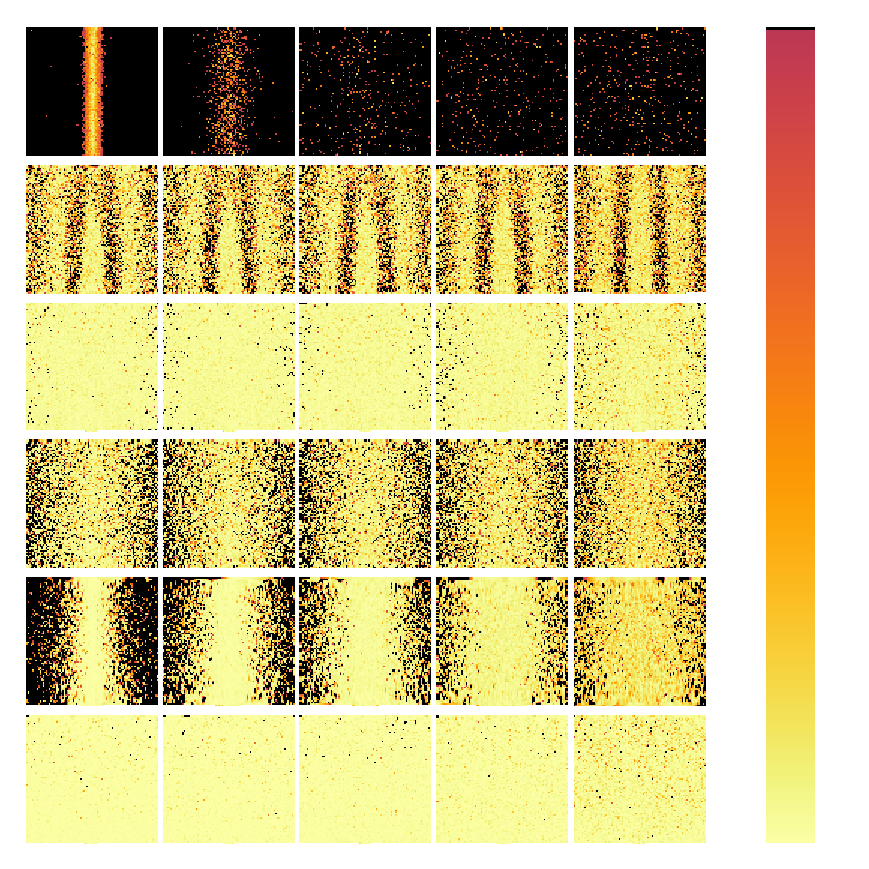
\includegraphics{./figures/parts/02/chapters/05/sections/04/caer_style_orientation_errors_dxyt6}}%
    \gplfronttext
  \end{picture}%
\endgroup

  \vspace{1cm}
  \caption{\small Χάρτες θερμότητας των μέτρων των τελικών σφαλμάτων εκτίμησης
           προσανατολισμού συναρτήσει των αρχικών σφαλμάτων εκτίμησης
           προσανατολισμού $\Delta\hat{\theta} \in
           [-\overline{\delta}_{\theta},+\overline{\delta}_{\theta}]$ (στον
           οριζόντιο άξονα) και των μέτρων των αρχικών σφαλμάτων εκτίμησης
           θέσης $\|\Delta \hat{\bm{l}}\|_2 \in [0, \sqrt{2}\cdot
           \overline{\delta}_{xy}]$ (στον κάθετο άξονα) για όλα τα
           διενεργηθέντα πειράματα, ανά αλγόριθμο και ανά τυπική απόκλιση
           διαταραχών του φυσικού αισθητήρα, για τη διάταξη με
           $(\overline{\delta}_{xy}, \overline{\delta}_{\theta}) = (0.20,
           \pi/4)$ [m,rad], εστιασμένοι στο διάστημα $[0,
           e_{xy,\text{avg}}^{\overline{\delta}_{xy},
           \overline{\delta}_{\theta}}]$, όπου με
           $e_{xy,\text{avg}}^{\overline{\delta}_{xy},
           \overline{\delta}_{\theta}}$ σημειώνεται ο μέσος όρος σφάλματος
           εκτίμησης στάσης όλων των μεθόδων, για κάθε επεξεργασθέν δείγμα, και
           κάθε τιμή τυπικής απόκλισης των διαταραχών που επιδρούν στις
           μετρήσεις του φυσικού αισθητήρα, για τη διαμόρφωση
           $(\overline{\delta}_{xy}, \overline{\delta}_{\theta})$.  Τιμές
           μέτρου σφάλματος εκτίμησης άνω του μέσου όρου σημειώνονται με μαύρο
           χρώμα}
  \label{fig:appendix_05_01:24}
\end{figure}
